% =====================================================================================
% Team 33 (P33) -- "Does Synthetic Data Help? GAN Augmentation for Small Medical Datasets"
% Report body, section by section. Meant to be pasted into the course's Computer Vision
% ELCVIA template; included by main.tex via % =====================================================================================
% Team 33 (P33) -- "Does Synthetic Data Help? GAN Augmentation for Small Medical Datasets"
% Report body, section by section. Meant to be pasted into the course's Computer Vision
% ELCVIA template; included by main.tex via % =====================================================================================
% Team 33 (P33) -- "Does Synthetic Data Help? GAN Augmentation for Small Medical Datasets"
% Report body, section by section. Meant to be pasted into the course's Computer Vision
% ELCVIA template; included by main.tex via % =====================================================================================
% Team 33 (P33) -- "Does Synthetic Data Help? GAN Augmentation for Small Medical Datasets"
% Report body, section by section. Meant to be pasted into the course's Computer Vision
% ELCVIA template; included by main.tex via \input{report_content}.
% Every number comes from results/ in the repository (see the table/figure captions).
% =====================================================================================

\begin{abstract}
Medical image datasets are often small and class-imbalanced, which limits how well deep classifiers can be trained.
We study whether images generated by a Generative Adversarial Network (GAN) can make up for this.
We train a class-conditional DCGAN on the training split of BreastMNIST (546 breast ultrasound images, 27\% malignant)
and add 0, 50, 100 or 200\% synthetic images to the training set of a CNN classifier, which is always evaluated on the
same held-out set of \emph{real} test images. To separate the effect of the \emph{amount} of synthetic data from its
\emph{quality}, we repeat every experiment with an early generator checkpoint (FID 134.9) and the fully trained
generator (FID 86.4; the real-vs-real reference is 59.1), compare against classical flip/shift augmentation and
against GAN-based class balancing, run five random seeds per setting, and test significance with Welch's $t$-test.
The generator learns realistic images without memorising the training set, and the better generator consistently beats
the worse one. Yet no amount of synthetic data improves macro F1 over real-only training (0.812; changes from $-0.054$ to
$+0.006$, none significant), while simple flip/shift augmentation gives the best F1 (0.834). Adding 200\% synthetic images
yields the highest AUC (0.922 vs.\ 0.911) but lowers malignant recall.
A second, nine times larger dataset (PneumoniaMNIST) is used to check whether the conclusion depends on dataset size.
All code, results and an interactive demo are available at \url{https://github.com/Bhagwati23/GAN-medicalAugmentation}.

\vspace{0.5cm}
\noindent
{\em Key Words}: Generative Adversarial Networks, DCGAN, Data Augmentation, Medical Image Classification,
Synthetic Data, MedMNIST, FID.
\end{abstract}
\hrulefill

% -------------------------------------------------------------------------------------
\section{Introduction}
Deep convolutional networks need many labelled examples, but labelled medical images are expensive: they require
expert annotation, are protected by privacy rules, and positive (disease) cases are rare. The usual remedy is
\emph{data augmentation}: creating new training examples from existing ones. Classical augmentation applies simple
geometric or photometric transforms (flips, shifts, rotations, contrast changes)~\cite{shorten2019survey}. Generative
Adversarial Networks (GANs)~\cite{goodfellow2014gan} offer a more ambitious option: learn the distribution of the
training images and sample entirely new ones. Frid-Adar et al.~\cite{fridadar2018gan} reported that GAN-generated
liver-lesion images raised CNN sensitivity and specificity, which made GAN augmentation popular in medical
imaging~\cite{yi2019ganmedical}.

However, a GAN trained on a small dataset only sees the same few hundred images as the classifier. It is therefore not
obvious that its samples add \emph{new information}; they may only add noise, or copies of the training images.
This project asks a precise question:

\begin{quote}
\emph{When a classifier is trained on a small medical dataset, does adding GAN-generated images improve its performance
on real, unseen images -- and how does the gain depend on the amount and on the quality of the synthetic data?}
\end{quote}

\noindent\textbf{Contributions.}
\begin{itemize}
  \item A reproducible pipeline (MedMNIST v2 data, class-conditional DCGAN, augmentation at 0/\allowbreak 50/\allowbreak 100/\allowbreak 200\%, CNN
        classifier, FID/KID evaluation) with strict separation of training, validation and test data.
  \item A two-axis study: \emph{quantity} (four synthetic ratios) $\times$ \emph{quality} (early vs.\ final generator,
        measured by FID and KID), plus two reference points: classical flip/shift augmentation and GAN class balancing.
  \item Statistical care: five seeds per setting, mean $\pm$ standard deviation, Welch's $t$-test against the real-only baseline.
  \item Checks that the generator does not simply memorise the training set (nearest-neighbour distances and latent
        interpolation).
  \item A replication on a second, larger dataset (PneumoniaMNIST) and an interactive web demo.
\end{itemize}

\begin{keybox}{Key findings at a glance}
\begin{itemize}
  \item \textbf{No F1 gain from GAN images} on either dataset at 50, 100 or 200\% synthetic data (BreastMNIST real-only
        F1 0.812 vs.\ 0.758--0.819 with GAN data; none significant, all $p>0.2$).
  \item \textbf{Quality matters:} the better generator (FID 86) beats the early one (FID 135) in AUC at every ratio.
  \item \textbf{200\% synthetic gives the best AUC} on both datasets (0.922 and 0.976) and, on the larger dataset,
        cuts seed-to-seed variance five-fold.
  \item \textbf{No memorisation:} no generated image is closer to a training image than typical unseen real images.
  \item \textbf{Classical augmentation depends on anatomy:} best for breast ultrasound (F1 0.834), harmful for chest
        X-rays (F1 0.755) because mirrored chests are anatomically wrong.
\end{itemize}
\end{keybox}

% -------------------------------------------------------------------------------------
\section{Related Work}
\textbf{GANs and DCGAN.} A GAN~\cite{goodfellow2014gan} trains a generator $G$ to map random noise $z$ to images and a
discriminator $D$ to tell real from generated images; the two are trained against each other. DCGAN~\cite{radford2016dcgan}
gave architectural rules that make this training stable for images: strided (transposed) convolutions instead of pooling,
batch normalisation, ReLU in $G$, LeakyReLU in $D$, Adam with learning rate $2\times10^{-4}$ and $\beta_1=0.5$.
Conditional GANs~\cite{mirza2014cgan} feed the class label to both networks so that images of a chosen class can be requested.

\textbf{GANs with little data.} With few training images the discriminator quickly memorises them and stops giving
useful gradients. DiffAugment~\cite{zhao2020diffaugment} applies the same random, differentiable augmentation to real and
generated images before the discriminator, which strongly improves GANs trained on a few hundred images.

\textbf{GAN augmentation in medical imaging.} Frid-Adar et al.~\cite{fridadar2018gan} generated liver-lesion CT patches
with DCGAN and improved classification from 78.6\% to 85.7\% sensitivity. Reviews~\cite{yi2019ganmedical} report
mixed results in later work, often without multiple seeds or a comparison with classical augmentation -- gaps this
project addresses.

\textbf{Evaluating generated images.} The Fr\'echet Inception Distance (FID)~\cite{heusel2017fid} compares Inception-v3
feature statistics of real and generated images; the Kernel Inception Distance (KID)~\cite{binkowski2018kid} is an
unbiased alternative better suited to small samples. Ravuri and Vinyals~\cite{ravuri2019cas} showed that such scores do not
fully predict how useful samples are for training a classifier -- which is exactly what our classifier experiments measure.

\textbf{MedMNIST.} MedMNIST v2~\cite{yang2023medmnist} provides standardised, pre-split 28$\times$28 biomedical datasets with
benchmark results, which makes our numbers comparable and reproducible.

% -------------------------------------------------------------------------------------
\section{Datasets}
We use two binary datasets from MedMNIST v2~\cite{yang2023medmnist} at their default 28$\times$28 grayscale resolution and
keep the \emph{official} train/validation/test splits (Table~\ref{tab:data}, Fig.~\ref{fig:data}).

\textbf{BreastMNIST} (main dataset) is derived from a breast ultrasound dataset~\cite{aldhabyani2020busi}; the label is
\emph{malignant} (class 0) or \emph{normal/benign} (class 1). With only 546 training images and 27\% malignant cases it is
exactly the small, imbalanced setting in which synthetic data is supposed to help.

\textbf{PneumoniaMNIST} (second dataset) is derived from paediatric chest X-rays~\cite{kermany2018pneumonia}: \emph{normal}
(class 0) vs.\ \emph{pneumonia} (class 1), with 4{,}708 training images (about nine times more). It tells us whether a
conclusion drawn on BreastMNIST changes when real data is more plentiful.

\begin{table}[htbp]
\centering
\caption{Official MedMNIST v2 splits (images per class). Source: \texttt{results/dataset\_stats.json}.}
\label{tab:data}
\begin{tabular}{llrrr}
\toprule
Dataset & Class & Train & Val & Test \\
\midrule
BreastMNIST    & malignant      & 147   & 21  & 42  \\
               & normal/benign  & 399   & 57  & 114 \\
               & \emph{total}   & 546   & 78  & 156 \\
\midrule
PneumoniaMNIST & normal         & 1{,}214 & 135 & 234 \\
               & pneumonia      & 3{,}494 & 389 & 390 \\
               & \emph{total}   & 4{,}708 & 524 & 624 \\
\bottomrule
\end{tabular}
\end{table}

\begin{figure}[htbp]
\centering
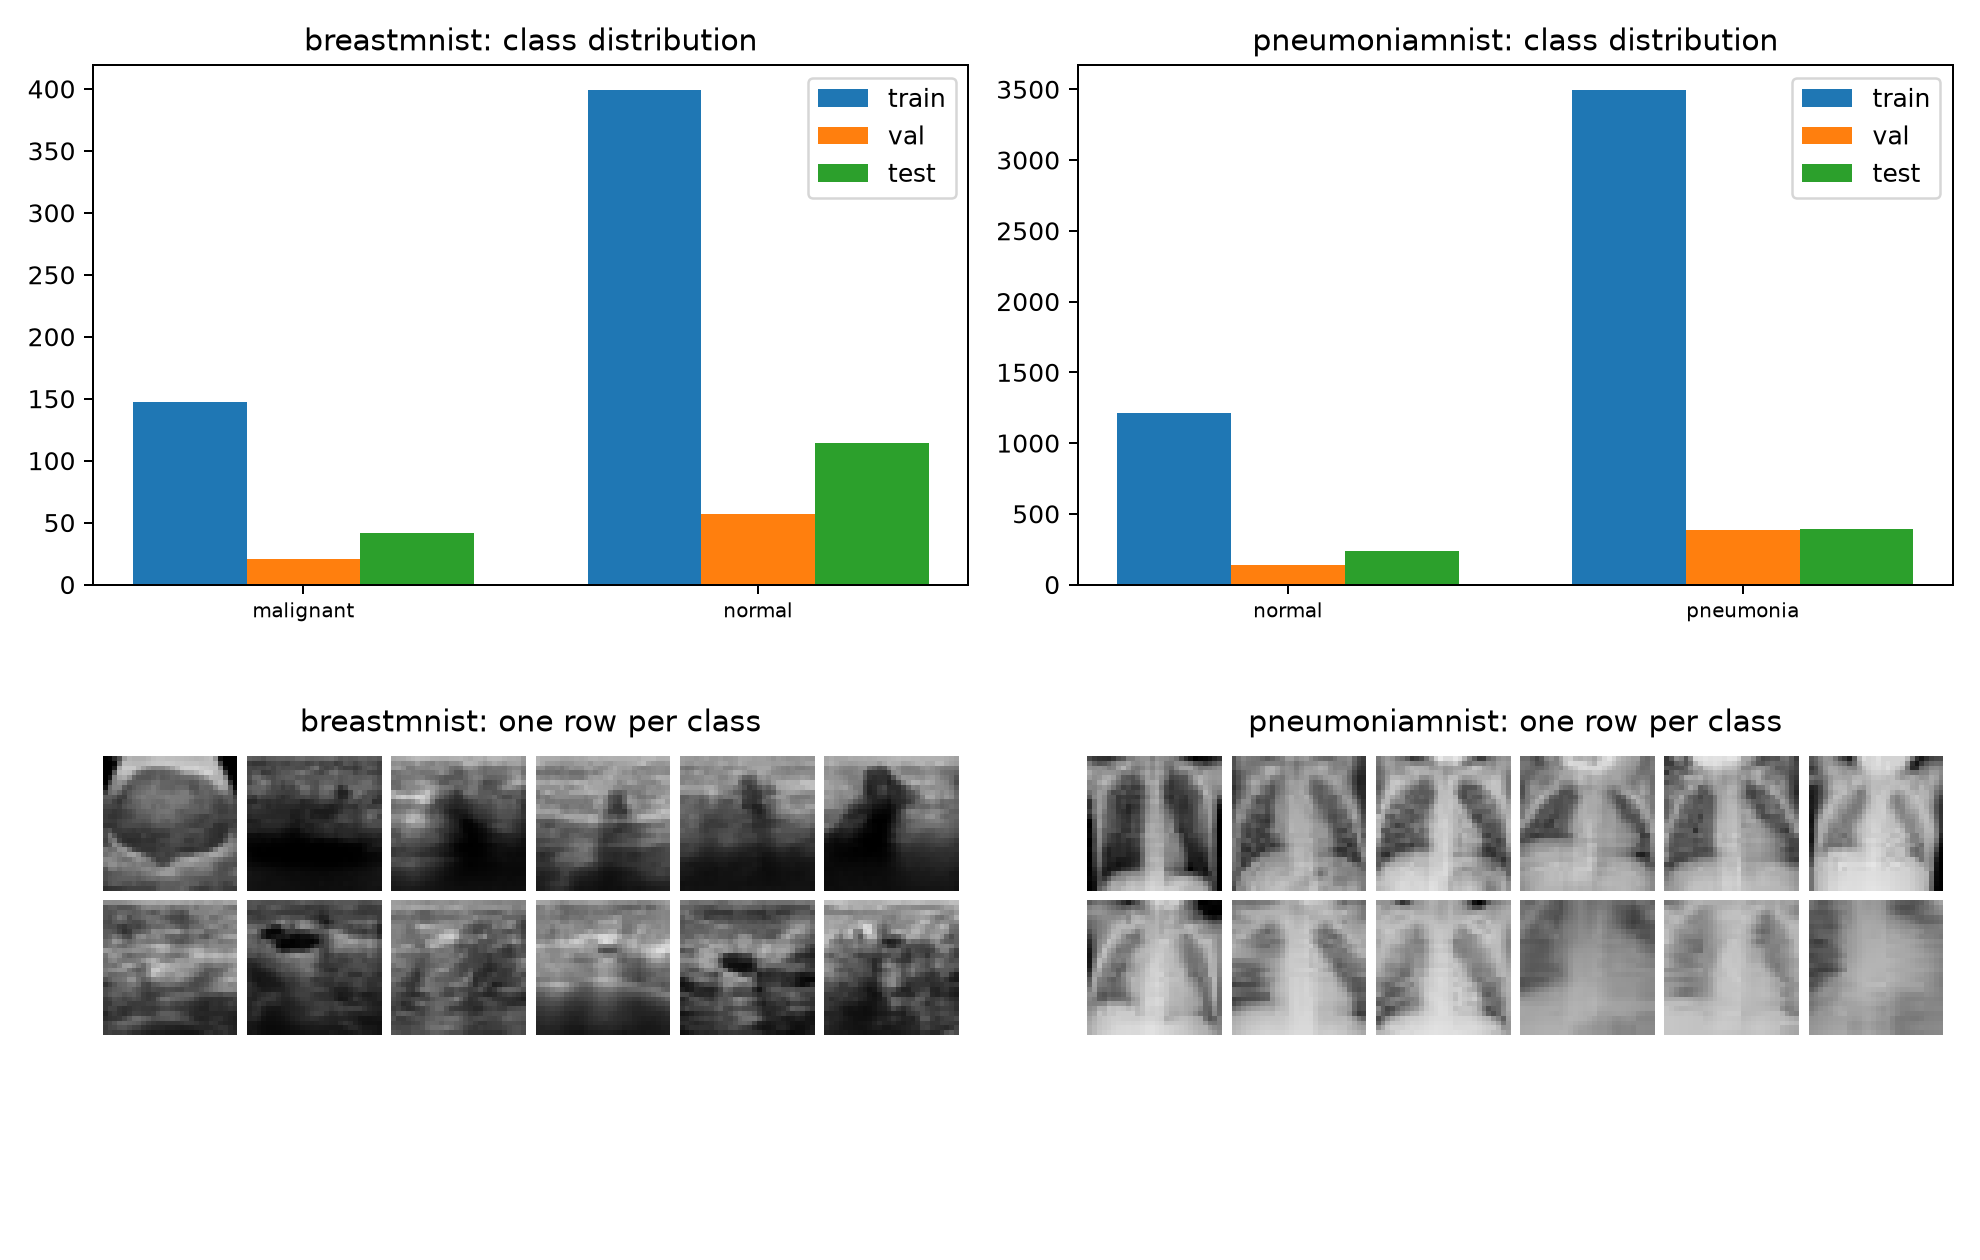
\includegraphics[width=\linewidth]{figures/dataset_overview.png}
\caption{Class distribution per split (top) and training images, one row per class (bottom). Both datasets are imbalanced
(minority class: malignant in BreastMNIST, normal in PneumoniaMNIST).}
\label{fig:data}
\end{figure}

\textbf{Preprocessing and leakage control.} Pixel values are scaled from $[0,255]$ to $[-1,1]$, the output range of the
generator's $\tanh$. The GAN is trained \emph{only} on the training split. Synthetic images are added \emph{only} to the
training split. Validation (used to choose the best epoch) and test (used once, for the final numbers) contain only real
images and are identical in every experiment. These rules are enforced in code and checked by unit tests.

% -------------------------------------------------------------------------------------
\section{Method}

\subsection{Pipeline}
\begin{enumerate}
  \item Train a class-conditional DCGAN on the real training images; save an \emph{early} checkpoint (after 10\% of
        training) and the \emph{final} one.
  \item Score both generators with FID and KID against the real training images, and check for memorisation.
  \item For each setting (Section~\ref{sec:settings}), build a training set of real images plus a controlled number of
        synthetic images, train the CNN classifier with five seeds, and evaluate on the real test set.
  \item Compare every setting with the real-only baseline (mean, standard deviation, Welch's $t$-test).
\end{enumerate}

\subsection{Class-conditional DCGAN}
Table~\ref{tab:gan} lists the architecture. The generator concatenates a 100-dimensional Gaussian noise vector $z$ with a
learned 50-dimensional embedding of the class label $y$, projects it to a $256\times7\times7$ tensor and upsamples it with
two stride-2 transposed convolutions to $28\times28$. The discriminator receives the image together with a learned
$28\times28$ ``label map'' as a second channel, so it judges whether the image is realistic \emph{for that class}.
Following DCGAN~\cite{radford2016dcgan}, weights are initialised from $\mathcal{N}(0,0.02)$, $G$ uses BatchNorm + ReLU and
$D$ uses LeakyReLU(0.2), no pooling layers.

\begin{table}[htbp]
\centering
\caption{Conditional DCGAN architecture (\texttt{ganaug/dcgan.py}). ConvT = transposed convolution, k = kernel, s = stride.}
\label{tab:gan}
\small
\begin{tabular}{ll}
\toprule
\multicolumn{2}{l}{\textbf{Generator} (2.56\,M parameters)} \\
Input & $z\in\mathbb{R}^{100}$ $\oplus$ Embedding$(y)\in\mathbb{R}^{50}$ \\
Linear + BN + ReLU & $150 \rightarrow 256\times7\times7$ \\
ConvT k4 s2 + BN + ReLU & $\rightarrow 128\times14\times14$ \\
ConvT k4 s2 + BN + ReLU & $\rightarrow 64\times28\times28$ \\
Conv k3 s1 + $\tanh$ & $\rightarrow 1\times28\times28$, values in $[-1,1]$ \\
\midrule
\multicolumn{2}{l}{\textbf{Discriminator} (0.43\,M parameters)} \\
Input & image $\oplus$ label map $\rightarrow 2\times28\times28$ \\
Conv k4 s2 + LeakyReLU & $\rightarrow 64\times14\times14$ \\
Conv k4 s2 + BN + LeakyReLU & $\rightarrow 128\times7\times7$ \\
Conv k3 s2 + BN + LeakyReLU & $\rightarrow 256\times4\times4$ \\
Dropout(0.3) + Linear & $\rightarrow$ 1 logit (real/fake) \\
\bottomrule
\end{tabular}
\end{table}

\textbf{Training objective.} With $\sigma$ the sigmoid and $\tilde{x}=T(x)$ a random translation (below), $D$ minimises
\begin{equation}
\mathcal{L}_D = -\,\mathbb{E}_{x,y}\big[\,0.9\log\sigma(D(\tilde{x},y))\big] - \mathbb{E}_{z,y}\big[\log\big(1-\sigma(D(\widetilde{G(z,y)},y))\big)\big],
\end{equation}
and $G$ minimises the non-saturating loss $\mathcal{L}_G = -\,\mathbb{E}_{z,y}\big[\log\sigma(D(\widetilde{G(z,y)},y))\big]$.
Two additions help with only 546 training images:
(i) \emph{one-sided label smoothing}: the target for real images is 0.9 instead of 1, so $D$ does not become over-confident;
(ii) \emph{DiffAugment-style translation}~\cite{zhao2020diffaugment}: every real and generated image is shifted by a random
$-2\ldots2$ pixels (edge-replicate padding) before it is shown to $D$, which keeps $D$ from memorising the training images.
Both networks use Adam ($2\times10^{-4}$, $\beta=(0.5,0.999)$), batch size 64.

\subsection{Augmentation protocol}
\label{sec:aug}
For a ratio $r\in\{0, 0.5, 1, 2\}$ we add $\mathrm{round}(r\cdot n_c)$ synthetic images of each class $c$, where $n_c$ is
the number of real training images of class $c$. This keeps the real class ratio (for BreastMNIST: $+50\%$ = 274,
$+100\%$ = 546, $+200\%$ = 1{,}092 synthetic images). For each generator we sample one fixed pool of synthetic images
(fixed seed) and every ratio takes the first $k$ images of each class, so the sets are \emph{nested}
($50\% \subset 100\% \subset 200\%$): differences between ratios come from the amount of data, not from a luckier draw.
In the \emph{class-balancing} setting we instead add only minority-class images until both classes have the same size
(BreastMNIST: 252 synthetic malignant images, giving 399 vs.\ 399).

\subsection{Classifier}
All settings use the same CNN (\texttt{ganaug/cnn.py}, 0.29\,M parameters): three blocks of
[Conv3$\times$3--BN--ReLU]$\times$2 + MaxPool with 32, 64 and 128 channels ($28\to14\to7\to3$), global average pooling,
dropout 0.3 and a linear layer. It is trained with cross-entropy, AdamW (learning rate $10^{-3}$, weight decay $10^{-4}$),
a cosine learning-rate schedule and batch size 64. After each epoch we compute the validation ROC-AUC and keep the weights
with the best value (model selection on validation, never on test). The model is deliberately small: the dataset is tiny
and all experiments ran on a CPU. Our real-only baseline (Section~\ref{sec:results}) is in line with the ResNet-18 results
reported by MedMNIST v2~\cite{yang2023medmnist} (BreastMNIST, 28$\times$28: accuracy 0.863, AUC 0.901).

\subsection{Evaluation}
\textbf{Classifier metrics} (real test set): accuracy; \emph{macro} precision, recall and F1 (each class weighted
equally, so missing the minority class is penalised; macro recall equals balanced accuracy); ROC-AUC (threshold-free
ranking quality); and confusion matrices. Macro F1 is our main metric because accuracy can look good on imbalanced data
by mostly predicting the majority class.

\textbf{Image quality.} FID and KID are computed with \texttt{torch-fidelity} between the real training images and the
same number of generated images with the same class ratio (images converted to 3-channel uint8 and resized to
299$\times$299 for Inception-v3). Because 28$\times$28 grayscale ultrasound images are very different from ImageNet photos,
absolute FID values are not comparable to natural-image papers; we therefore also report FID between the real training and
real test images as a \emph{reference floor}.

\textbf{Memorisation check.} For every generated image we find the closest real training image (pixel $L_2$ distance) and
compare these distances with the same distances for real \emph{test} images, which are realistic but unseen. A generator
that copies training images would produce many samples closer to the training set than almost any real test image; we
report the fraction of generated images closer than the 5th percentile of the test distances (about 0.05 is expected if
there is no copying).

\textbf{Statistics.} Each setting is trained with seeds 0--4 (BreastMNIST) or 0--2 (PneumoniaMNIST); we report mean
$\pm$ standard deviation and a two-sided Welch's $t$-test of the per-seed macro F1 against the real-only baseline.

% -------------------------------------------------------------------------------------
\section{Experimental Setup}
\label{sec:settings}
\begin{table}[htbp]
\centering
\caption{Experiment settings. Only the training set changes; the CNN, its hyper-parameters, and the validation and test
sets are identical everywhere.}
\label{tab:settings}
\small
\begin{tabular}{lp{5.2cm}}
\toprule
Setting & Training data \\
\midrule
Real only (0\%) & real training images (baseline) \\
Real + flip/shift & real images, random horizontal flip and $\pm2$\,px shift on the fly \\
+50/100/200\% GAN (final) & real + synthetic from the final generator \\
+50/100/200\% GAN (early) & real + synthetic from the early generator \\
GAN class balancing & real + synthetic minority-class images until classes are equal \\
\bottomrule
\end{tabular}
\end{table}

\begin{table}[htbp]
\centering
\caption{Training configuration.}
\label{tab:hparams}
\small
\begin{tabular}{lll}
\toprule
 & BreastMNIST & PneumoniaMNIST \\
\midrule
GAN epochs (updates)       & 300 (2{,}400) & 60 (4{,}380) \\
Early checkpoint           & epoch 30      & epoch 6 \\
Classifier epochs          & 40            & 15 \\
Seeds per setting          & 5             & 3 \\
Settings run               & all 9         & 7 (no early 50/200\%) \\
FID sample size            & 546           & 2{,}000 (random subset) \\
\bottomrule
\end{tabular}
\end{table}

All experiments ran on a laptop CPU with PyTorch. Table~\ref{tab:settings} lists the settings and Table~\ref{tab:hparams}
the configuration. Because PneumoniaMNIST is nine times larger, we used fewer classifier epochs, seeds and settings for it.
Everything is reproduced by \texttt{bash run\_all.sh}.

% -------------------------------------------------------------------------------------
\FloatBarrier
\section{Results}
\label{sec:results}

\subsection{Quality of the synthetic images}
\textbf{Training dynamics.} Figure~\ref{fig:losses} shows that GAN training on BreastMNIST stayed balanced for all 300
epochs: the discriminator loss stays close to $2\ln 2\approx1.39$ (the value when $D$ cannot separate real from fake), and
at the end $D$ assigns on average 0.46 to real and 0.44 to generated images. There is no sign of mode collapse (where
$D(G(z))$ would drop to 0 and all samples would look alike) or of $D$ winning outright.

\textbf{Reproducibility of GAN training.} The GAN training was run twice, independently, on two different laptops with
the same code, configuration and seed: run~1 produced the generators used for every experiment in this report, and run~2
(by Bhagwati, committed as the training log in \texttt{results/}) checks that training can be repeated. Averaged over the
last 10\% of epochs, the two runs agree closely: BreastMNIST discriminator loss 1.371 vs.\ 1.377, $D(x)$ 0.459 vs.\ 0.456
and $D(G(z))$ 0.441 vs.\ 0.444; PneumoniaMNIST discriminator loss 1.376 vs.\ 1.377, $D(x)$ 0.455 vs.\ 0.456. Bit-exact
equality is not expected, because CPU floating-point operations are not deterministic across machines and library
versions, but the training reaches the same balanced state.

\begin{figure}[htbp]
\centering
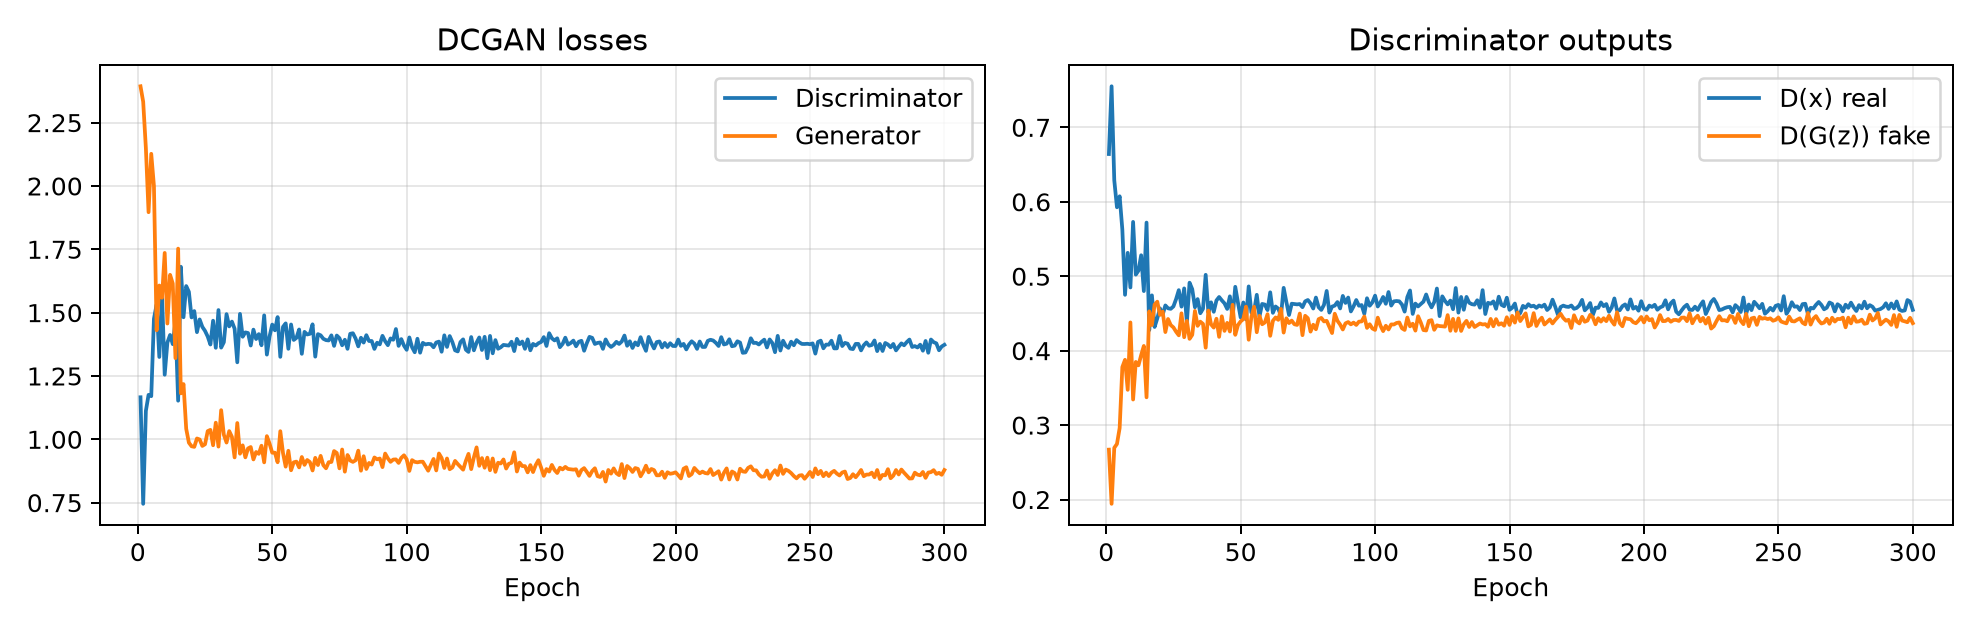
\includegraphics[width=\linewidth]{figures/breast_gan_losses.png}
\caption{DCGAN training on BreastMNIST. Left: losses. Right: mean discriminator output for real ($D(x)$) and generated
($D(G(z))$) images; both stay close to 0.5, i.e.\ a balanced adversarial game. Source: \texttt{results/breastmnist/report\_run/gan\_losses.csv} (run~1).}
\label{fig:losses}
\end{figure}

\textbf{Visual quality.} Figure~\ref{fig:samples} compares real images with samples from both generators. After 30 epochs
the generator only reproduces the global layout (bright tissue at the top, dark region at the bottom) with heavy noise.
After 300 epochs the samples contain lesion-like dark regions and ultrasound speckle texture; synthetic \emph{malignant}
images tend to show larger, darker, irregular masses, matching the real malignant row. Small checkerboard artefacts from
the transposed convolutions remain.

\begin{figure}[htbp]
\centering
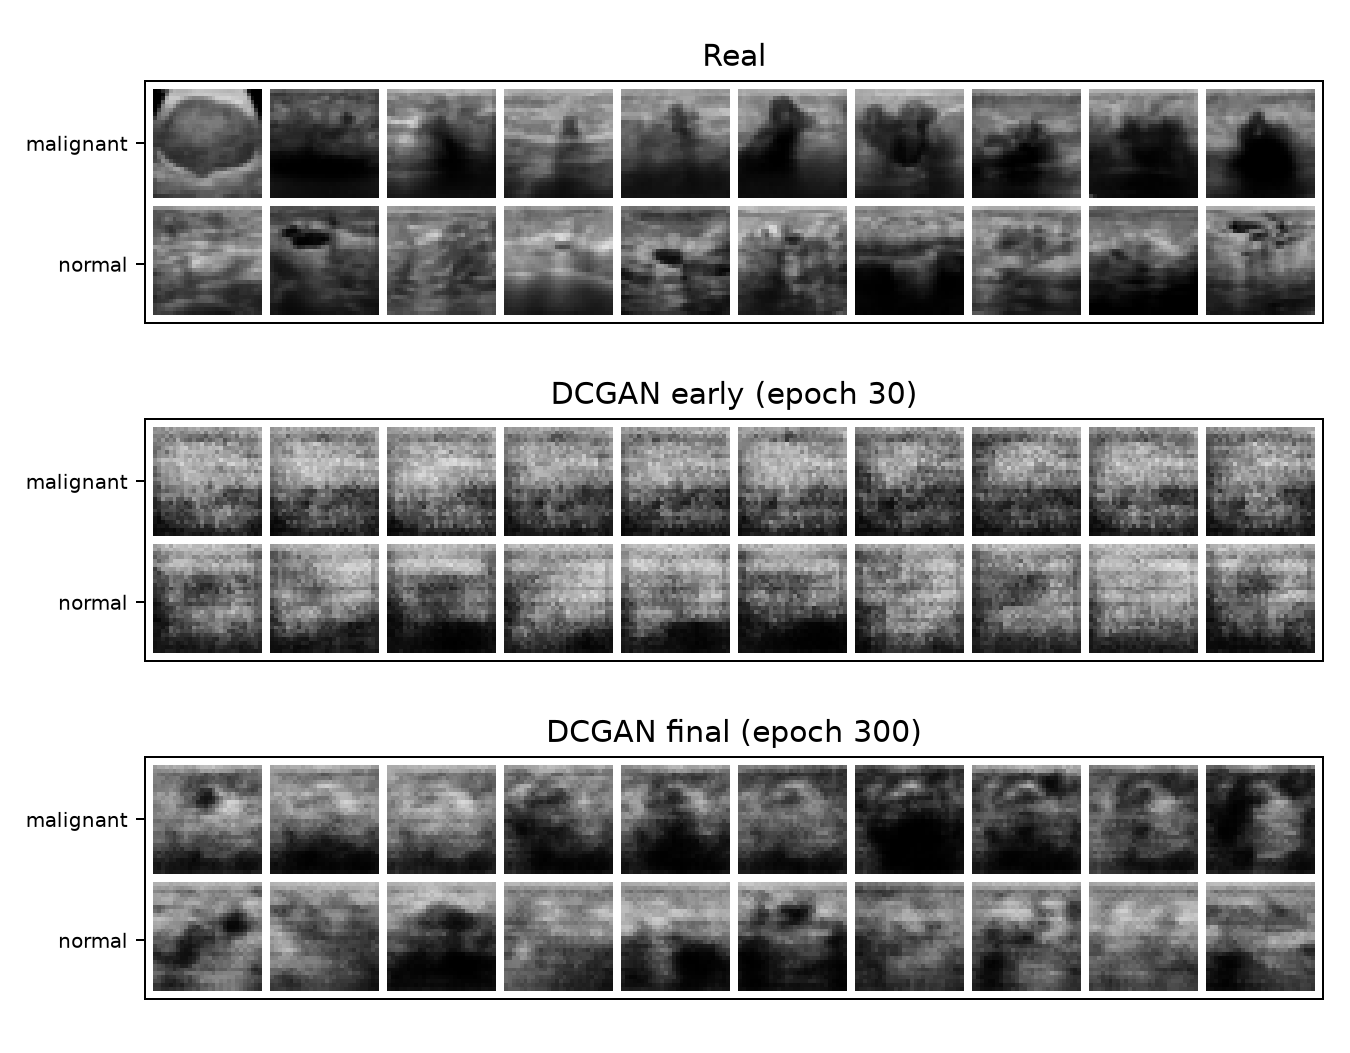
\includegraphics[width=0.9\linewidth]{figures/breast_real_vs_synthetic.png}
\caption{BreastMNIST: real training images (top), early generator after 30 epochs (middle) and final generator after 300
epochs (bottom); one row per class.}
\label{fig:samples}
\end{figure}

\textbf{FID and KID.} Table~\ref{tab:fid} quantifies the quality difference. The final generator reduces FID from 134.9 to
86.4 and KID by about half, but a gap to the real-vs-real reference (59.1) remains: the synthetic distribution is
clearly closer to the real one, yet not identical.

\begin{table}[htbp]
\centering
\caption{Image quality on BreastMNIST (546 images per set; lower is better). Source: \texttt{results/breastmnist/fid.json}.}
\label{tab:fid}
\small
\begin{tabular}{lrr}
\toprule
Compared with real training images & FID & KID \\
\midrule
Real test images (reference floor)   & 59.1  & 0.0004 \\
Early generator (epoch 30)           & 134.9 & 0.1220 \\
Final generator (epoch 300)          & 86.4  & 0.0670 \\
\bottomrule
\end{tabular}
\end{table}

\textbf{No memorisation.} The median distance from a generated image to its nearest training image is 6.33 (final) and
6.96 (early), larger than the 5.52 measured for real test images, and \emph{none} of the generated images is closer to a
training image than the closest 5\% of real test images (fraction 0.00 for both generators). Figure~\ref{fig:nn} shows
generated images next to their nearest training images: they share style but are not copies. The same figure also
shows a weakness: the first two generated images are almost identical to each other, a sign of \emph{limited diversity}
(partial mode collapse) -- the generator does not copy training images, but it also covers fewer distinct variations
than the real data. The latent interpolation in
Figure~\ref{fig:interp} changes smoothly from one image to another, which indicates that the generator learned a continuous
image distribution rather than a lookup table of training images.

\begin{figure}[htbp]
\centering
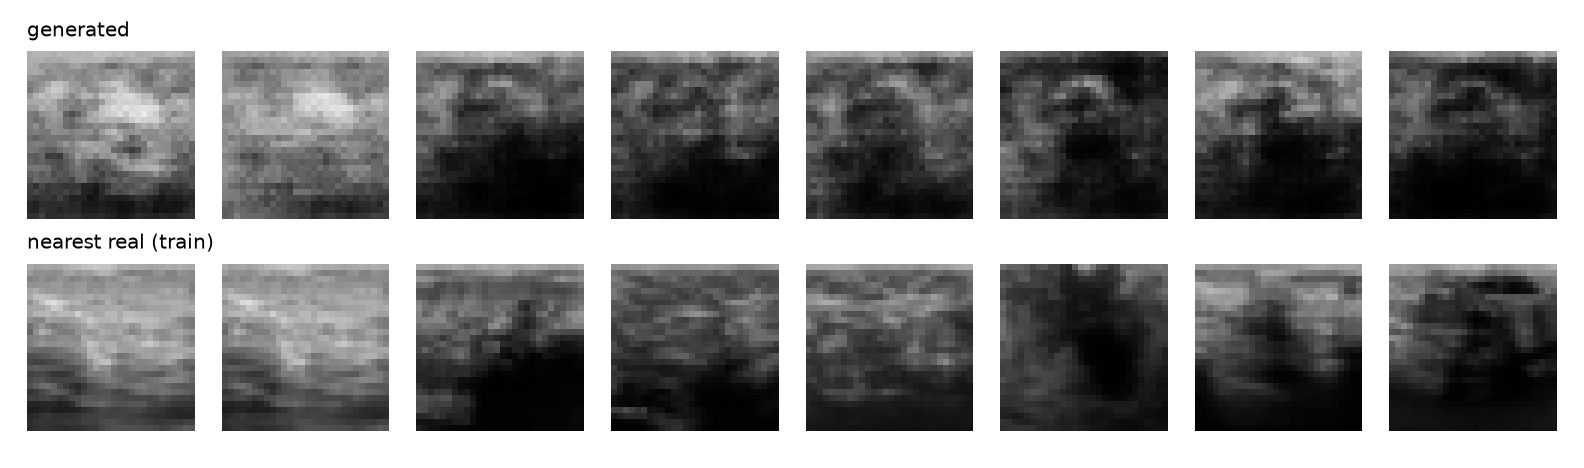
\includegraphics[width=\linewidth]{figures/breast_nearest_neighbours.png}
\caption{Top: images from the final generator. Bottom: the closest real training image to each (pixel $L_2$). Similar
style, different content: the generator does not copy training images. The first two samples are near-duplicates of
each other, showing limited sample diversity.}
\label{fig:nn}
\end{figure}

\begin{figure}[htbp]
\centering
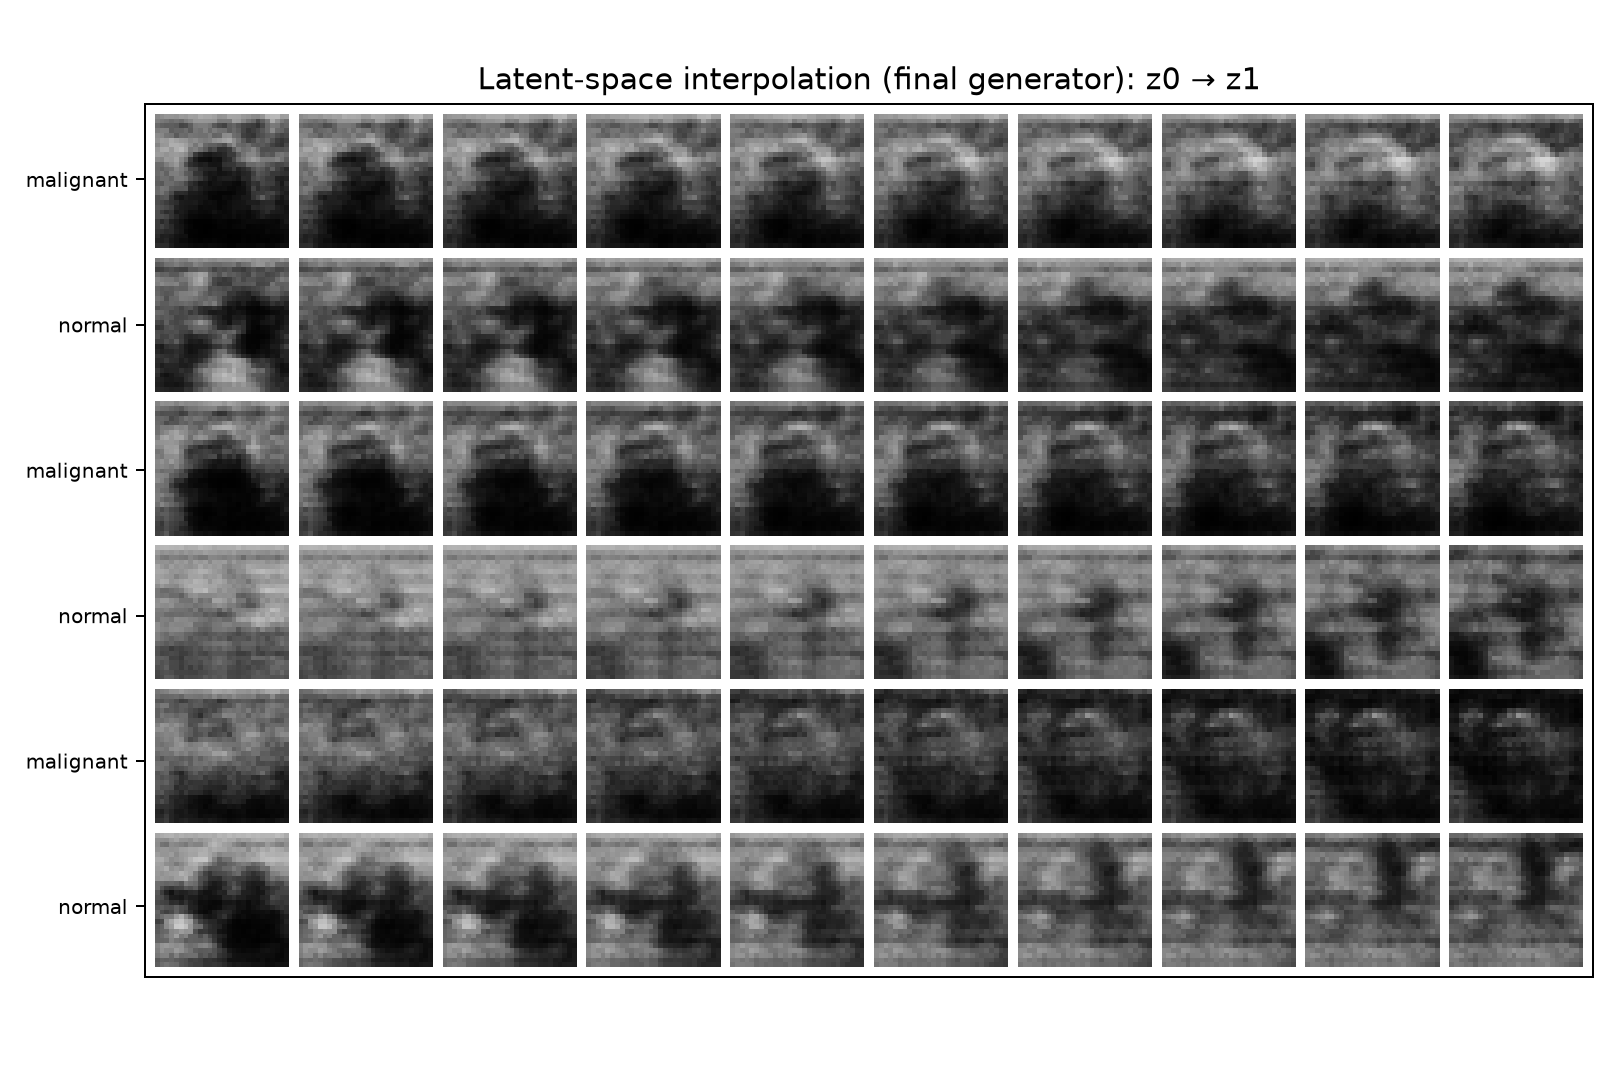
\includegraphics[width=0.85\linewidth]{figures/breast_interpolation.png}
\caption{Linear interpolation between two noise vectors $z_0\to z_1$ (final generator, class fixed per row). Smooth
transitions indicate a continuous learned distribution.}
\label{fig:interp}
\end{figure}

% -------------------------------------------------------------------------------------
\subsection{Does synthetic data help the classifier? (BreastMNIST)}
Table~\ref{tab:breast} and Figure~\ref{fig:ratio} give the main result; Table~\ref{tab:recall} breaks recall down by class.
Our real-only baseline (accuracy 0.856, AUC 0.911) matches the ResNet-18 reference of MedMNIST v2 (0.863 / 0.901), so the
comparison starts from a sound baseline.

\begin{table}[htbp]
\centering
\caption{BreastMNIST, real test set (156 images), mean $\pm$ std over 5 seeds. $\Delta$F1: change in mean macro F1 vs.\
real only; $p$: Welch's $t$-test on per-seed F1 vs.\ real only. Source: \texttt{results/breastmnist/results\_table.md}.}
\label{tab:breast}
\resizebox{\linewidth}{!}{%
\begin{tabular}{lccccccc}
\toprule
Setting & Accuracy & Precision & Recall & Macro F1 & AUC & $\Delta$F1 & $p$ \\
\midrule
Real only (0\%)      & 0.856 $\pm$ 0.013 & 0.829 $\pm$ 0.028 & 0.806 $\pm$ 0.023 & 0.812 $\pm$ 0.012 & 0.911 $\pm$ 0.014 & --     & --    \\
Real + flip/shift    & 0.868 $\pm$ 0.024 & 0.835 $\pm$ 0.031 & 0.837 $\pm$ 0.028 & \textbf{0.834 $\pm$ 0.026} & 0.914 $\pm$ 0.010 & +0.022 & 0.150 \\
\midrule
+50\% GAN (final)    & 0.831 $\pm$ 0.083 & 0.827 $\pm$ 0.059 & 0.794 $\pm$ 0.045 & 0.788 $\pm$ 0.070 & 0.914 $\pm$ 0.016 & $-$0.024 & 0.491 \\
+100\% GAN (final)   & 0.819 $\pm$ 0.046 & 0.816 $\pm$ 0.063 & 0.770 $\pm$ 0.089 & 0.758 $\pm$ 0.080 & 0.908 $\pm$ 0.017 & $-$0.054 & 0.206 \\
+200\% GAN (final)   & 0.858 $\pm$ 0.012 & 0.840 $\pm$ 0.024 & 0.788 $\pm$ 0.040 & 0.805 $\pm$ 0.027 & \textbf{0.922 $\pm$ 0.014} & $-$0.008 & 0.592 \\
\midrule
+50\% GAN (early)    & 0.833 $\pm$ 0.030 & 0.830 $\pm$ 0.046 & 0.758 $\pm$ 0.085 & 0.763 $\pm$ 0.077 & 0.904 $\pm$ 0.012 & $-$0.050 & 0.225 \\
+100\% GAN (early)   & 0.828 $\pm$ 0.042 & 0.792 $\pm$ 0.032 & 0.822 $\pm$ 0.021 & 0.797 $\pm$ 0.036 & 0.898 $\pm$ 0.020 & $-$0.015 & 0.417 \\
+200\% GAN (early)   & 0.847 $\pm$ 0.036 & 0.842 $\pm$ 0.031 & 0.775 $\pm$ 0.097 & 0.780 $\pm$ 0.095 & 0.906 $\pm$ 0.010 & $-$0.032 & 0.490 \\
\midrule
GAN class balancing  & 0.864 $\pm$ 0.019 & 0.838 $\pm$ 0.013 & 0.811 $\pm$ 0.051 & 0.819 $\pm$ 0.039 & 0.916 $\pm$ 0.018 & +0.006 & 0.742 \\
\bottomrule
\end{tabular}}
\end{table}

\begin{figure}[htbp]
\centering
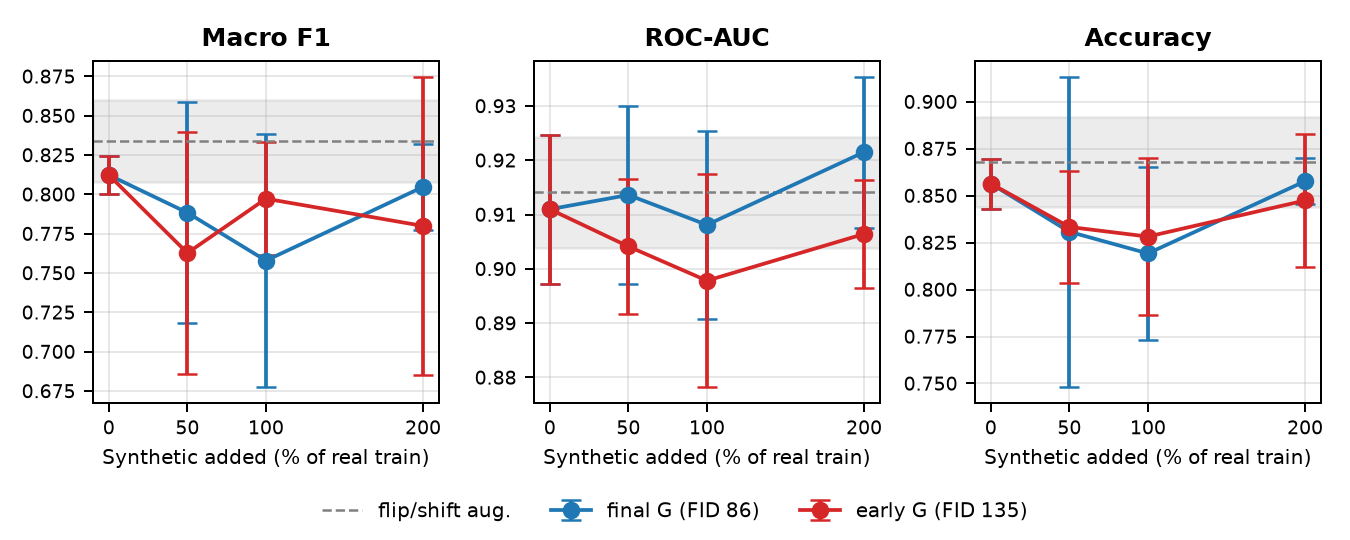
\includegraphics[width=\linewidth]{figures/breast_metrics_vs_ratio.png}
\caption{BreastMNIST: macro F1, ROC-AUC and accuracy against the amount of synthetic data (0\% = real only), for the
final (blue, FID 86) and early (red, FID 135) generator. Error bars: std over 5 seeds. Grey dashed line and band:
classical flip/shift augmentation (mean $\pm$ std).}
\label{fig:ratio}
\end{figure}

\begin{table}[htbp]
\centering
\caption{BreastMNIST per-class recall (mean over 5 seeds; from \texttt{confusion\_matrices.json}). The malignant class is
the clinically important minority class (42 test images).}
\label{tab:recall}
\small
\begin{tabular}{lcc}
\toprule
Setting & Malignant recall & Benign recall \\
\midrule
Real only           & 0.695 $\pm$ 0.085 & 0.916 \\
Real + flip/shift   & \textbf{0.771 $\pm$ 0.069} & 0.904 \\
+50\% GAN (final)   & 0.714 $\pm$ 0.181 & 0.874 \\
+100\% GAN (final)  & 0.662 $\pm$ 0.263 & 0.877 \\
+200\% GAN (final)  & 0.638 $\pm$ 0.106 & 0.939 \\
+100\% GAN (early)  & 0.810 $\pm$ 0.087 & 0.835 \\
GAN class balancing & 0.695 $\pm$ 0.124 & 0.926 \\
\bottomrule
\end{tabular}
\end{table}

\begin{figure}[htbp]
\centering
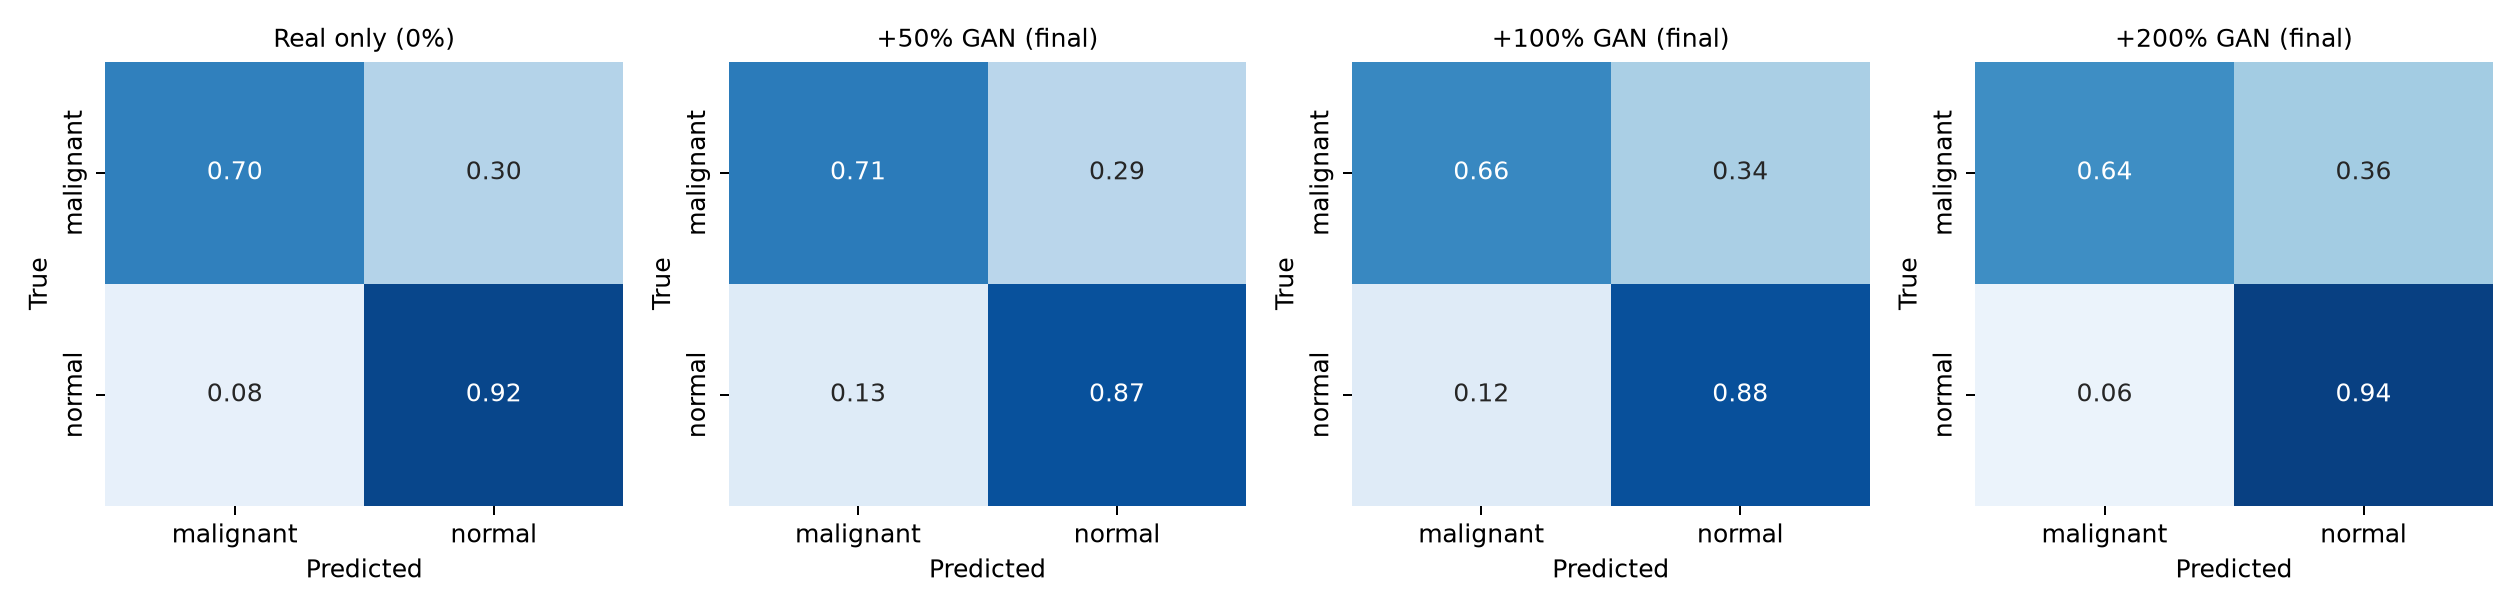
\includegraphics[width=\linewidth]{figures/breast_confusion.png}
\caption{BreastMNIST confusion matrices summed over 5 seeds and normalised per true class (diagonal = per-class recall)
for 0, 50, 100 and 200\% synthetic data from the final generator.}
\label{fig:confusion}
\end{figure}

\noindent The main observations are:
\begin{enumerate}
  \item \textbf{No GAN setting improves macro F1 over real-only training.} Mean F1 changes by between $-0.054$ and
        $+0.006$, and no difference is statistically significant (all $p>0.2$). Accuracy also does not improve
        (best: 0.864 with class balancing vs.\ 0.856).
  \item \textbf{Synthetic data makes training less stable.} The standard deviation of F1 over seeds grows from 0.012
        (real only) to as much as 0.095. With synthetic images in the training set the result depends much more on the
        random seed; e.g.\ one seed of +50\% (final) reached only 0.686 accuracy.
  \item \textbf{Quantity: the effect is not monotonic.} With the final generator, F1 first drops (50\%, 100\%) and then
        recovers almost to the baseline at 200\% (0.805). The +200\% setting gives the \emph{highest AUC} of all
        settings (0.922 vs.\ 0.911), i.e.\ slightly better ranking of cases, but it predicts ``benign'' more often:
        malignant recall falls to 0.638 while benign recall rises to 0.939 (Table~\ref{tab:recall}).
  \item \textbf{Quality matters for AUC.} At every ratio the better generator gives a higher AUC than the early one
        (0.914 vs.\ 0.904, 0.908 vs.\ 0.898, 0.922 vs.\ 0.906). Low-quality images (FID 135) lower AUC below the real-only
        baseline at every ratio. For F1 the picture is mixed and within the seed noise.
  \item \textbf{Classical augmentation is the strongest method.} Random flips and shifts give the best F1 (0.834,
        $+0.022$), the best accuracy (0.868) and raise malignant recall from 0.695 to 0.771 -- at no extra cost and with
        no generator. The difference is not significant at 5 seeds ($p=0.15$), but it is the only consistent positive trend.
  \item \textbf{GAN class balancing is neutral.} Adding 252 synthetic malignant images (to 399 vs.\ 399) leaves F1
        (0.819) and malignant recall (0.695) essentially unchanged: the synthetic minority images did not teach the
        classifier anything about malignant lesions that the 147 real ones did not.
\end{enumerate}

\FloatBarrier
\subsection{Second dataset: PneumoniaMNIST}
PneumoniaMNIST has nine times more real training images (4{,}708). Here the conditional DCGAN produces convincing chest
X-rays (Figure~\ref{fig:pneu_samples}): synthetic \emph{normal} images show clear lung fields and synthetic
\emph{pneumonia} images show hazy, opaque lungs, i.e.\ the class condition is respected. FID against 2{,}000 real training
images is 108.1 for the final and 193.3 for the early generator (real-vs-real reference: 25.3), and only
1.9\% of the generated images are closer to a training image than the closest 5\% of real test images -- fewer than
the 5\% expected for unseen real images, so again there is no memorisation. The quality gap is larger than on
BreastMNIST relative to the reference (108.1 vs.\ 25.3), even though the samples look convincing to the eye.

\begin{figure}[htbp]
\centering
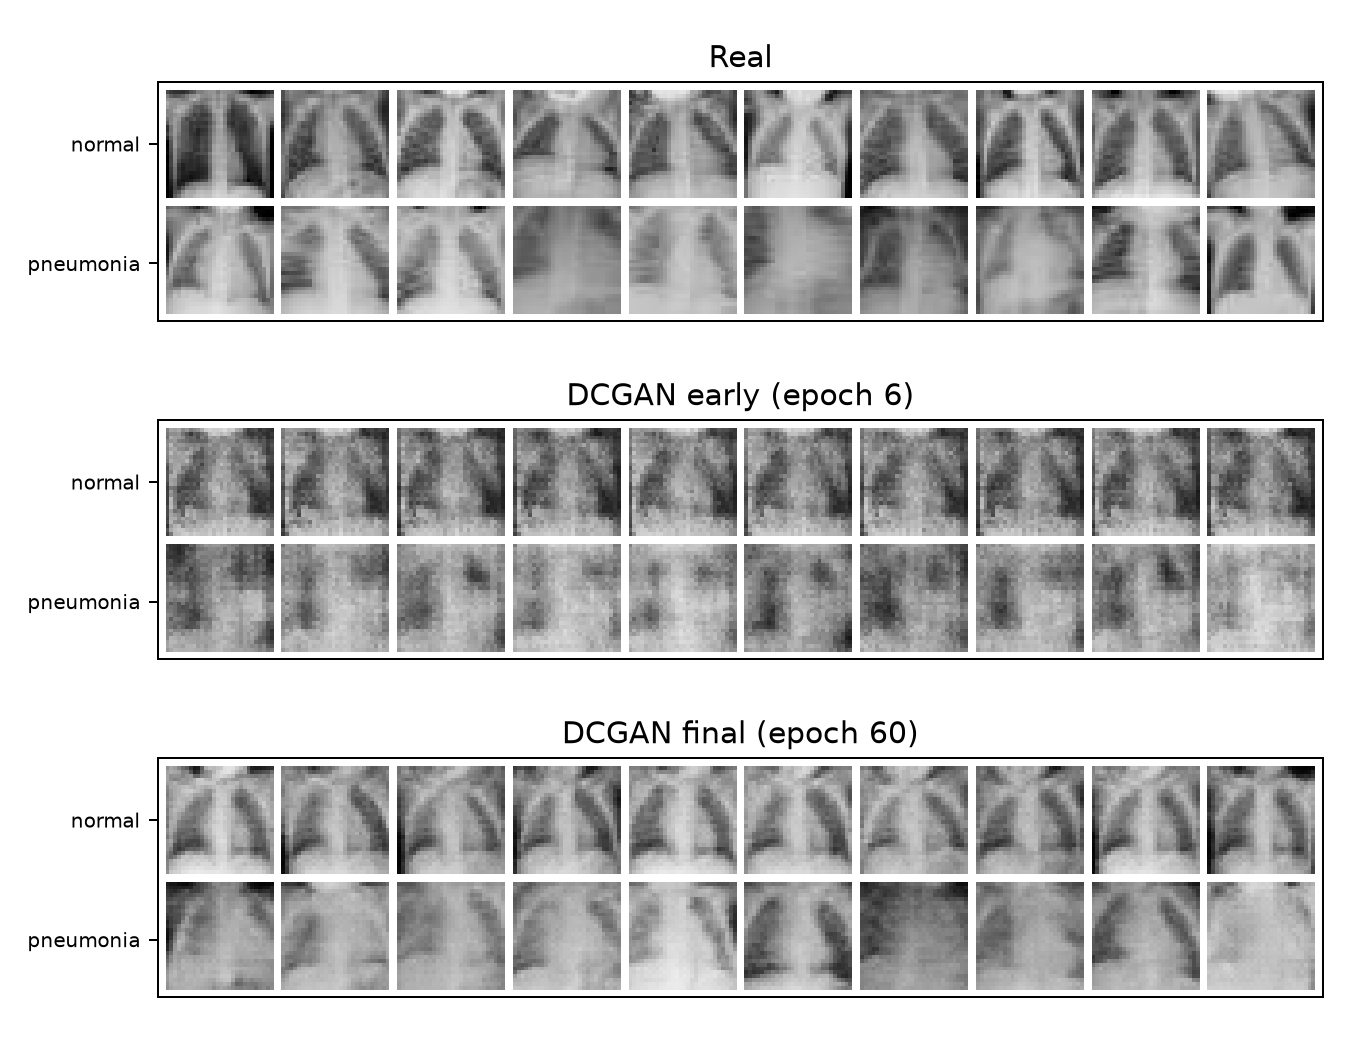
\includegraphics[width=0.9\linewidth]{figures/pneumonia_real_vs_synthetic.png}
\caption{PneumoniaMNIST: real training images (top), early generator after 6 epochs (middle), final generator after 60
epochs (bottom); one row per class.}
\label{fig:pneu_samples}
\end{figure}

\begin{table}[htbp]
\centering
\caption{PneumoniaMNIST, real test set (624 images), mean $\pm$ std over 3 seeds, 15 classifier epochs. $p$: Welch's
$t$-test on per-seed macro F1 vs.\ real only. Normal recall = recall of the minority class \emph{normal}.
Source: \texttt{results/pneumoniamnist/}.}
\label{tab:pneu}
\resizebox{\linewidth}{!}{%
\begin{tabular}{lcccccc}
\toprule
Setting & Accuracy & Macro F1 & AUC & Normal recall & $\Delta$F1 & $p$ \\
\midrule
Real only (0\%)     & \textbf{0.880 $\pm$ 0.017} & \textbf{0.861 $\pm$ 0.021} & 0.973 $\pm$ 0.006 & \textbf{0.691} & --       & --    \\
Real + flip/shift   & 0.808 $\pm$ 0.069 & 0.755 $\pm$ 0.104 & 0.972 $\pm$ 0.010 & 0.489 & $-$0.106 & 0.215 \\
\midrule
+50\% GAN (final)   & 0.860 $\pm$ 0.026 & 0.834 $\pm$ 0.035 & 0.973 $\pm$ 0.005 & 0.634 & $-$0.027 & 0.334 \\
+100\% GAN (final)  & 0.873 $\pm$ 0.006 & 0.853 $\pm$ 0.008 & 0.975 $\pm$ 0.002 & 0.668 & $-$0.008 & 0.573 \\
+200\% GAN (final)  & 0.875 $\pm$ 0.003 & 0.855 $\pm$ 0.004 & \textbf{0.976 $\pm$ 0.002} & 0.671 & $-$0.006 & 0.652 \\
+100\% GAN (early)  & 0.868 $\pm$ 0.005 & 0.845 $\pm$ 0.006 & 0.973 $\pm$ 0.001 & 0.651 & $-$0.016 & 0.317 \\
GAN class balancing & 0.863 $\pm$ 0.015 & 0.838 $\pm$ 0.019 & 0.973 $\pm$ 0.002 & 0.635 & $-$0.023 & 0.240 \\
\bottomrule
\end{tabular}}
\end{table}

\begin{figure}[htbp]
\centering
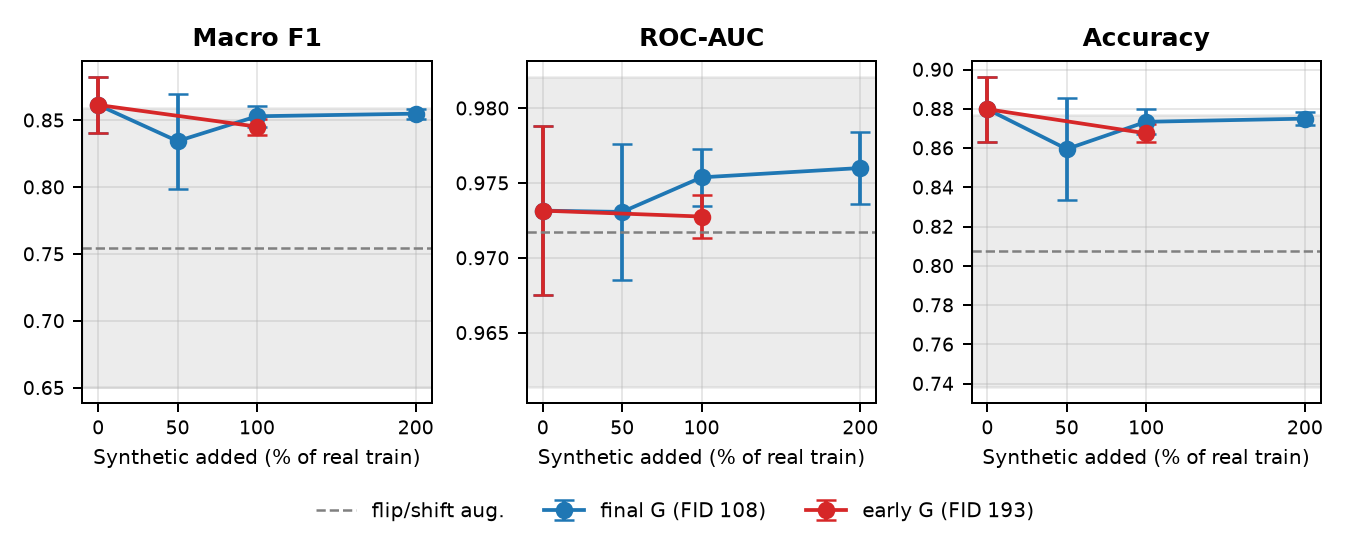
\includegraphics[width=\linewidth]{figures/pneumonia_metrics_vs_ratio.png}
\caption{PneumoniaMNIST: metrics against the amount of synthetic data. Note how the error bars shrink as more synthetic
images are added, while the means stay at the real-only level.}
\label{fig:pneu_ratio}
\end{figure}

\noindent Table~\ref{tab:pneu} and Figure~\ref{fig:pneu_ratio} show the same overall answer as on BreastMNIST, with two
instructive differences:
\begin{enumerate}
  \item \textbf{Again, no F1 gain.} No GAN setting beats the real-only baseline (F1 0.861); differences range from
        $-0.027$ to $-0.006$ and none is significant (all $p>0.2$). The real-only baseline (accuracy 0.880, AUC 0.973)
        is above the MedMNIST v2 ResNet-18 reference (0.854 / 0.944).
  \item \textbf{Synthetic data stabilises training here.} The seed-to-seed standard deviation of F1 falls from 0.021
        (real only) to 0.008 (+100\%) and 0.004 (+200\%), and the +200\% setting has the highest AUC (0.976). With a
        larger real set, the GAN is a better model of the data and its images act as a mild regulariser.
  \item \textbf{Quality still matters.} At +100\%, the final generator beats the early one on every metric (F1 0.853
        vs.\ 0.845, AUC 0.975 vs.\ 0.973, normal recall 0.668 vs.\ 0.651).
  \item \textbf{Classical augmentation hurts on chest X-rays.} Horizontal flipping drops F1 to 0.755 and normal recall to
        0.489. A mirrored chest X-ray puts the heart on the wrong side -- an anatomically impossible image -- whereas a
        mirrored breast ultrasound is still realistic. Augmentation must respect the anatomy of the modality.
  \item \textbf{All models under-detect the normal class.} Pneumonia recall is above 0.99 in every setting, but normal
        recall is only 0.49--0.69, so most errors are normal patients predicted as pneumonia. Neither proportional
        augmentation nor GAN class balancing (normal recall 0.635) fixed this.
\end{enumerate}

% -------------------------------------------------------------------------------------
\FloatBarrier
\section{Discussion}
\textbf{Answer to the research question.} In our setting, adding DCGAN-generated images did \emph{not} improve a CNN
classifier on real test images, on either dataset, at any amount (50--200\%) or quality (FID 86 vs.\ 135). This
differs from the improvement reported by Frid-Adar et al.~\cite{fridadar2018gan}, and we see four reasons in our results.

\begin{enumerate}
  \item \textbf{A GAN cannot add information it never saw.} The generator is trained on the same 546 (or 4{,}708)
        images as the classifier. Our memorisation check shows that it does not copy them, but the samples are
        variations of the same visual content -- with limited diversity (near-duplicate samples, Figure~\ref{fig:nn}).
        New \emph{information} about rare cases (e.g.\ unusual malignant lesions) can only come from new real data.
  \item \textbf{The quality gap acts like label noise.} With FID 86 against a real-vs-real floor of 59, part of the
        synthetic images are not clearly typical of their class. When such images make up a third to two thirds of the
        training set, the classifier partly learns GAN artefacts and ambiguous class boundaries; on BreastMNIST this
        shows up as a lower and less stable F1 at 50--100\%.
  \item \textbf{Quantity helps ranking more than decisions.} At 200\%, AUC is the best of all settings on both datasets
        (0.922 and 0.976), so synthetic images seem to regularise the learned features; but the decision threshold
        shifts towards the majority class (malignant recall 0.638). A threshold tuned on validation data might
        turn this AUC gain into an F1 gain -- a cheap follow-up experiment.
  \item \textbf{Better images help, but not enough.} The final generator beats the early one in AUC at every BreastMNIST
        ratio and on every PneumoniaMNIST metric, so quality clearly matters; the trend suggests that a stronger
        generator (StyleGAN2-ADA, diffusion) is a prerequisite for gains, not an option.
\end{enumerate}

\textbf{Dataset size changes the role of synthetic data.} With 546 images, synthetic data mainly added variance; with
4{,}708 images it reduced variance (std of F1 from 0.021 to 0.004). A GAN trained on more data is a better model of
that data, and its samples then behave like a smooth regulariser rather than noise.

\textbf{Classical augmentation must match the modality.} Simple flips and shifts were the best method for breast
ultrasound (F1 +0.022, malignant recall +0.076) but the worst for chest X-rays (F1 $-0.106$), because a mirrored chest is
anatomically wrong. Domain knowledge matters more than the sophistication of the augmentation method.

\textbf{Why multiple seeds were essential.} With a single seed we could have reported almost any conclusion: individual
BreastMNIST runs of +50\% GAN range from accuracy 0.686 to 0.891. Only the mean over seeds, the standard deviation and the
$t$-test reveal that none of the differences is reliable -- a methodological point that much of the GAN-augmentation
literature does not address.

\textbf{Practical recommendation.} For a small medical dataset, first use modality-appropriate classical augmentation and
report results over several seeds; consider GAN augmentation only with a generator whose FID is close to the real-vs-real
floor, check it for memorisation, and evaluate it against the classical baseline as done here.

\section{Limitations and Future Work}
\begin{itemize}
  \item \textbf{Resolution.} We used 28$\times$28 images to fit a CPU budget; fine lesion details are lost. MedMNIST+ offers
        64--224\,px versions on which both the GAN and the classifier could behave differently.
  \item \textbf{Generator family.} DCGAN is a 2016 architecture. StyleGAN2-ADA or diffusion models produce markedly better
        samples on small datasets and may change the conclusion.
  \item \textbf{Metric mismatch.} FID relies on ImageNet features that are poorly suited to grayscale ultrasound; a
        medical-domain feature extractor would give a more meaningful quality score.
  \item \textbf{Statistics.} Five (three) seeds give a rough estimate of variance; the BreastMNIST test set has only
        42 malignant images, so a single changed prediction moves recall by 2.4 points.
  \item \textbf{Single classifier.} We used one small CNN; a larger or pretrained model may benefit differently from
        synthetic data.
  \item \textbf{No clinical validation.} Synthetic images were not reviewed by radiologists; the system is a research
        prototype, not a diagnostic tool.
\end{itemize}

\section{Conclusion}
We built a complete, reproducible pipeline to test whether GAN-generated images help a classifier trained on a small
medical dataset. A class-conditional DCGAN with DiffAugment-style translation learned realistic-looking breast ultrasound
and chest X-ray images without memorising its training data, and a better generator (lower FID) consistently gave better
classifiers than a worse one. Nevertheless, adding 50--200\% synthetic images did not improve macro F1 on real test
images for either dataset, and no difference was statistically significant over 5 (3) seeds. Synthetic data raised AUC
slightly at 200\% and, on the larger dataset, made training much more stable, while simple flip/shift augmentation was the
best method for ultrasound but harmful for chest X-rays. The answer to ``does synthetic data help?'' is therefore:
\emph{not by itself with a DCGAN at this scale -- quality, dataset size and the choice of baseline decide}.
Future work: higher resolution (MedMNIST+), stronger generators (StyleGAN2-ADA, diffusion), threshold tuning, and
filtering synthetic images by classifier confidence before adding them.

\section*{Code Availability and Demo}
Code, results and instructions: \url{https://github.com/Bhagwati23/GAN-medicalAugmentation}. The package \texttt{ganaug}
contains one module per stage (data, DCGAN, GAN training, augmentation, classifier, FID, experiments, report figures);
\texttt{tests/} checks shapes, determinism and that synthetic images never reach the validation or test sets; a GitHub
Actions workflow runs these tests on every pull request. \texttt{app.py} is a Gradio web app that generates synthetic images
for a chosen class and generator checkpoint, classifies an uploaded or real test image with both the real-only and the
GAN-augmented classifier side by side, and shows the result tables.

\section*{Individual Contributions}
\begin{itemize}
  \item \textbf{Arjun Kadam} (su-24022@sitare.org): synthetic-data augmentation pipeline (issue \#5), integration, testing,
        CI and reproducibility (\#8), demo application, project report (\#9).
  \item \textbf{Bhagwati} (su-24032@sitare.org): conditional DCGAN architecture (\#3), GAN training, checkpoints and samples (\#4), independent re-run of GAN training (reproducibility check);
        repository set-up, issue planning, team workflow, and PR review and merge coordination.
  \item \textbf{Maneesh Sakhwar} (su-24068@sitare.org): dataset selection, loading, exploration notebook and data-leakage tests (\#1); FID/KID evaluation
        and memorisation check (\#6).
  \item \textbf{Anand Singh} (su-24014@sitare.org): CNN baseline (\#2); experiment runs, comparison tables and figures (\#7).
\end{itemize}

.
% Every number comes from results/ in the repository (see the table/figure captions).
% =====================================================================================

\begin{abstract}
Medical image datasets are often small and class-imbalanced, which limits how well deep classifiers can be trained.
We study whether images generated by a Generative Adversarial Network (GAN) can make up for this.
We train a class-conditional DCGAN on the training split of BreastMNIST (546 breast ultrasound images, 27\% malignant)
and add 0, 50, 100 or 200\% synthetic images to the training set of a CNN classifier, which is always evaluated on the
same held-out set of \emph{real} test images. To separate the effect of the \emph{amount} of synthetic data from its
\emph{quality}, we repeat every experiment with an early generator checkpoint (FID 134.9) and the fully trained
generator (FID 86.4; the real-vs-real reference is 59.1), compare against classical flip/shift augmentation and
against GAN-based class balancing, run five random seeds per setting, and test significance with Welch's $t$-test.
The generator learns realistic images without memorising the training set, and the better generator consistently beats
the worse one. Yet no amount of synthetic data improves macro F1 over real-only training (0.812; changes from $-0.054$ to
$+0.006$, none significant), while simple flip/shift augmentation gives the best F1 (0.834). Adding 200\% synthetic images
yields the highest AUC (0.922 vs.\ 0.911) but lowers malignant recall.
A second, nine times larger dataset (PneumoniaMNIST) is used to check whether the conclusion depends on dataset size.
All code, results and an interactive demo are available at \url{https://github.com/Bhagwati23/GAN-medicalAugmentation}.

\vspace{0.5cm}
\noindent
{\em Key Words}: Generative Adversarial Networks, DCGAN, Data Augmentation, Medical Image Classification,
Synthetic Data, MedMNIST, FID.
\end{abstract}
\hrulefill

% -------------------------------------------------------------------------------------
\section{Introduction}
Deep convolutional networks need many labelled examples, but labelled medical images are expensive: they require
expert annotation, are protected by privacy rules, and positive (disease) cases are rare. The usual remedy is
\emph{data augmentation}: creating new training examples from existing ones. Classical augmentation applies simple
geometric or photometric transforms (flips, shifts, rotations, contrast changes)~\cite{shorten2019survey}. Generative
Adversarial Networks (GANs)~\cite{goodfellow2014gan} offer a more ambitious option: learn the distribution of the
training images and sample entirely new ones. Frid-Adar et al.~\cite{fridadar2018gan} reported that GAN-generated
liver-lesion images raised CNN sensitivity and specificity, which made GAN augmentation popular in medical
imaging~\cite{yi2019ganmedical}.

However, a GAN trained on a small dataset only sees the same few hundred images as the classifier. It is therefore not
obvious that its samples add \emph{new information}; they may only add noise, or copies of the training images.
This project asks a precise question:

\begin{quote}
\emph{When a classifier is trained on a small medical dataset, does adding GAN-generated images improve its performance
on real, unseen images -- and how does the gain depend on the amount and on the quality of the synthetic data?}
\end{quote}

\noindent\textbf{Contributions.}
\begin{itemize}
  \item A reproducible pipeline (MedMNIST v2 data, class-conditional DCGAN, augmentation at 0/\allowbreak 50/\allowbreak 100/\allowbreak 200\%, CNN
        classifier, FID/KID evaluation) with strict separation of training, validation and test data.
  \item A two-axis study: \emph{quantity} (four synthetic ratios) $\times$ \emph{quality} (early vs.\ final generator,
        measured by FID and KID), plus two reference points: classical flip/shift augmentation and GAN class balancing.
  \item Statistical care: five seeds per setting, mean $\pm$ standard deviation, Welch's $t$-test against the real-only baseline.
  \item Checks that the generator does not simply memorise the training set (nearest-neighbour distances and latent
        interpolation).
  \item A replication on a second, larger dataset (PneumoniaMNIST) and an interactive web demo.
\end{itemize}

\begin{keybox}{Key findings at a glance}
\begin{itemize}
  \item \textbf{No F1 gain from GAN images} on either dataset at 50, 100 or 200\% synthetic data (BreastMNIST real-only
        F1 0.812 vs.\ 0.758--0.819 with GAN data; none significant, all $p>0.2$).
  \item \textbf{Quality matters:} the better generator (FID 86) beats the early one (FID 135) in AUC at every ratio.
  \item \textbf{200\% synthetic gives the best AUC} on both datasets (0.922 and 0.976) and, on the larger dataset,
        cuts seed-to-seed variance five-fold.
  \item \textbf{No memorisation:} no generated image is closer to a training image than typical unseen real images.
  \item \textbf{Classical augmentation depends on anatomy:} best for breast ultrasound (F1 0.834), harmful for chest
        X-rays (F1 0.755) because mirrored chests are anatomically wrong.
\end{itemize}
\end{keybox}

% -------------------------------------------------------------------------------------
\section{Related Work}
\textbf{GANs and DCGAN.} A GAN~\cite{goodfellow2014gan} trains a generator $G$ to map random noise $z$ to images and a
discriminator $D$ to tell real from generated images; the two are trained against each other. DCGAN~\cite{radford2016dcgan}
gave architectural rules that make this training stable for images: strided (transposed) convolutions instead of pooling,
batch normalisation, ReLU in $G$, LeakyReLU in $D$, Adam with learning rate $2\times10^{-4}$ and $\beta_1=0.5$.
Conditional GANs~\cite{mirza2014cgan} feed the class label to both networks so that images of a chosen class can be requested.

\textbf{GANs with little data.} With few training images the discriminator quickly memorises them and stops giving
useful gradients. DiffAugment~\cite{zhao2020diffaugment} applies the same random, differentiable augmentation to real and
generated images before the discriminator, which strongly improves GANs trained on a few hundred images.

\textbf{GAN augmentation in medical imaging.} Frid-Adar et al.~\cite{fridadar2018gan} generated liver-lesion CT patches
with DCGAN and improved classification from 78.6\% to 85.7\% sensitivity. Reviews~\cite{yi2019ganmedical} report
mixed results in later work, often without multiple seeds or a comparison with classical augmentation -- gaps this
project addresses.

\textbf{Evaluating generated images.} The Fr\'echet Inception Distance (FID)~\cite{heusel2017fid} compares Inception-v3
feature statistics of real and generated images; the Kernel Inception Distance (KID)~\cite{binkowski2018kid} is an
unbiased alternative better suited to small samples. Ravuri and Vinyals~\cite{ravuri2019cas} showed that such scores do not
fully predict how useful samples are for training a classifier -- which is exactly what our classifier experiments measure.

\textbf{MedMNIST.} MedMNIST v2~\cite{yang2023medmnist} provides standardised, pre-split 28$\times$28 biomedical datasets with
benchmark results, which makes our numbers comparable and reproducible.

% -------------------------------------------------------------------------------------
\section{Datasets}
We use two binary datasets from MedMNIST v2~\cite{yang2023medmnist} at their default 28$\times$28 grayscale resolution and
keep the \emph{official} train/validation/test splits (Table~\ref{tab:data}, Fig.~\ref{fig:data}).

\textbf{BreastMNIST} (main dataset) is derived from a breast ultrasound dataset~\cite{aldhabyani2020busi}; the label is
\emph{malignant} (class 0) or \emph{normal/benign} (class 1). With only 546 training images and 27\% malignant cases it is
exactly the small, imbalanced setting in which synthetic data is supposed to help.

\textbf{PneumoniaMNIST} (second dataset) is derived from paediatric chest X-rays~\cite{kermany2018pneumonia}: \emph{normal}
(class 0) vs.\ \emph{pneumonia} (class 1), with 4{,}708 training images (about nine times more). It tells us whether a
conclusion drawn on BreastMNIST changes when real data is more plentiful.

\begin{table}[htbp]
\centering
\caption{Official MedMNIST v2 splits (images per class). Source: \texttt{results/dataset\_stats.json}.}
\label{tab:data}
\begin{tabular}{llrrr}
\toprule
Dataset & Class & Train & Val & Test \\
\midrule
BreastMNIST    & malignant      & 147   & 21  & 42  \\
               & normal/benign  & 399   & 57  & 114 \\
               & \emph{total}   & 546   & 78  & 156 \\
\midrule
PneumoniaMNIST & normal         & 1{,}214 & 135 & 234 \\
               & pneumonia      & 3{,}494 & 389 & 390 \\
               & \emph{total}   & 4{,}708 & 524 & 624 \\
\bottomrule
\end{tabular}
\end{table}

\begin{figure}[htbp]
\centering
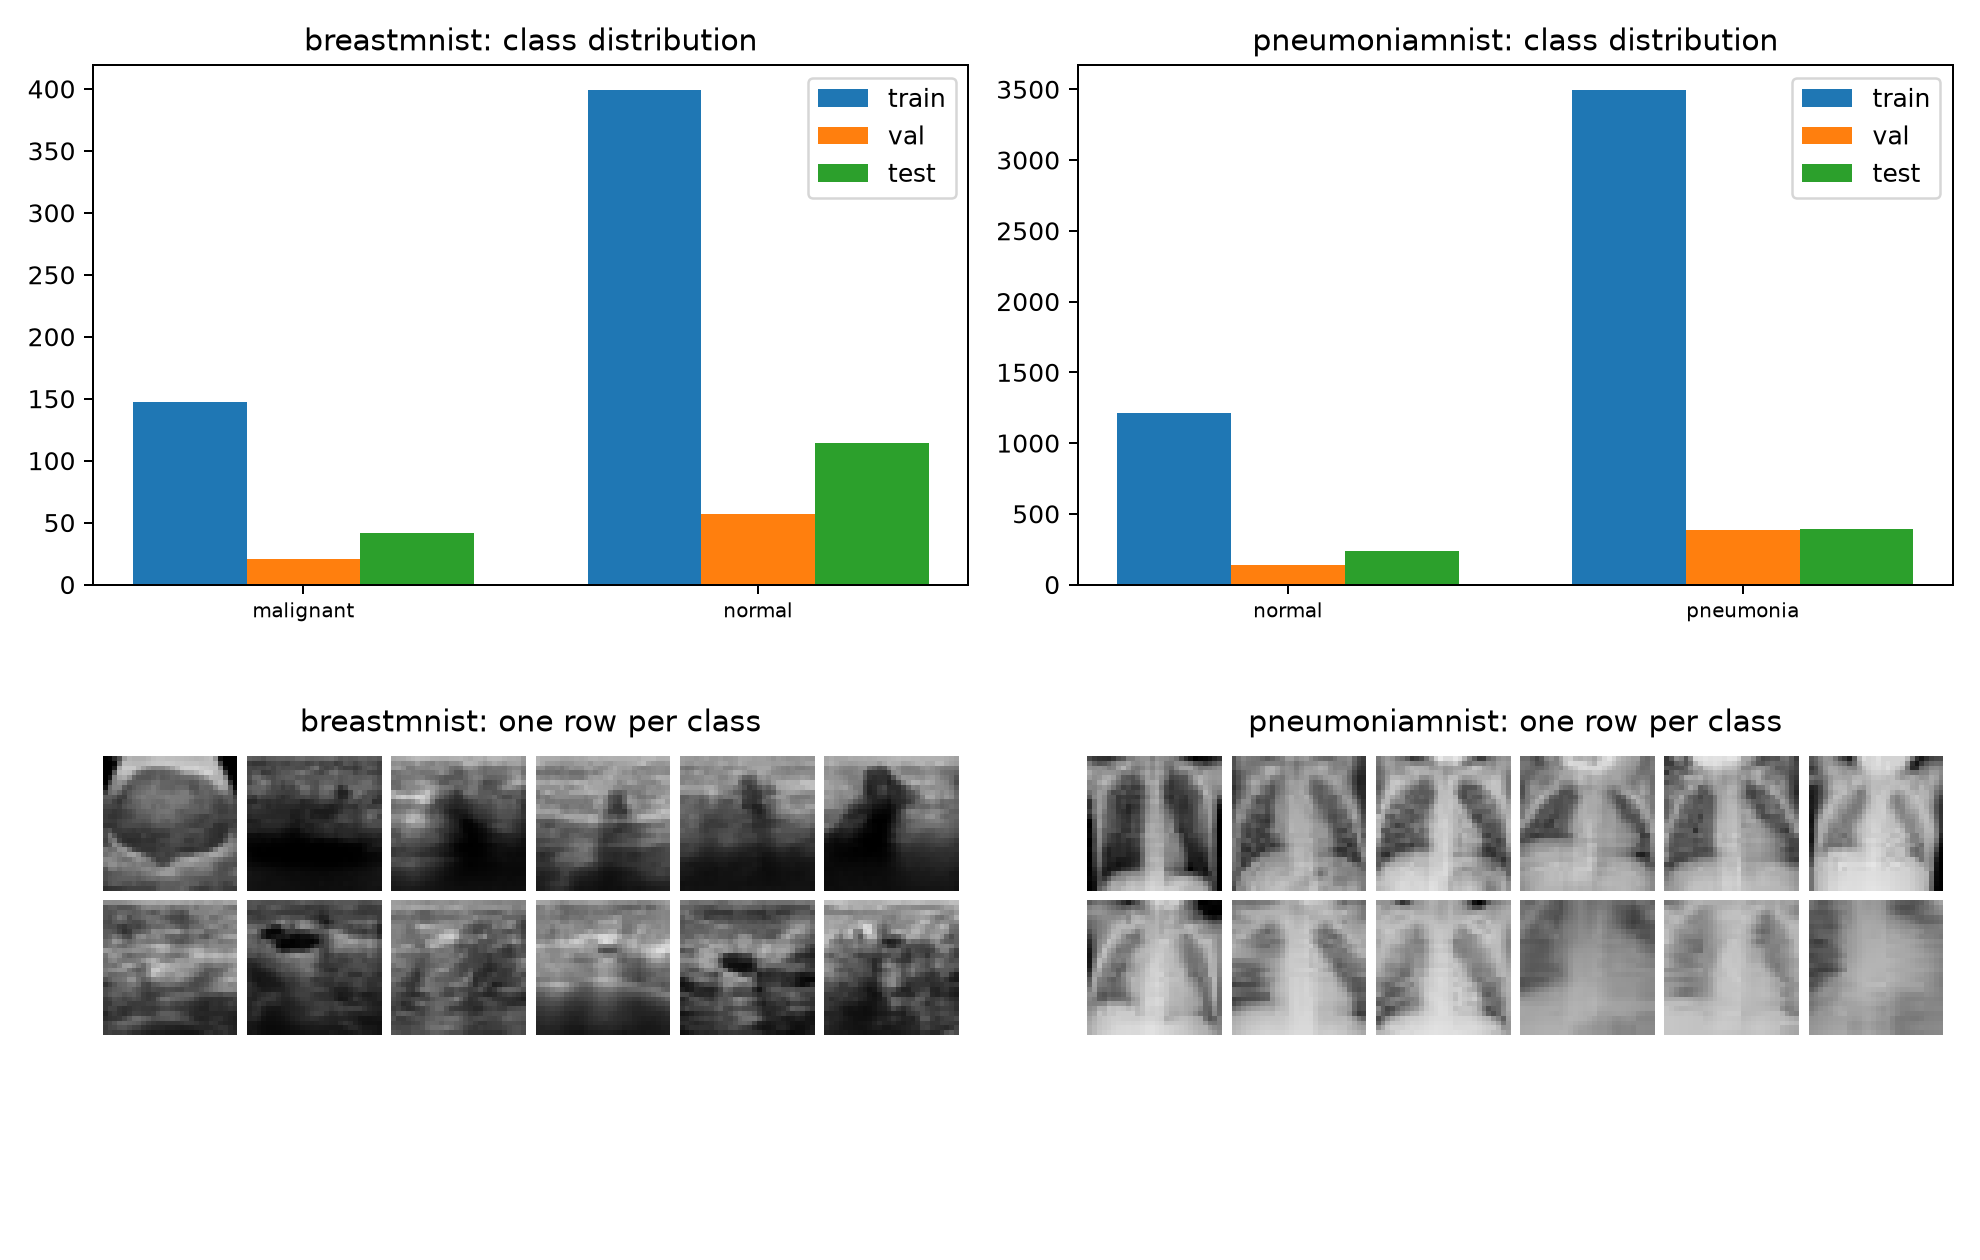
\includegraphics[width=\linewidth]{figures/dataset_overview.png}
\caption{Class distribution per split (top) and training images, one row per class (bottom). Both datasets are imbalanced
(minority class: malignant in BreastMNIST, normal in PneumoniaMNIST).}
\label{fig:data}
\end{figure}

\textbf{Preprocessing and leakage control.} Pixel values are scaled from $[0,255]$ to $[-1,1]$, the output range of the
generator's $\tanh$. The GAN is trained \emph{only} on the training split. Synthetic images are added \emph{only} to the
training split. Validation (used to choose the best epoch) and test (used once, for the final numbers) contain only real
images and are identical in every experiment. These rules are enforced in code and checked by unit tests.

% -------------------------------------------------------------------------------------
\section{Method}

\subsection{Pipeline}
\begin{enumerate}
  \item Train a class-conditional DCGAN on the real training images; save an \emph{early} checkpoint (after 10\% of
        training) and the \emph{final} one.
  \item Score both generators with FID and KID against the real training images, and check for memorisation.
  \item For each setting (Section~\ref{sec:settings}), build a training set of real images plus a controlled number of
        synthetic images, train the CNN classifier with five seeds, and evaluate on the real test set.
  \item Compare every setting with the real-only baseline (mean, standard deviation, Welch's $t$-test).
\end{enumerate}

\subsection{Class-conditional DCGAN}
Table~\ref{tab:gan} lists the architecture. The generator concatenates a 100-dimensional Gaussian noise vector $z$ with a
learned 50-dimensional embedding of the class label $y$, projects it to a $256\times7\times7$ tensor and upsamples it with
two stride-2 transposed convolutions to $28\times28$. The discriminator receives the image together with a learned
$28\times28$ ``label map'' as a second channel, so it judges whether the image is realistic \emph{for that class}.
Following DCGAN~\cite{radford2016dcgan}, weights are initialised from $\mathcal{N}(0,0.02)$, $G$ uses BatchNorm + ReLU and
$D$ uses LeakyReLU(0.2), no pooling layers.

\begin{table}[htbp]
\centering
\caption{Conditional DCGAN architecture (\texttt{ganaug/dcgan.py}). ConvT = transposed convolution, k = kernel, s = stride.}
\label{tab:gan}
\small
\begin{tabular}{ll}
\toprule
\multicolumn{2}{l}{\textbf{Generator} (2.56\,M parameters)} \\
Input & $z\in\mathbb{R}^{100}$ $\oplus$ Embedding$(y)\in\mathbb{R}^{50}$ \\
Linear + BN + ReLU & $150 \rightarrow 256\times7\times7$ \\
ConvT k4 s2 + BN + ReLU & $\rightarrow 128\times14\times14$ \\
ConvT k4 s2 + BN + ReLU & $\rightarrow 64\times28\times28$ \\
Conv k3 s1 + $\tanh$ & $\rightarrow 1\times28\times28$, values in $[-1,1]$ \\
\midrule
\multicolumn{2}{l}{\textbf{Discriminator} (0.43\,M parameters)} \\
Input & image $\oplus$ label map $\rightarrow 2\times28\times28$ \\
Conv k4 s2 + LeakyReLU & $\rightarrow 64\times14\times14$ \\
Conv k4 s2 + BN + LeakyReLU & $\rightarrow 128\times7\times7$ \\
Conv k3 s2 + BN + LeakyReLU & $\rightarrow 256\times4\times4$ \\
Dropout(0.3) + Linear & $\rightarrow$ 1 logit (real/fake) \\
\bottomrule
\end{tabular}
\end{table}

\textbf{Training objective.} With $\sigma$ the sigmoid and $\tilde{x}=T(x)$ a random translation (below), $D$ minimises
\begin{equation}
\mathcal{L}_D = -\,\mathbb{E}_{x,y}\big[\,0.9\log\sigma(D(\tilde{x},y))\big] - \mathbb{E}_{z,y}\big[\log\big(1-\sigma(D(\widetilde{G(z,y)},y))\big)\big],
\end{equation}
and $G$ minimises the non-saturating loss $\mathcal{L}_G = -\,\mathbb{E}_{z,y}\big[\log\sigma(D(\widetilde{G(z,y)},y))\big]$.
Two additions help with only 546 training images:
(i) \emph{one-sided label smoothing}: the target for real images is 0.9 instead of 1, so $D$ does not become over-confident;
(ii) \emph{DiffAugment-style translation}~\cite{zhao2020diffaugment}: every real and generated image is shifted by a random
$-2\ldots2$ pixels (edge-replicate padding) before it is shown to $D$, which keeps $D$ from memorising the training images.
Both networks use Adam ($2\times10^{-4}$, $\beta=(0.5,0.999)$), batch size 64.

\subsection{Augmentation protocol}
\label{sec:aug}
For a ratio $r\in\{0, 0.5, 1, 2\}$ we add $\mathrm{round}(r\cdot n_c)$ synthetic images of each class $c$, where $n_c$ is
the number of real training images of class $c$. This keeps the real class ratio (for BreastMNIST: $+50\%$ = 274,
$+100\%$ = 546, $+200\%$ = 1{,}092 synthetic images). For each generator we sample one fixed pool of synthetic images
(fixed seed) and every ratio takes the first $k$ images of each class, so the sets are \emph{nested}
($50\% \subset 100\% \subset 200\%$): differences between ratios come from the amount of data, not from a luckier draw.
In the \emph{class-balancing} setting we instead add only minority-class images until both classes have the same size
(BreastMNIST: 252 synthetic malignant images, giving 399 vs.\ 399).

\subsection{Classifier}
All settings use the same CNN (\texttt{ganaug/cnn.py}, 0.29\,M parameters): three blocks of
[Conv3$\times$3--BN--ReLU]$\times$2 + MaxPool with 32, 64 and 128 channels ($28\to14\to7\to3$), global average pooling,
dropout 0.3 and a linear layer. It is trained with cross-entropy, AdamW (learning rate $10^{-3}$, weight decay $10^{-4}$),
a cosine learning-rate schedule and batch size 64. After each epoch we compute the validation ROC-AUC and keep the weights
with the best value (model selection on validation, never on test). The model is deliberately small: the dataset is tiny
and all experiments ran on a CPU. Our real-only baseline (Section~\ref{sec:results}) is in line with the ResNet-18 results
reported by MedMNIST v2~\cite{yang2023medmnist} (BreastMNIST, 28$\times$28: accuracy 0.863, AUC 0.901).

\subsection{Evaluation}
\textbf{Classifier metrics} (real test set): accuracy; \emph{macro} precision, recall and F1 (each class weighted
equally, so missing the minority class is penalised; macro recall equals balanced accuracy); ROC-AUC (threshold-free
ranking quality); and confusion matrices. Macro F1 is our main metric because accuracy can look good on imbalanced data
by mostly predicting the majority class.

\textbf{Image quality.} FID and KID are computed with \texttt{torch-fidelity} between the real training images and the
same number of generated images with the same class ratio (images converted to 3-channel uint8 and resized to
299$\times$299 for Inception-v3). Because 28$\times$28 grayscale ultrasound images are very different from ImageNet photos,
absolute FID values are not comparable to natural-image papers; we therefore also report FID between the real training and
real test images as a \emph{reference floor}.

\textbf{Memorisation check.} For every generated image we find the closest real training image (pixel $L_2$ distance) and
compare these distances with the same distances for real \emph{test} images, which are realistic but unseen. A generator
that copies training images would produce many samples closer to the training set than almost any real test image; we
report the fraction of generated images closer than the 5th percentile of the test distances (about 0.05 is expected if
there is no copying).

\textbf{Statistics.} Each setting is trained with seeds 0--4 (BreastMNIST) or 0--2 (PneumoniaMNIST); we report mean
$\pm$ standard deviation and a two-sided Welch's $t$-test of the per-seed macro F1 against the real-only baseline.

% -------------------------------------------------------------------------------------
\section{Experimental Setup}
\label{sec:settings}
\begin{table}[htbp]
\centering
\caption{Experiment settings. Only the training set changes; the CNN, its hyper-parameters, and the validation and test
sets are identical everywhere.}
\label{tab:settings}
\small
\begin{tabular}{lp{5.2cm}}
\toprule
Setting & Training data \\
\midrule
Real only (0\%) & real training images (baseline) \\
Real + flip/shift & real images, random horizontal flip and $\pm2$\,px shift on the fly \\
+50/100/200\% GAN (final) & real + synthetic from the final generator \\
+50/100/200\% GAN (early) & real + synthetic from the early generator \\
GAN class balancing & real + synthetic minority-class images until classes are equal \\
\bottomrule
\end{tabular}
\end{table}

\begin{table}[htbp]
\centering
\caption{Training configuration.}
\label{tab:hparams}
\small
\begin{tabular}{lll}
\toprule
 & BreastMNIST & PneumoniaMNIST \\
\midrule
GAN epochs (updates)       & 300 (2{,}400) & 60 (4{,}380) \\
Early checkpoint           & epoch 30      & epoch 6 \\
Classifier epochs          & 40            & 15 \\
Seeds per setting          & 5             & 3 \\
Settings run               & all 9         & 7 (no early 50/200\%) \\
FID sample size            & 546           & 2{,}000 (random subset) \\
\bottomrule
\end{tabular}
\end{table}

All experiments ran on a laptop CPU with PyTorch. Table~\ref{tab:settings} lists the settings and Table~\ref{tab:hparams}
the configuration. Because PneumoniaMNIST is nine times larger, we used fewer classifier epochs, seeds and settings for it.
Everything is reproduced by \texttt{bash run\_all.sh}.

% -------------------------------------------------------------------------------------
\FloatBarrier
\section{Results}
\label{sec:results}

\subsection{Quality of the synthetic images}
\textbf{Training dynamics.} Figure~\ref{fig:losses} shows that GAN training on BreastMNIST stayed balanced for all 300
epochs: the discriminator loss stays close to $2\ln 2\approx1.39$ (the value when $D$ cannot separate real from fake), and
at the end $D$ assigns on average 0.46 to real and 0.44 to generated images. There is no sign of mode collapse (where
$D(G(z))$ would drop to 0 and all samples would look alike) or of $D$ winning outright.

\textbf{Reproducibility of GAN training.} The GAN training was run twice, independently, on two different laptops with
the same code, configuration and seed: run~1 produced the generators used for every experiment in this report, and run~2
(by Bhagwati, committed as the training log in \texttt{results/}) checks that training can be repeated. Averaged over the
last 10\% of epochs, the two runs agree closely: BreastMNIST discriminator loss 1.371 vs.\ 1.377, $D(x)$ 0.459 vs.\ 0.456
and $D(G(z))$ 0.441 vs.\ 0.444; PneumoniaMNIST discriminator loss 1.376 vs.\ 1.377, $D(x)$ 0.455 vs.\ 0.456. Bit-exact
equality is not expected, because CPU floating-point operations are not deterministic across machines and library
versions, but the training reaches the same balanced state.

\begin{figure}[htbp]
\centering
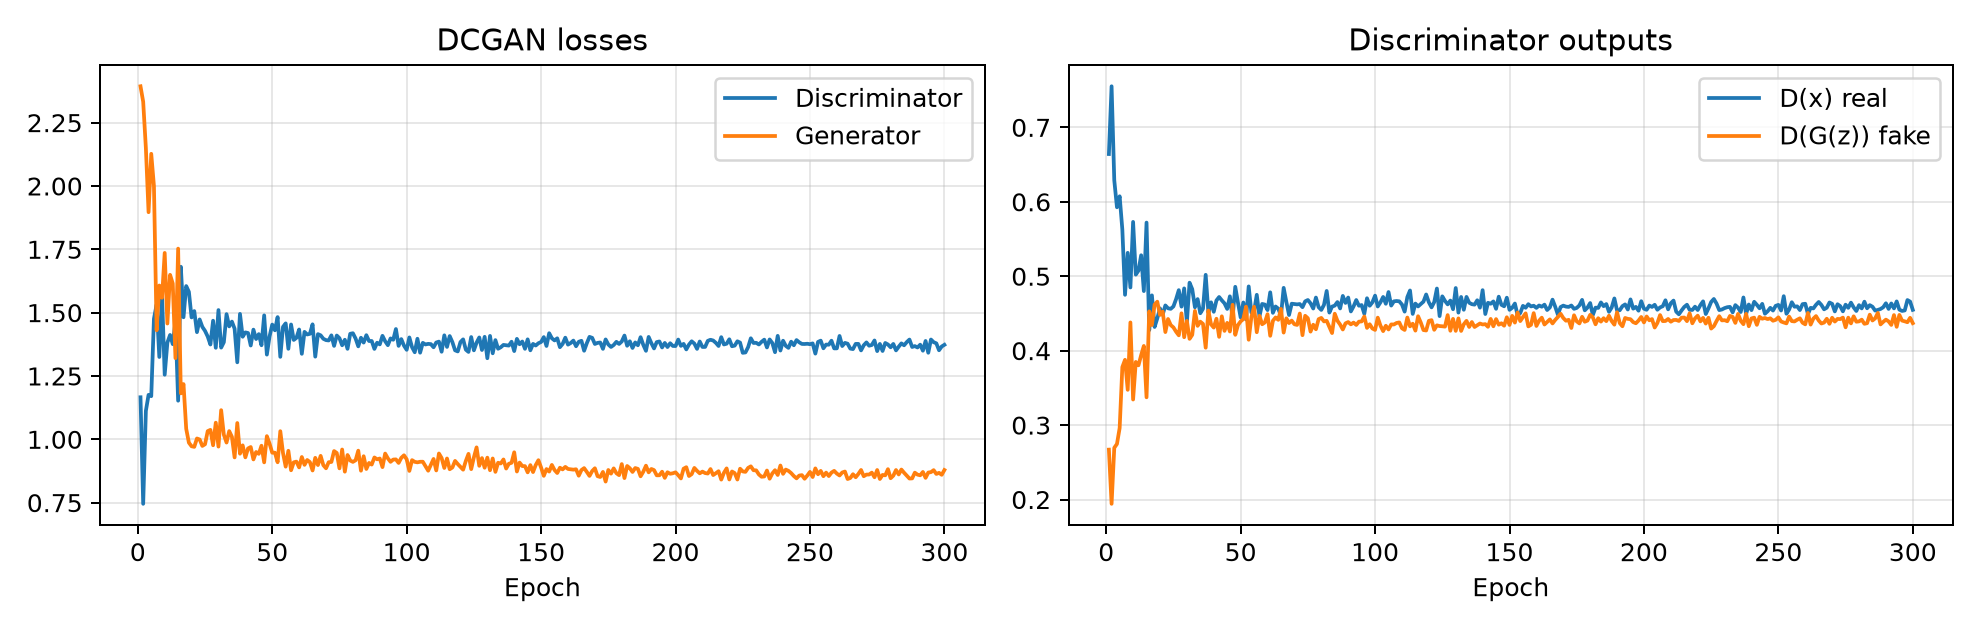
\includegraphics[width=\linewidth]{figures/breast_gan_losses.png}
\caption{DCGAN training on BreastMNIST. Left: losses. Right: mean discriminator output for real ($D(x)$) and generated
($D(G(z))$) images; both stay close to 0.5, i.e.\ a balanced adversarial game. Source: \texttt{results/breastmnist/report\_run/gan\_losses.csv} (run~1).}
\label{fig:losses}
\end{figure}

\textbf{Visual quality.} Figure~\ref{fig:samples} compares real images with samples from both generators. After 30 epochs
the generator only reproduces the global layout (bright tissue at the top, dark region at the bottom) with heavy noise.
After 300 epochs the samples contain lesion-like dark regions and ultrasound speckle texture; synthetic \emph{malignant}
images tend to show larger, darker, irregular masses, matching the real malignant row. Small checkerboard artefacts from
the transposed convolutions remain.

\begin{figure}[htbp]
\centering
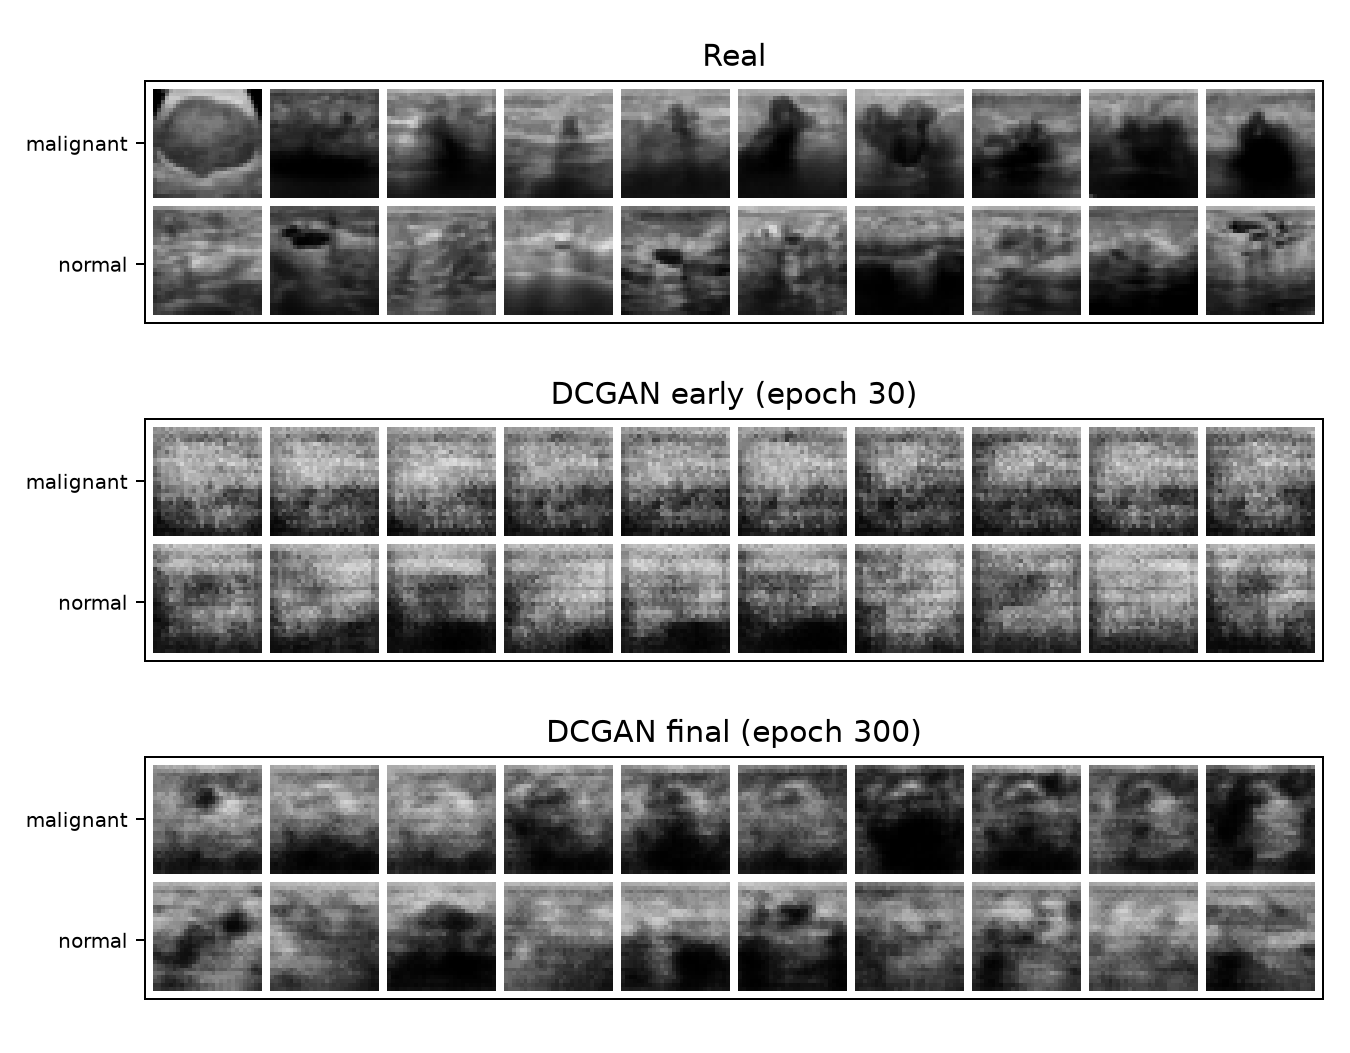
\includegraphics[width=0.9\linewidth]{figures/breast_real_vs_synthetic.png}
\caption{BreastMNIST: real training images (top), early generator after 30 epochs (middle) and final generator after 300
epochs (bottom); one row per class.}
\label{fig:samples}
\end{figure}

\textbf{FID and KID.} Table~\ref{tab:fid} quantifies the quality difference. The final generator reduces FID from 134.9 to
86.4 and KID by about half, but a gap to the real-vs-real reference (59.1) remains: the synthetic distribution is
clearly closer to the real one, yet not identical.

\begin{table}[htbp]
\centering
\caption{Image quality on BreastMNIST (546 images per set; lower is better). Source: \texttt{results/breastmnist/fid.json}.}
\label{tab:fid}
\small
\begin{tabular}{lrr}
\toprule
Compared with real training images & FID & KID \\
\midrule
Real test images (reference floor)   & 59.1  & 0.0004 \\
Early generator (epoch 30)           & 134.9 & 0.1220 \\
Final generator (epoch 300)          & 86.4  & 0.0670 \\
\bottomrule
\end{tabular}
\end{table}

\textbf{No memorisation.} The median distance from a generated image to its nearest training image is 6.33 (final) and
6.96 (early), larger than the 5.52 measured for real test images, and \emph{none} of the generated images is closer to a
training image than the closest 5\% of real test images (fraction 0.00 for both generators). Figure~\ref{fig:nn} shows
generated images next to their nearest training images: they share style but are not copies. The same figure also
shows a weakness: the first two generated images are almost identical to each other, a sign of \emph{limited diversity}
(partial mode collapse) -- the generator does not copy training images, but it also covers fewer distinct variations
than the real data. The latent interpolation in
Figure~\ref{fig:interp} changes smoothly from one image to another, which indicates that the generator learned a continuous
image distribution rather than a lookup table of training images.

\begin{figure}[htbp]
\centering
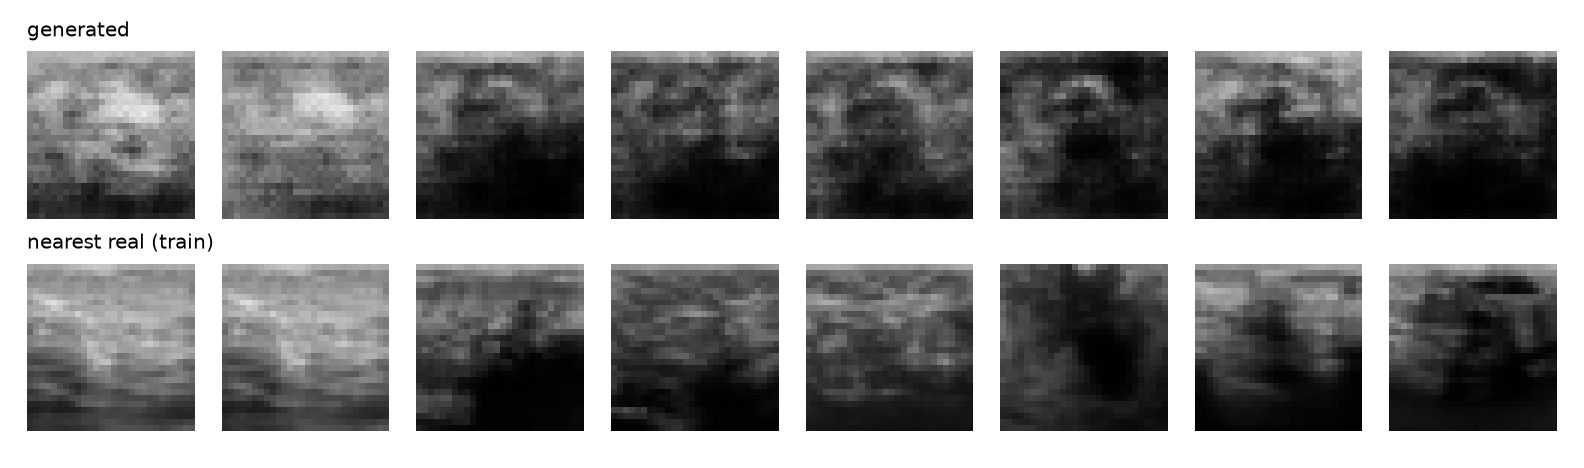
\includegraphics[width=\linewidth]{figures/breast_nearest_neighbours.png}
\caption{Top: images from the final generator. Bottom: the closest real training image to each (pixel $L_2$). Similar
style, different content: the generator does not copy training images. The first two samples are near-duplicates of
each other, showing limited sample diversity.}
\label{fig:nn}
\end{figure}

\begin{figure}[htbp]
\centering
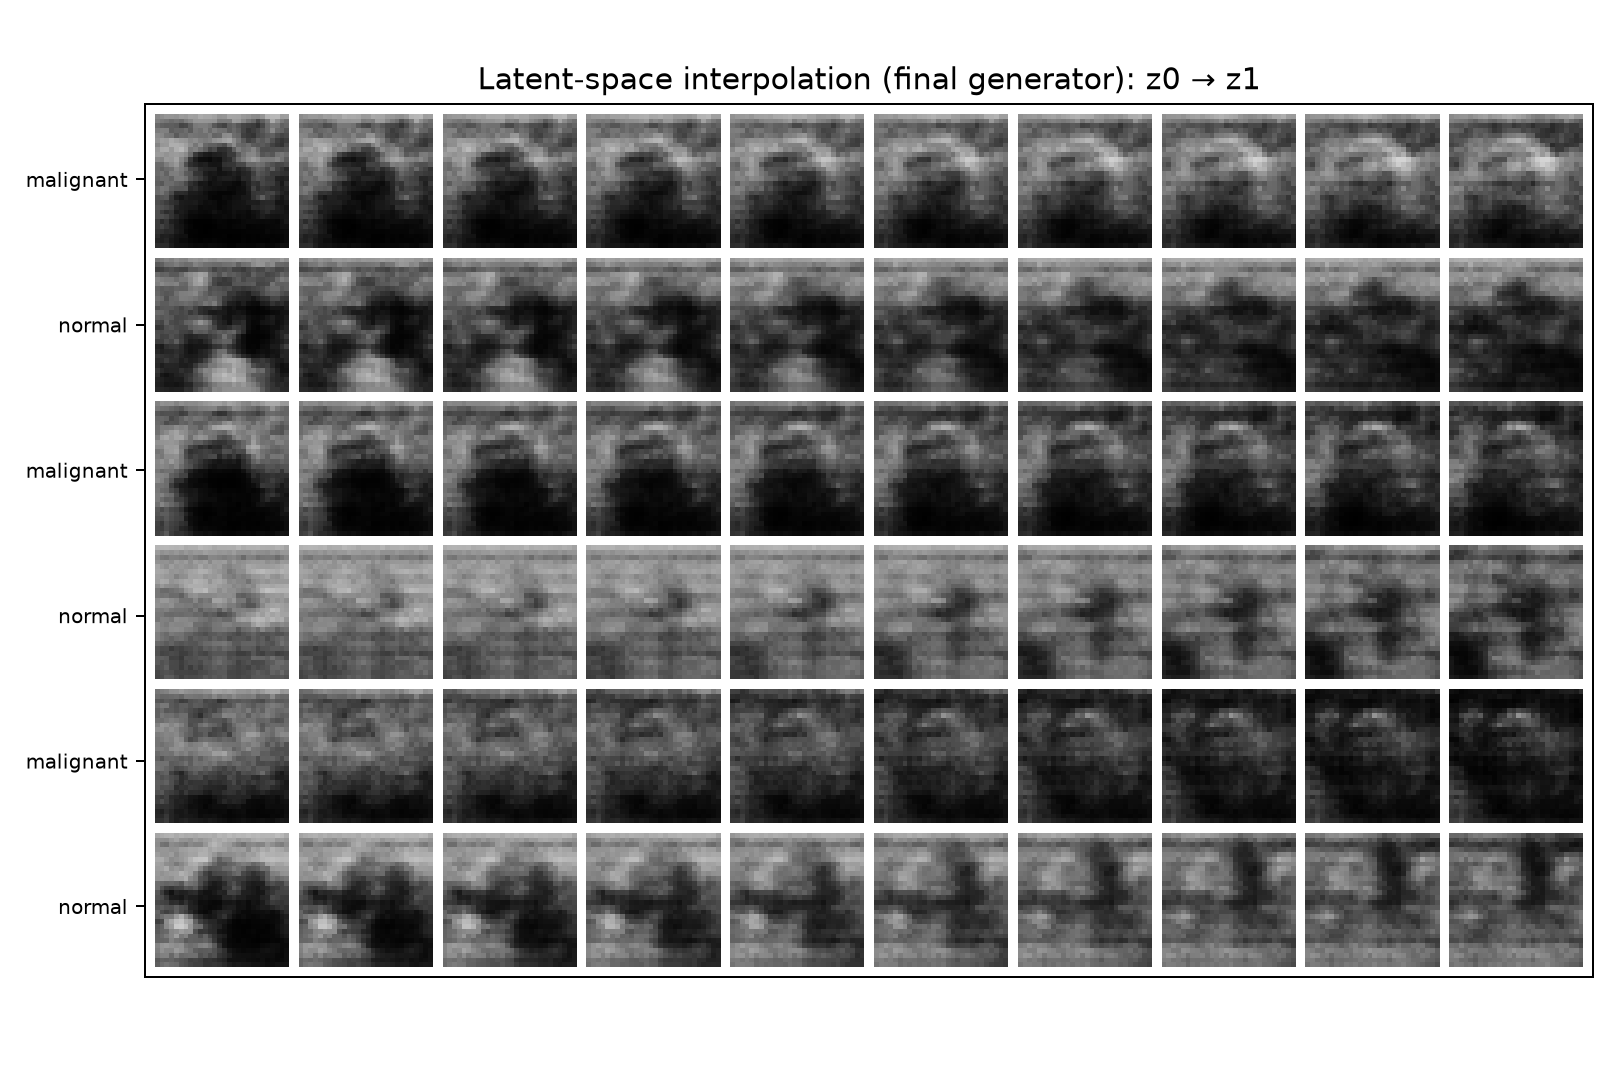
\includegraphics[width=0.85\linewidth]{figures/breast_interpolation.png}
\caption{Linear interpolation between two noise vectors $z_0\to z_1$ (final generator, class fixed per row). Smooth
transitions indicate a continuous learned distribution.}
\label{fig:interp}
\end{figure}

% -------------------------------------------------------------------------------------
\subsection{Does synthetic data help the classifier? (BreastMNIST)}
Table~\ref{tab:breast} and Figure~\ref{fig:ratio} give the main result; Table~\ref{tab:recall} breaks recall down by class.
Our real-only baseline (accuracy 0.856, AUC 0.911) matches the ResNet-18 reference of MedMNIST v2 (0.863 / 0.901), so the
comparison starts from a sound baseline.

\begin{table}[htbp]
\centering
\caption{BreastMNIST, real test set (156 images), mean $\pm$ std over 5 seeds. $\Delta$F1: change in mean macro F1 vs.\
real only; $p$: Welch's $t$-test on per-seed F1 vs.\ real only. Source: \texttt{results/breastmnist/results\_table.md}.}
\label{tab:breast}
\resizebox{\linewidth}{!}{%
\begin{tabular}{lccccccc}
\toprule
Setting & Accuracy & Precision & Recall & Macro F1 & AUC & $\Delta$F1 & $p$ \\
\midrule
Real only (0\%)      & 0.856 $\pm$ 0.013 & 0.829 $\pm$ 0.028 & 0.806 $\pm$ 0.023 & 0.812 $\pm$ 0.012 & 0.911 $\pm$ 0.014 & --     & --    \\
Real + flip/shift    & 0.868 $\pm$ 0.024 & 0.835 $\pm$ 0.031 & 0.837 $\pm$ 0.028 & \textbf{0.834 $\pm$ 0.026} & 0.914 $\pm$ 0.010 & +0.022 & 0.150 \\
\midrule
+50\% GAN (final)    & 0.831 $\pm$ 0.083 & 0.827 $\pm$ 0.059 & 0.794 $\pm$ 0.045 & 0.788 $\pm$ 0.070 & 0.914 $\pm$ 0.016 & $-$0.024 & 0.491 \\
+100\% GAN (final)   & 0.819 $\pm$ 0.046 & 0.816 $\pm$ 0.063 & 0.770 $\pm$ 0.089 & 0.758 $\pm$ 0.080 & 0.908 $\pm$ 0.017 & $-$0.054 & 0.206 \\
+200\% GAN (final)   & 0.858 $\pm$ 0.012 & 0.840 $\pm$ 0.024 & 0.788 $\pm$ 0.040 & 0.805 $\pm$ 0.027 & \textbf{0.922 $\pm$ 0.014} & $-$0.008 & 0.592 \\
\midrule
+50\% GAN (early)    & 0.833 $\pm$ 0.030 & 0.830 $\pm$ 0.046 & 0.758 $\pm$ 0.085 & 0.763 $\pm$ 0.077 & 0.904 $\pm$ 0.012 & $-$0.050 & 0.225 \\
+100\% GAN (early)   & 0.828 $\pm$ 0.042 & 0.792 $\pm$ 0.032 & 0.822 $\pm$ 0.021 & 0.797 $\pm$ 0.036 & 0.898 $\pm$ 0.020 & $-$0.015 & 0.417 \\
+200\% GAN (early)   & 0.847 $\pm$ 0.036 & 0.842 $\pm$ 0.031 & 0.775 $\pm$ 0.097 & 0.780 $\pm$ 0.095 & 0.906 $\pm$ 0.010 & $-$0.032 & 0.490 \\
\midrule
GAN class balancing  & 0.864 $\pm$ 0.019 & 0.838 $\pm$ 0.013 & 0.811 $\pm$ 0.051 & 0.819 $\pm$ 0.039 & 0.916 $\pm$ 0.018 & +0.006 & 0.742 \\
\bottomrule
\end{tabular}}
\end{table}

\begin{figure}[htbp]
\centering
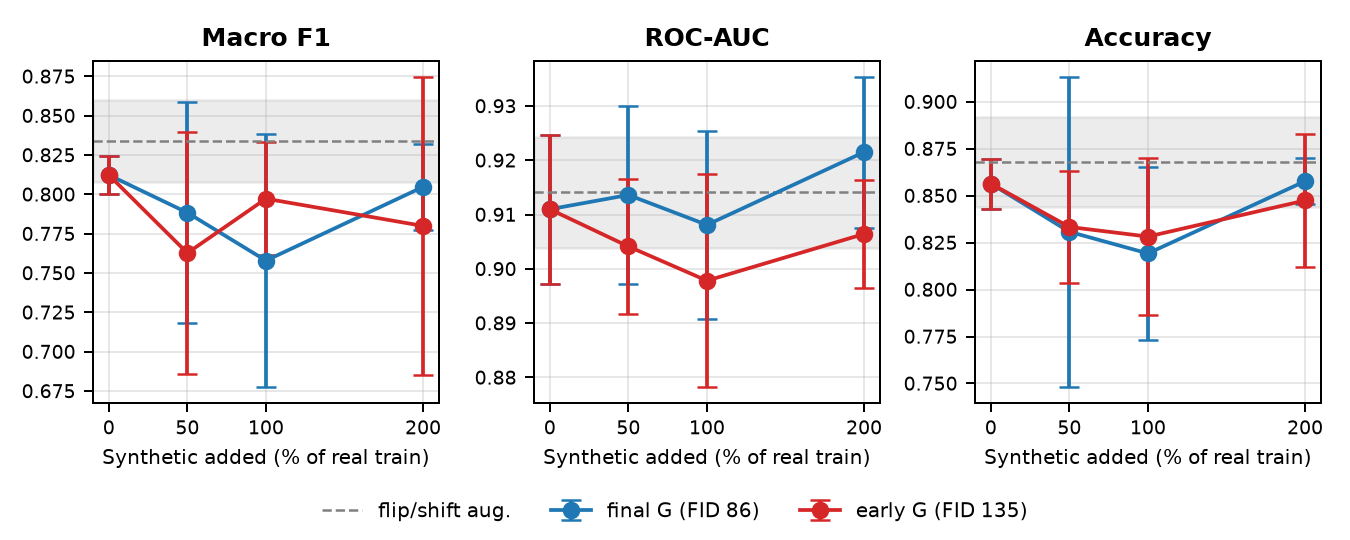
\includegraphics[width=\linewidth]{figures/breast_metrics_vs_ratio.png}
\caption{BreastMNIST: macro F1, ROC-AUC and accuracy against the amount of synthetic data (0\% = real only), for the
final (blue, FID 86) and early (red, FID 135) generator. Error bars: std over 5 seeds. Grey dashed line and band:
classical flip/shift augmentation (mean $\pm$ std).}
\label{fig:ratio}
\end{figure}

\begin{table}[htbp]
\centering
\caption{BreastMNIST per-class recall (mean over 5 seeds; from \texttt{confusion\_matrices.json}). The malignant class is
the clinically important minority class (42 test images).}
\label{tab:recall}
\small
\begin{tabular}{lcc}
\toprule
Setting & Malignant recall & Benign recall \\
\midrule
Real only           & 0.695 $\pm$ 0.085 & 0.916 \\
Real + flip/shift   & \textbf{0.771 $\pm$ 0.069} & 0.904 \\
+50\% GAN (final)   & 0.714 $\pm$ 0.181 & 0.874 \\
+100\% GAN (final)  & 0.662 $\pm$ 0.263 & 0.877 \\
+200\% GAN (final)  & 0.638 $\pm$ 0.106 & 0.939 \\
+100\% GAN (early)  & 0.810 $\pm$ 0.087 & 0.835 \\
GAN class balancing & 0.695 $\pm$ 0.124 & 0.926 \\
\bottomrule
\end{tabular}
\end{table}

\begin{figure}[htbp]
\centering
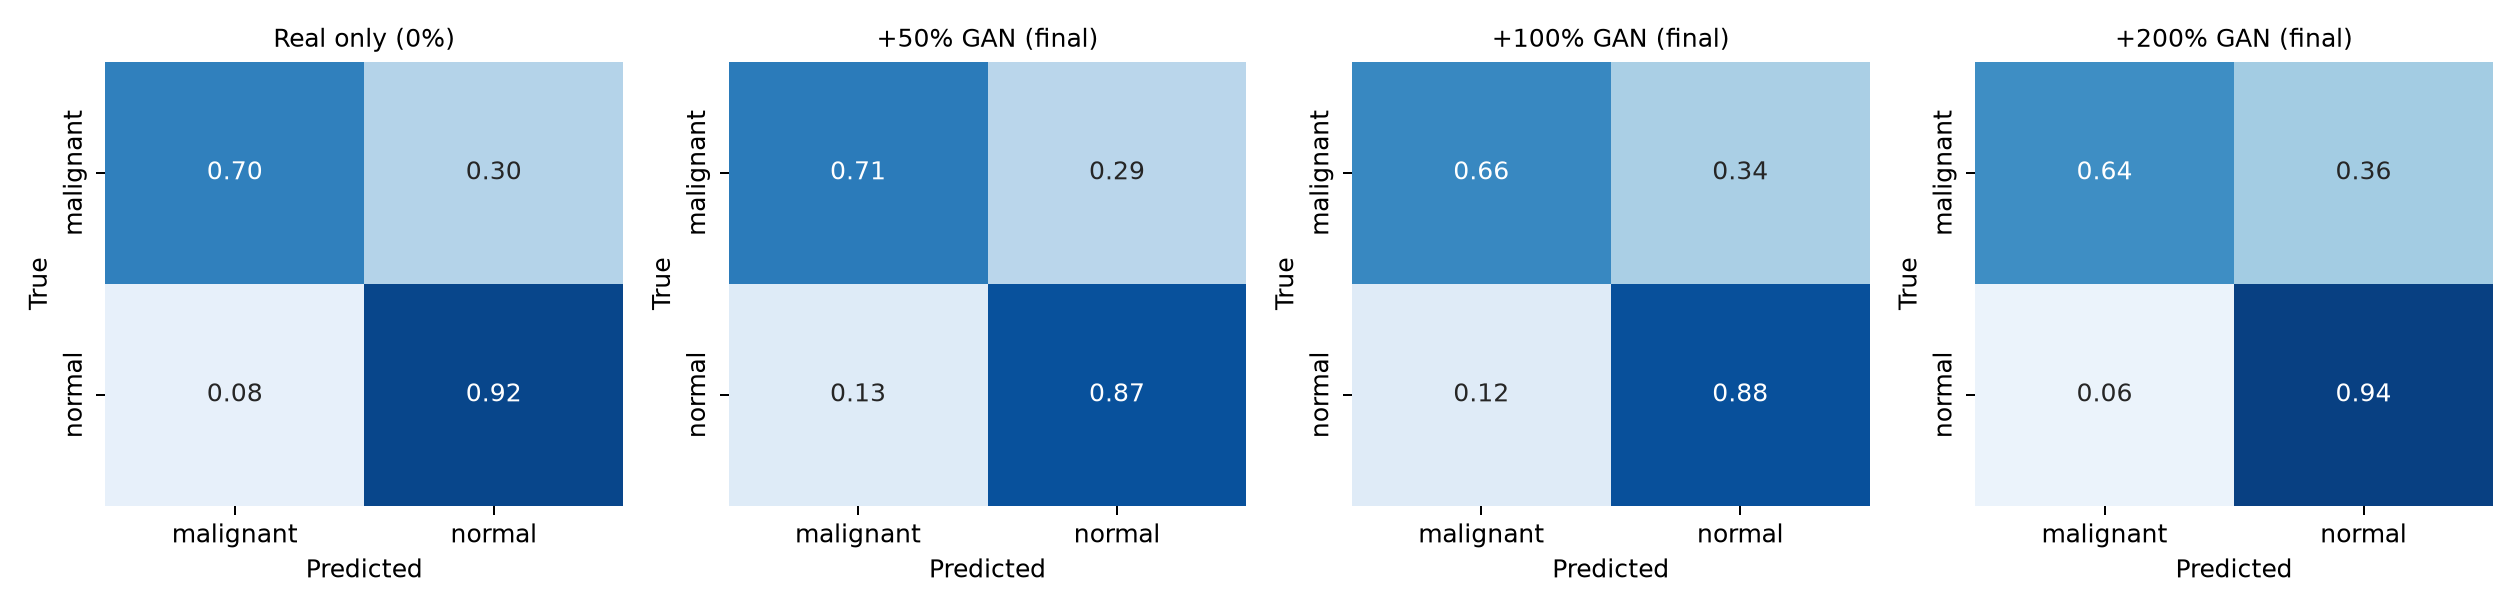
\includegraphics[width=\linewidth]{figures/breast_confusion.png}
\caption{BreastMNIST confusion matrices summed over 5 seeds and normalised per true class (diagonal = per-class recall)
for 0, 50, 100 and 200\% synthetic data from the final generator.}
\label{fig:confusion}
\end{figure}

\noindent The main observations are:
\begin{enumerate}
  \item \textbf{No GAN setting improves macro F1 over real-only training.} Mean F1 changes by between $-0.054$ and
        $+0.006$, and no difference is statistically significant (all $p>0.2$). Accuracy also does not improve
        (best: 0.864 with class balancing vs.\ 0.856).
  \item \textbf{Synthetic data makes training less stable.} The standard deviation of F1 over seeds grows from 0.012
        (real only) to as much as 0.095. With synthetic images in the training set the result depends much more on the
        random seed; e.g.\ one seed of +50\% (final) reached only 0.686 accuracy.
  \item \textbf{Quantity: the effect is not monotonic.} With the final generator, F1 first drops (50\%, 100\%) and then
        recovers almost to the baseline at 200\% (0.805). The +200\% setting gives the \emph{highest AUC} of all
        settings (0.922 vs.\ 0.911), i.e.\ slightly better ranking of cases, but it predicts ``benign'' more often:
        malignant recall falls to 0.638 while benign recall rises to 0.939 (Table~\ref{tab:recall}).
  \item \textbf{Quality matters for AUC.} At every ratio the better generator gives a higher AUC than the early one
        (0.914 vs.\ 0.904, 0.908 vs.\ 0.898, 0.922 vs.\ 0.906). Low-quality images (FID 135) lower AUC below the real-only
        baseline at every ratio. For F1 the picture is mixed and within the seed noise.
  \item \textbf{Classical augmentation is the strongest method.} Random flips and shifts give the best F1 (0.834,
        $+0.022$), the best accuracy (0.868) and raise malignant recall from 0.695 to 0.771 -- at no extra cost and with
        no generator. The difference is not significant at 5 seeds ($p=0.15$), but it is the only consistent positive trend.
  \item \textbf{GAN class balancing is neutral.} Adding 252 synthetic malignant images (to 399 vs.\ 399) leaves F1
        (0.819) and malignant recall (0.695) essentially unchanged: the synthetic minority images did not teach the
        classifier anything about malignant lesions that the 147 real ones did not.
\end{enumerate}

\FloatBarrier
\subsection{Second dataset: PneumoniaMNIST}
PneumoniaMNIST has nine times more real training images (4{,}708). Here the conditional DCGAN produces convincing chest
X-rays (Figure~\ref{fig:pneu_samples}): synthetic \emph{normal} images show clear lung fields and synthetic
\emph{pneumonia} images show hazy, opaque lungs, i.e.\ the class condition is respected. FID against 2{,}000 real training
images is 108.1 for the final and 193.3 for the early generator (real-vs-real reference: 25.3), and only
1.9\% of the generated images are closer to a training image than the closest 5\% of real test images -- fewer than
the 5\% expected for unseen real images, so again there is no memorisation. The quality gap is larger than on
BreastMNIST relative to the reference (108.1 vs.\ 25.3), even though the samples look convincing to the eye.

\begin{figure}[htbp]
\centering
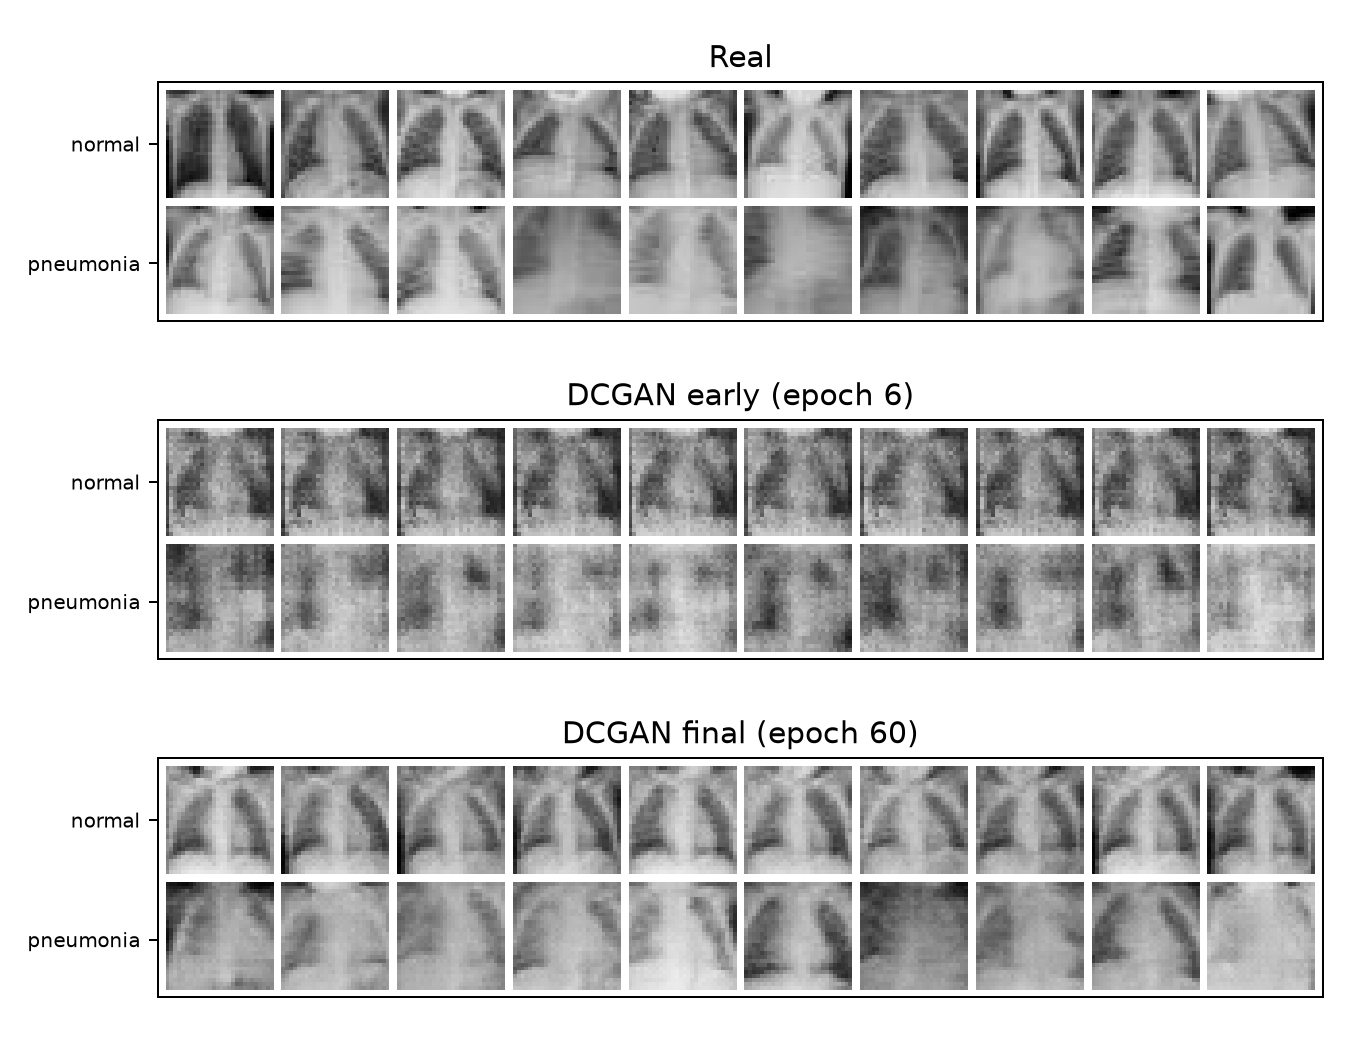
\includegraphics[width=0.9\linewidth]{figures/pneumonia_real_vs_synthetic.png}
\caption{PneumoniaMNIST: real training images (top), early generator after 6 epochs (middle), final generator after 60
epochs (bottom); one row per class.}
\label{fig:pneu_samples}
\end{figure}

\begin{table}[htbp]
\centering
\caption{PneumoniaMNIST, real test set (624 images), mean $\pm$ std over 3 seeds, 15 classifier epochs. $p$: Welch's
$t$-test on per-seed macro F1 vs.\ real only. Normal recall = recall of the minority class \emph{normal}.
Source: \texttt{results/pneumoniamnist/}.}
\label{tab:pneu}
\resizebox{\linewidth}{!}{%
\begin{tabular}{lcccccc}
\toprule
Setting & Accuracy & Macro F1 & AUC & Normal recall & $\Delta$F1 & $p$ \\
\midrule
Real only (0\%)     & \textbf{0.880 $\pm$ 0.017} & \textbf{0.861 $\pm$ 0.021} & 0.973 $\pm$ 0.006 & \textbf{0.691} & --       & --    \\
Real + flip/shift   & 0.808 $\pm$ 0.069 & 0.755 $\pm$ 0.104 & 0.972 $\pm$ 0.010 & 0.489 & $-$0.106 & 0.215 \\
\midrule
+50\% GAN (final)   & 0.860 $\pm$ 0.026 & 0.834 $\pm$ 0.035 & 0.973 $\pm$ 0.005 & 0.634 & $-$0.027 & 0.334 \\
+100\% GAN (final)  & 0.873 $\pm$ 0.006 & 0.853 $\pm$ 0.008 & 0.975 $\pm$ 0.002 & 0.668 & $-$0.008 & 0.573 \\
+200\% GAN (final)  & 0.875 $\pm$ 0.003 & 0.855 $\pm$ 0.004 & \textbf{0.976 $\pm$ 0.002} & 0.671 & $-$0.006 & 0.652 \\
+100\% GAN (early)  & 0.868 $\pm$ 0.005 & 0.845 $\pm$ 0.006 & 0.973 $\pm$ 0.001 & 0.651 & $-$0.016 & 0.317 \\
GAN class balancing & 0.863 $\pm$ 0.015 & 0.838 $\pm$ 0.019 & 0.973 $\pm$ 0.002 & 0.635 & $-$0.023 & 0.240 \\
\bottomrule
\end{tabular}}
\end{table}

\begin{figure}[htbp]
\centering
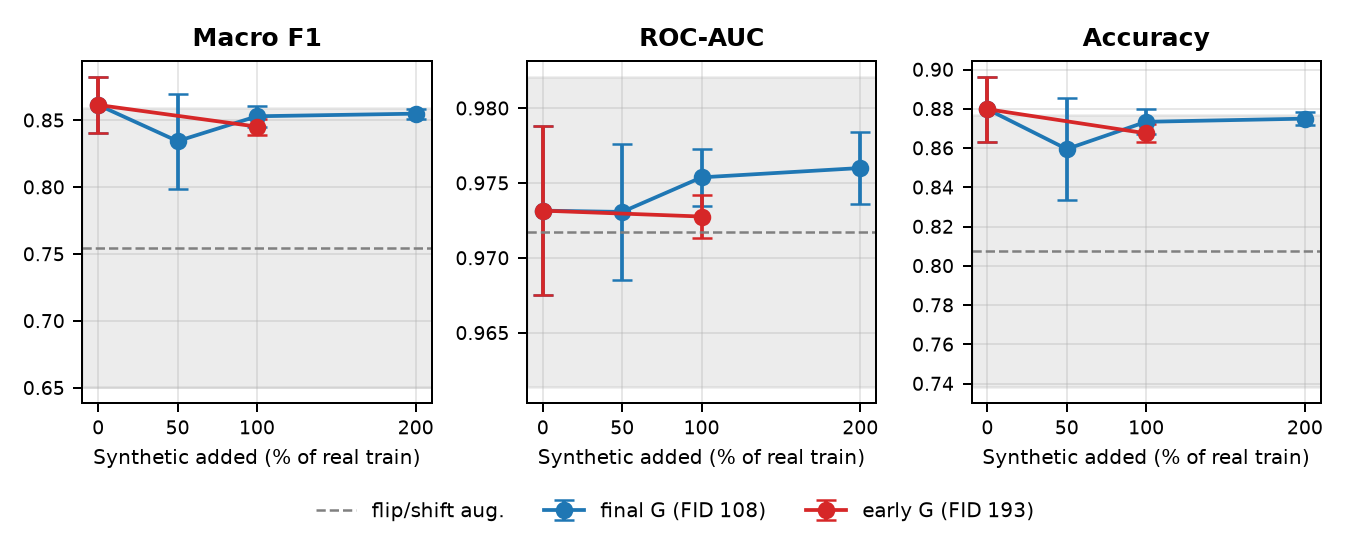
\includegraphics[width=\linewidth]{figures/pneumonia_metrics_vs_ratio.png}
\caption{PneumoniaMNIST: metrics against the amount of synthetic data. Note how the error bars shrink as more synthetic
images are added, while the means stay at the real-only level.}
\label{fig:pneu_ratio}
\end{figure}

\noindent Table~\ref{tab:pneu} and Figure~\ref{fig:pneu_ratio} show the same overall answer as on BreastMNIST, with two
instructive differences:
\begin{enumerate}
  \item \textbf{Again, no F1 gain.} No GAN setting beats the real-only baseline (F1 0.861); differences range from
        $-0.027$ to $-0.006$ and none is significant (all $p>0.2$). The real-only baseline (accuracy 0.880, AUC 0.973)
        is above the MedMNIST v2 ResNet-18 reference (0.854 / 0.944).
  \item \textbf{Synthetic data stabilises training here.} The seed-to-seed standard deviation of F1 falls from 0.021
        (real only) to 0.008 (+100\%) and 0.004 (+200\%), and the +200\% setting has the highest AUC (0.976). With a
        larger real set, the GAN is a better model of the data and its images act as a mild regulariser.
  \item \textbf{Quality still matters.} At +100\%, the final generator beats the early one on every metric (F1 0.853
        vs.\ 0.845, AUC 0.975 vs.\ 0.973, normal recall 0.668 vs.\ 0.651).
  \item \textbf{Classical augmentation hurts on chest X-rays.} Horizontal flipping drops F1 to 0.755 and normal recall to
        0.489. A mirrored chest X-ray puts the heart on the wrong side -- an anatomically impossible image -- whereas a
        mirrored breast ultrasound is still realistic. Augmentation must respect the anatomy of the modality.
  \item \textbf{All models under-detect the normal class.} Pneumonia recall is above 0.99 in every setting, but normal
        recall is only 0.49--0.69, so most errors are normal patients predicted as pneumonia. Neither proportional
        augmentation nor GAN class balancing (normal recall 0.635) fixed this.
\end{enumerate}

% -------------------------------------------------------------------------------------
\FloatBarrier
\section{Discussion}
\textbf{Answer to the research question.} In our setting, adding DCGAN-generated images did \emph{not} improve a CNN
classifier on real test images, on either dataset, at any amount (50--200\%) or quality (FID 86 vs.\ 135). This
differs from the improvement reported by Frid-Adar et al.~\cite{fridadar2018gan}, and we see four reasons in our results.

\begin{enumerate}
  \item \textbf{A GAN cannot add information it never saw.} The generator is trained on the same 546 (or 4{,}708)
        images as the classifier. Our memorisation check shows that it does not copy them, but the samples are
        variations of the same visual content -- with limited diversity (near-duplicate samples, Figure~\ref{fig:nn}).
        New \emph{information} about rare cases (e.g.\ unusual malignant lesions) can only come from new real data.
  \item \textbf{The quality gap acts like label noise.} With FID 86 against a real-vs-real floor of 59, part of the
        synthetic images are not clearly typical of their class. When such images make up a third to two thirds of the
        training set, the classifier partly learns GAN artefacts and ambiguous class boundaries; on BreastMNIST this
        shows up as a lower and less stable F1 at 50--100\%.
  \item \textbf{Quantity helps ranking more than decisions.} At 200\%, AUC is the best of all settings on both datasets
        (0.922 and 0.976), so synthetic images seem to regularise the learned features; but the decision threshold
        shifts towards the majority class (malignant recall 0.638). A threshold tuned on validation data might
        turn this AUC gain into an F1 gain -- a cheap follow-up experiment.
  \item \textbf{Better images help, but not enough.} The final generator beats the early one in AUC at every BreastMNIST
        ratio and on every PneumoniaMNIST metric, so quality clearly matters; the trend suggests that a stronger
        generator (StyleGAN2-ADA, diffusion) is a prerequisite for gains, not an option.
\end{enumerate}

\textbf{Dataset size changes the role of synthetic data.} With 546 images, synthetic data mainly added variance; with
4{,}708 images it reduced variance (std of F1 from 0.021 to 0.004). A GAN trained on more data is a better model of
that data, and its samples then behave like a smooth regulariser rather than noise.

\textbf{Classical augmentation must match the modality.} Simple flips and shifts were the best method for breast
ultrasound (F1 +0.022, malignant recall +0.076) but the worst for chest X-rays (F1 $-0.106$), because a mirrored chest is
anatomically wrong. Domain knowledge matters more than the sophistication of the augmentation method.

\textbf{Why multiple seeds were essential.} With a single seed we could have reported almost any conclusion: individual
BreastMNIST runs of +50\% GAN range from accuracy 0.686 to 0.891. Only the mean over seeds, the standard deviation and the
$t$-test reveal that none of the differences is reliable -- a methodological point that much of the GAN-augmentation
literature does not address.

\textbf{Practical recommendation.} For a small medical dataset, first use modality-appropriate classical augmentation and
report results over several seeds; consider GAN augmentation only with a generator whose FID is close to the real-vs-real
floor, check it for memorisation, and evaluate it against the classical baseline as done here.

\section{Limitations and Future Work}
\begin{itemize}
  \item \textbf{Resolution.} We used 28$\times$28 images to fit a CPU budget; fine lesion details are lost. MedMNIST+ offers
        64--224\,px versions on which both the GAN and the classifier could behave differently.
  \item \textbf{Generator family.} DCGAN is a 2016 architecture. StyleGAN2-ADA or diffusion models produce markedly better
        samples on small datasets and may change the conclusion.
  \item \textbf{Metric mismatch.} FID relies on ImageNet features that are poorly suited to grayscale ultrasound; a
        medical-domain feature extractor would give a more meaningful quality score.
  \item \textbf{Statistics.} Five (three) seeds give a rough estimate of variance; the BreastMNIST test set has only
        42 malignant images, so a single changed prediction moves recall by 2.4 points.
  \item \textbf{Single classifier.} We used one small CNN; a larger or pretrained model may benefit differently from
        synthetic data.
  \item \textbf{No clinical validation.} Synthetic images were not reviewed by radiologists; the system is a research
        prototype, not a diagnostic tool.
\end{itemize}

\section{Conclusion}
We built a complete, reproducible pipeline to test whether GAN-generated images help a classifier trained on a small
medical dataset. A class-conditional DCGAN with DiffAugment-style translation learned realistic-looking breast ultrasound
and chest X-ray images without memorising its training data, and a better generator (lower FID) consistently gave better
classifiers than a worse one. Nevertheless, adding 50--200\% synthetic images did not improve macro F1 on real test
images for either dataset, and no difference was statistically significant over 5 (3) seeds. Synthetic data raised AUC
slightly at 200\% and, on the larger dataset, made training much more stable, while simple flip/shift augmentation was the
best method for ultrasound but harmful for chest X-rays. The answer to ``does synthetic data help?'' is therefore:
\emph{not by itself with a DCGAN at this scale -- quality, dataset size and the choice of baseline decide}.
Future work: higher resolution (MedMNIST+), stronger generators (StyleGAN2-ADA, diffusion), threshold tuning, and
filtering synthetic images by classifier confidence before adding them.

\section*{Code Availability and Demo}
Code, results and instructions: \url{https://github.com/Bhagwati23/GAN-medicalAugmentation}. The package \texttt{ganaug}
contains one module per stage (data, DCGAN, GAN training, augmentation, classifier, FID, experiments, report figures);
\texttt{tests/} checks shapes, determinism and that synthetic images never reach the validation or test sets; a GitHub
Actions workflow runs these tests on every pull request. \texttt{app.py} is a Gradio web app that generates synthetic images
for a chosen class and generator checkpoint, classifies an uploaded or real test image with both the real-only and the
GAN-augmented classifier side by side, and shows the result tables.

\section*{Individual Contributions}
\begin{itemize}
  \item \textbf{Arjun Kadam} (su-24022@sitare.org): synthetic-data augmentation pipeline (issue \#5), integration, testing,
        CI and reproducibility (\#8), demo application, project report (\#9).
  \item \textbf{Bhagwati} (su-24032@sitare.org): conditional DCGAN architecture (\#3), GAN training, checkpoints and samples (\#4), independent re-run of GAN training (reproducibility check);
        repository set-up, issue planning, team workflow, and PR review and merge coordination.
  \item \textbf{Maneesh Sakhwar} (su-24068@sitare.org): dataset selection, loading, exploration notebook and data-leakage tests (\#1); FID/KID evaluation
        and memorisation check (\#6).
  \item \textbf{Anand Singh} (su-24014@sitare.org): CNN baseline (\#2); experiment runs, comparison tables and figures (\#7).
\end{itemize}

.
% Every number comes from results/ in the repository (see the table/figure captions).
% =====================================================================================

\begin{abstract}
Medical image datasets are often small and class-imbalanced, which limits how well deep classifiers can be trained.
We study whether images generated by a Generative Adversarial Network (GAN) can make up for this.
We train a class-conditional DCGAN on the training split of BreastMNIST (546 breast ultrasound images, 27\% malignant)
and add 0, 50, 100 or 200\% synthetic images to the training set of a CNN classifier, which is always evaluated on the
same held-out set of \emph{real} test images. To separate the effect of the \emph{amount} of synthetic data from its
\emph{quality}, we repeat every experiment with an early generator checkpoint (FID 134.9) and the fully trained
generator (FID 86.4; the real-vs-real reference is 59.1), compare against classical flip/shift augmentation and
against GAN-based class balancing, run five random seeds per setting, and test significance with Welch's $t$-test.
The generator learns realistic images without memorising the training set, and the better generator consistently beats
the worse one. Yet no amount of synthetic data improves macro F1 over real-only training (0.812; changes from $-0.054$ to
$+0.006$, none significant), while simple flip/shift augmentation gives the best F1 (0.834). Adding 200\% synthetic images
yields the highest AUC (0.922 vs.\ 0.911) but lowers malignant recall.
A second, nine times larger dataset (PneumoniaMNIST) is used to check whether the conclusion depends on dataset size.
All code, results and an interactive demo are available at \url{https://github.com/Bhagwati23/GAN-medicalAugmentation}.

\vspace{0.5cm}
\noindent
{\em Key Words}: Generative Adversarial Networks, DCGAN, Data Augmentation, Medical Image Classification,
Synthetic Data, MedMNIST, FID.
\end{abstract}
\hrulefill

% -------------------------------------------------------------------------------------
\section{Introduction}
Deep convolutional networks need many labelled examples, but labelled medical images are expensive: they require
expert annotation, are protected by privacy rules, and positive (disease) cases are rare. The usual remedy is
\emph{data augmentation}: creating new training examples from existing ones. Classical augmentation applies simple
geometric or photometric transforms (flips, shifts, rotations, contrast changes)~\cite{shorten2019survey}. Generative
Adversarial Networks (GANs)~\cite{goodfellow2014gan} offer a more ambitious option: learn the distribution of the
training images and sample entirely new ones. Frid-Adar et al.~\cite{fridadar2018gan} reported that GAN-generated
liver-lesion images raised CNN sensitivity and specificity, which made GAN augmentation popular in medical
imaging~\cite{yi2019ganmedical}.

However, a GAN trained on a small dataset only sees the same few hundred images as the classifier. It is therefore not
obvious that its samples add \emph{new information}; they may only add noise, or copies of the training images.
This project asks a precise question:

\begin{quote}
\emph{When a classifier is trained on a small medical dataset, does adding GAN-generated images improve its performance
on real, unseen images -- and how does the gain depend on the amount and on the quality of the synthetic data?}
\end{quote}

\noindent\textbf{Contributions.}
\begin{itemize}
  \item A reproducible pipeline (MedMNIST v2 data, class-conditional DCGAN, augmentation at 0/\allowbreak 50/\allowbreak 100/\allowbreak 200\%, CNN
        classifier, FID/KID evaluation) with strict separation of training, validation and test data.
  \item A two-axis study: \emph{quantity} (four synthetic ratios) $\times$ \emph{quality} (early vs.\ final generator,
        measured by FID and KID), plus two reference points: classical flip/shift augmentation and GAN class balancing.
  \item Statistical care: five seeds per setting, mean $\pm$ standard deviation, Welch's $t$-test against the real-only baseline.
  \item Checks that the generator does not simply memorise the training set (nearest-neighbour distances and latent
        interpolation).
  \item A replication on a second, larger dataset (PneumoniaMNIST) and an interactive web demo.
\end{itemize}

\begin{keybox}{Key findings at a glance}
\begin{itemize}
  \item \textbf{No F1 gain from GAN images} on either dataset at 50, 100 or 200\% synthetic data (BreastMNIST real-only
        F1 0.812 vs.\ 0.758--0.819 with GAN data; none significant, all $p>0.2$).
  \item \textbf{Quality matters:} the better generator (FID 86) beats the early one (FID 135) in AUC at every ratio.
  \item \textbf{200\% synthetic gives the best AUC} on both datasets (0.922 and 0.976) and, on the larger dataset,
        cuts seed-to-seed variance five-fold.
  \item \textbf{No memorisation:} no generated image is closer to a training image than typical unseen real images.
  \item \textbf{Classical augmentation depends on anatomy:} best for breast ultrasound (F1 0.834), harmful for chest
        X-rays (F1 0.755) because mirrored chests are anatomically wrong.
\end{itemize}
\end{keybox}

% -------------------------------------------------------------------------------------
\section{Related Work}
\textbf{GANs and DCGAN.} A GAN~\cite{goodfellow2014gan} trains a generator $G$ to map random noise $z$ to images and a
discriminator $D$ to tell real from generated images; the two are trained against each other. DCGAN~\cite{radford2016dcgan}
gave architectural rules that make this training stable for images: strided (transposed) convolutions instead of pooling,
batch normalisation, ReLU in $G$, LeakyReLU in $D$, Adam with learning rate $2\times10^{-4}$ and $\beta_1=0.5$.
Conditional GANs~\cite{mirza2014cgan} feed the class label to both networks so that images of a chosen class can be requested.

\textbf{GANs with little data.} With few training images the discriminator quickly memorises them and stops giving
useful gradients. DiffAugment~\cite{zhao2020diffaugment} applies the same random, differentiable augmentation to real and
generated images before the discriminator, which strongly improves GANs trained on a few hundred images.

\textbf{GAN augmentation in medical imaging.} Frid-Adar et al.~\cite{fridadar2018gan} generated liver-lesion CT patches
with DCGAN and improved classification from 78.6\% to 85.7\% sensitivity. Reviews~\cite{yi2019ganmedical} report
mixed results in later work, often without multiple seeds or a comparison with classical augmentation -- gaps this
project addresses.

\textbf{Evaluating generated images.} The Fr\'echet Inception Distance (FID)~\cite{heusel2017fid} compares Inception-v3
feature statistics of real and generated images; the Kernel Inception Distance (KID)~\cite{binkowski2018kid} is an
unbiased alternative better suited to small samples. Ravuri and Vinyals~\cite{ravuri2019cas} showed that such scores do not
fully predict how useful samples are for training a classifier -- which is exactly what our classifier experiments measure.

\textbf{MedMNIST.} MedMNIST v2~\cite{yang2023medmnist} provides standardised, pre-split 28$\times$28 biomedical datasets with
benchmark results, which makes our numbers comparable and reproducible.

% -------------------------------------------------------------------------------------
\section{Datasets}
We use two binary datasets from MedMNIST v2~\cite{yang2023medmnist} at their default 28$\times$28 grayscale resolution and
keep the \emph{official} train/validation/test splits (Table~\ref{tab:data}, Fig.~\ref{fig:data}).

\textbf{BreastMNIST} (main dataset) is derived from a breast ultrasound dataset~\cite{aldhabyani2020busi}; the label is
\emph{malignant} (class 0) or \emph{normal/benign} (class 1). With only 546 training images and 27\% malignant cases it is
exactly the small, imbalanced setting in which synthetic data is supposed to help.

\textbf{PneumoniaMNIST} (second dataset) is derived from paediatric chest X-rays~\cite{kermany2018pneumonia}: \emph{normal}
(class 0) vs.\ \emph{pneumonia} (class 1), with 4{,}708 training images (about nine times more). It tells us whether a
conclusion drawn on BreastMNIST changes when real data is more plentiful.

\begin{table}[htbp]
\centering
\caption{Official MedMNIST v2 splits (images per class). Source: \texttt{results/dataset\_stats.json}.}
\label{tab:data}
\begin{tabular}{llrrr}
\toprule
Dataset & Class & Train & Val & Test \\
\midrule
BreastMNIST    & malignant      & 147   & 21  & 42  \\
               & normal/benign  & 399   & 57  & 114 \\
               & \emph{total}   & 546   & 78  & 156 \\
\midrule
PneumoniaMNIST & normal         & 1{,}214 & 135 & 234 \\
               & pneumonia      & 3{,}494 & 389 & 390 \\
               & \emph{total}   & 4{,}708 & 524 & 624 \\
\bottomrule
\end{tabular}
\end{table}

\begin{figure}[htbp]
\centering
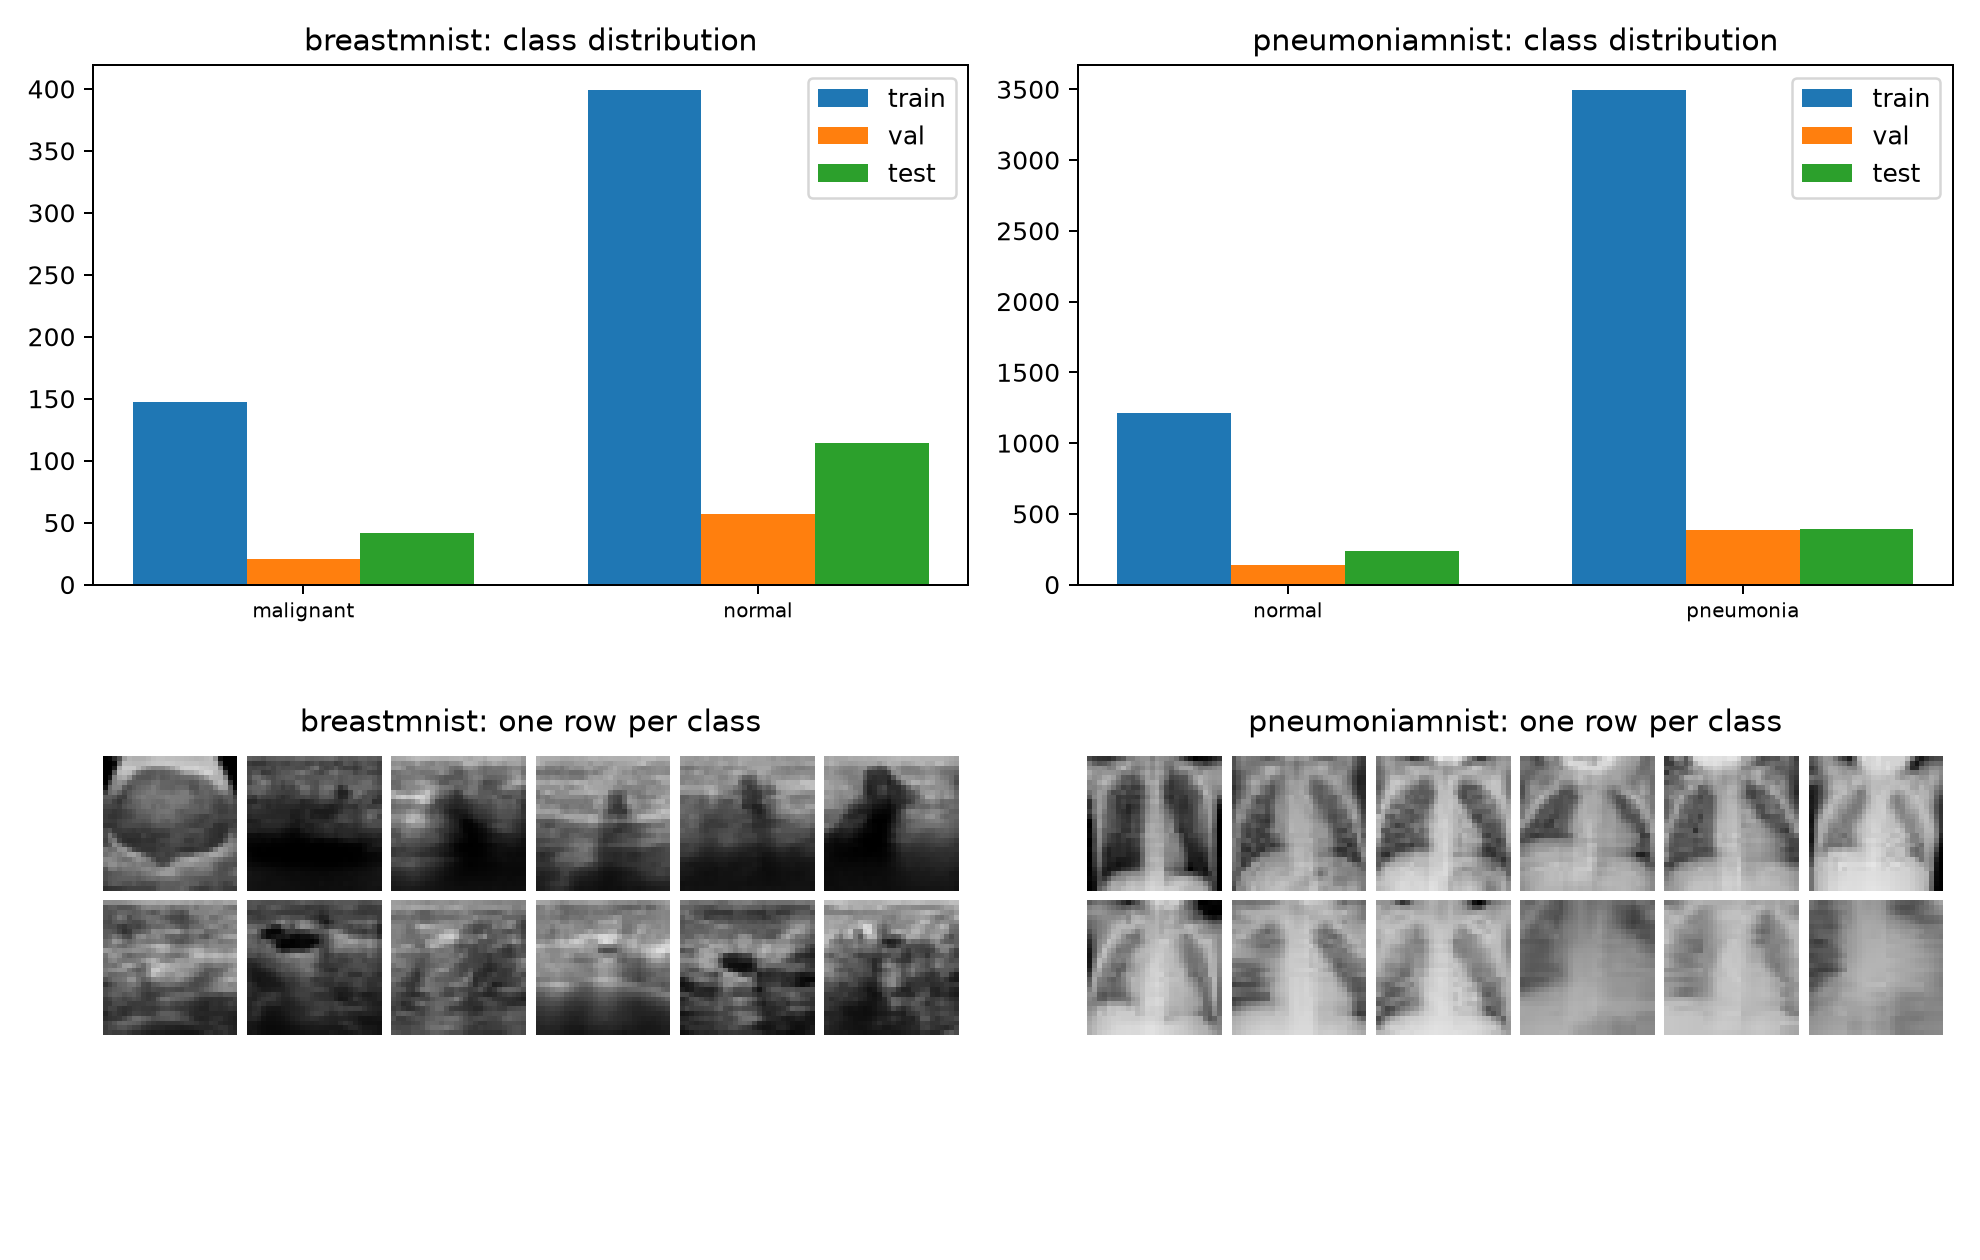
\includegraphics[width=\linewidth]{figures/dataset_overview.png}
\caption{Class distribution per split (top) and training images, one row per class (bottom). Both datasets are imbalanced
(minority class: malignant in BreastMNIST, normal in PneumoniaMNIST).}
\label{fig:data}
\end{figure}

\textbf{Preprocessing and leakage control.} Pixel values are scaled from $[0,255]$ to $[-1,1]$, the output range of the
generator's $\tanh$. The GAN is trained \emph{only} on the training split. Synthetic images are added \emph{only} to the
training split. Validation (used to choose the best epoch) and test (used once, for the final numbers) contain only real
images and are identical in every experiment. These rules are enforced in code and checked by unit tests.

% -------------------------------------------------------------------------------------
\section{Method}

\subsection{Pipeline}
\begin{enumerate}
  \item Train a class-conditional DCGAN on the real training images; save an \emph{early} checkpoint (after 10\% of
        training) and the \emph{final} one.
  \item Score both generators with FID and KID against the real training images, and check for memorisation.
  \item For each setting (Section~\ref{sec:settings}), build a training set of real images plus a controlled number of
        synthetic images, train the CNN classifier with five seeds, and evaluate on the real test set.
  \item Compare every setting with the real-only baseline (mean, standard deviation, Welch's $t$-test).
\end{enumerate}

\subsection{Class-conditional DCGAN}
Table~\ref{tab:gan} lists the architecture. The generator concatenates a 100-dimensional Gaussian noise vector $z$ with a
learned 50-dimensional embedding of the class label $y$, projects it to a $256\times7\times7$ tensor and upsamples it with
two stride-2 transposed convolutions to $28\times28$. The discriminator receives the image together with a learned
$28\times28$ ``label map'' as a second channel, so it judges whether the image is realistic \emph{for that class}.
Following DCGAN~\cite{radford2016dcgan}, weights are initialised from $\mathcal{N}(0,0.02)$, $G$ uses BatchNorm + ReLU and
$D$ uses LeakyReLU(0.2), no pooling layers.

\begin{table}[htbp]
\centering
\caption{Conditional DCGAN architecture (\texttt{ganaug/dcgan.py}). ConvT = transposed convolution, k = kernel, s = stride.}
\label{tab:gan}
\small
\begin{tabular}{ll}
\toprule
\multicolumn{2}{l}{\textbf{Generator} (2.56\,M parameters)} \\
Input & $z\in\mathbb{R}^{100}$ $\oplus$ Embedding$(y)\in\mathbb{R}^{50}$ \\
Linear + BN + ReLU & $150 \rightarrow 256\times7\times7$ \\
ConvT k4 s2 + BN + ReLU & $\rightarrow 128\times14\times14$ \\
ConvT k4 s2 + BN + ReLU & $\rightarrow 64\times28\times28$ \\
Conv k3 s1 + $\tanh$ & $\rightarrow 1\times28\times28$, values in $[-1,1]$ \\
\midrule
\multicolumn{2}{l}{\textbf{Discriminator} (0.43\,M parameters)} \\
Input & image $\oplus$ label map $\rightarrow 2\times28\times28$ \\
Conv k4 s2 + LeakyReLU & $\rightarrow 64\times14\times14$ \\
Conv k4 s2 + BN + LeakyReLU & $\rightarrow 128\times7\times7$ \\
Conv k3 s2 + BN + LeakyReLU & $\rightarrow 256\times4\times4$ \\
Dropout(0.3) + Linear & $\rightarrow$ 1 logit (real/fake) \\
\bottomrule
\end{tabular}
\end{table}

\textbf{Training objective.} With $\sigma$ the sigmoid and $\tilde{x}=T(x)$ a random translation (below), $D$ minimises
\begin{equation}
\mathcal{L}_D = -\,\mathbb{E}_{x,y}\big[\,0.9\log\sigma(D(\tilde{x},y))\big] - \mathbb{E}_{z,y}\big[\log\big(1-\sigma(D(\widetilde{G(z,y)},y))\big)\big],
\end{equation}
and $G$ minimises the non-saturating loss $\mathcal{L}_G = -\,\mathbb{E}_{z,y}\big[\log\sigma(D(\widetilde{G(z,y)},y))\big]$.
Two additions help with only 546 training images:
(i) \emph{one-sided label smoothing}: the target for real images is 0.9 instead of 1, so $D$ does not become over-confident;
(ii) \emph{DiffAugment-style translation}~\cite{zhao2020diffaugment}: every real and generated image is shifted by a random
$-2\ldots2$ pixels (edge-replicate padding) before it is shown to $D$, which keeps $D$ from memorising the training images.
Both networks use Adam ($2\times10^{-4}$, $\beta=(0.5,0.999)$), batch size 64.

\subsection{Augmentation protocol}
\label{sec:aug}
For a ratio $r\in\{0, 0.5, 1, 2\}$ we add $\mathrm{round}(r\cdot n_c)$ synthetic images of each class $c$, where $n_c$ is
the number of real training images of class $c$. This keeps the real class ratio (for BreastMNIST: $+50\%$ = 274,
$+100\%$ = 546, $+200\%$ = 1{,}092 synthetic images). For each generator we sample one fixed pool of synthetic images
(fixed seed) and every ratio takes the first $k$ images of each class, so the sets are \emph{nested}
($50\% \subset 100\% \subset 200\%$): differences between ratios come from the amount of data, not from a luckier draw.
In the \emph{class-balancing} setting we instead add only minority-class images until both classes have the same size
(BreastMNIST: 252 synthetic malignant images, giving 399 vs.\ 399).

\subsection{Classifier}
All settings use the same CNN (\texttt{ganaug/cnn.py}, 0.29\,M parameters): three blocks of
[Conv3$\times$3--BN--ReLU]$\times$2 + MaxPool with 32, 64 and 128 channels ($28\to14\to7\to3$), global average pooling,
dropout 0.3 and a linear layer. It is trained with cross-entropy, AdamW (learning rate $10^{-3}$, weight decay $10^{-4}$),
a cosine learning-rate schedule and batch size 64. After each epoch we compute the validation ROC-AUC and keep the weights
with the best value (model selection on validation, never on test). The model is deliberately small: the dataset is tiny
and all experiments ran on a CPU. Our real-only baseline (Section~\ref{sec:results}) is in line with the ResNet-18 results
reported by MedMNIST v2~\cite{yang2023medmnist} (BreastMNIST, 28$\times$28: accuracy 0.863, AUC 0.901).

\subsection{Evaluation}
\textbf{Classifier metrics} (real test set): accuracy; \emph{macro} precision, recall and F1 (each class weighted
equally, so missing the minority class is penalised; macro recall equals balanced accuracy); ROC-AUC (threshold-free
ranking quality); and confusion matrices. Macro F1 is our main metric because accuracy can look good on imbalanced data
by mostly predicting the majority class.

\textbf{Image quality.} FID and KID are computed with \texttt{torch-fidelity} between the real training images and the
same number of generated images with the same class ratio (images converted to 3-channel uint8 and resized to
299$\times$299 for Inception-v3). Because 28$\times$28 grayscale ultrasound images are very different from ImageNet photos,
absolute FID values are not comparable to natural-image papers; we therefore also report FID between the real training and
real test images as a \emph{reference floor}.

\textbf{Memorisation check.} For every generated image we find the closest real training image (pixel $L_2$ distance) and
compare these distances with the same distances for real \emph{test} images, which are realistic but unseen. A generator
that copies training images would produce many samples closer to the training set than almost any real test image; we
report the fraction of generated images closer than the 5th percentile of the test distances (about 0.05 is expected if
there is no copying).

\textbf{Statistics.} Each setting is trained with seeds 0--4 (BreastMNIST) or 0--2 (PneumoniaMNIST); we report mean
$\pm$ standard deviation and a two-sided Welch's $t$-test of the per-seed macro F1 against the real-only baseline.

% -------------------------------------------------------------------------------------
\section{Experimental Setup}
\label{sec:settings}
\begin{table}[htbp]
\centering
\caption{Experiment settings. Only the training set changes; the CNN, its hyper-parameters, and the validation and test
sets are identical everywhere.}
\label{tab:settings}
\small
\begin{tabular}{lp{5.2cm}}
\toprule
Setting & Training data \\
\midrule
Real only (0\%) & real training images (baseline) \\
Real + flip/shift & real images, random horizontal flip and $\pm2$\,px shift on the fly \\
+50/100/200\% GAN (final) & real + synthetic from the final generator \\
+50/100/200\% GAN (early) & real + synthetic from the early generator \\
GAN class balancing & real + synthetic minority-class images until classes are equal \\
\bottomrule
\end{tabular}
\end{table}

\begin{table}[htbp]
\centering
\caption{Training configuration.}
\label{tab:hparams}
\small
\begin{tabular}{lll}
\toprule
 & BreastMNIST & PneumoniaMNIST \\
\midrule
GAN epochs (updates)       & 300 (2{,}400) & 60 (4{,}380) \\
Early checkpoint           & epoch 30      & epoch 6 \\
Classifier epochs          & 40            & 15 \\
Seeds per setting          & 5             & 3 \\
Settings run               & all 9         & 7 (no early 50/200\%) \\
FID sample size            & 546           & 2{,}000 (random subset) \\
\bottomrule
\end{tabular}
\end{table}

All experiments ran on a laptop CPU with PyTorch. Table~\ref{tab:settings} lists the settings and Table~\ref{tab:hparams}
the configuration. Because PneumoniaMNIST is nine times larger, we used fewer classifier epochs, seeds and settings for it.
Everything is reproduced by \texttt{bash run\_all.sh}.

% -------------------------------------------------------------------------------------
\FloatBarrier
\section{Results}
\label{sec:results}

\subsection{Quality of the synthetic images}
\textbf{Training dynamics.} Figure~\ref{fig:losses} shows that GAN training on BreastMNIST stayed balanced for all 300
epochs: the discriminator loss stays close to $2\ln 2\approx1.39$ (the value when $D$ cannot separate real from fake), and
at the end $D$ assigns on average 0.46 to real and 0.44 to generated images. There is no sign of mode collapse (where
$D(G(z))$ would drop to 0 and all samples would look alike) or of $D$ winning outright.

\textbf{Reproducibility of GAN training.} The GAN training was run twice, independently, on two different laptops with
the same code, configuration and seed: run~1 produced the generators used for every experiment in this report, and run~2
(by Bhagwati, committed as the training log in \texttt{results/}) checks that training can be repeated. Averaged over the
last 10\% of epochs, the two runs agree closely: BreastMNIST discriminator loss 1.371 vs.\ 1.377, $D(x)$ 0.459 vs.\ 0.456
and $D(G(z))$ 0.441 vs.\ 0.444; PneumoniaMNIST discriminator loss 1.376 vs.\ 1.377, $D(x)$ 0.455 vs.\ 0.456. Bit-exact
equality is not expected, because CPU floating-point operations are not deterministic across machines and library
versions, but the training reaches the same balanced state.

\begin{figure}[htbp]
\centering
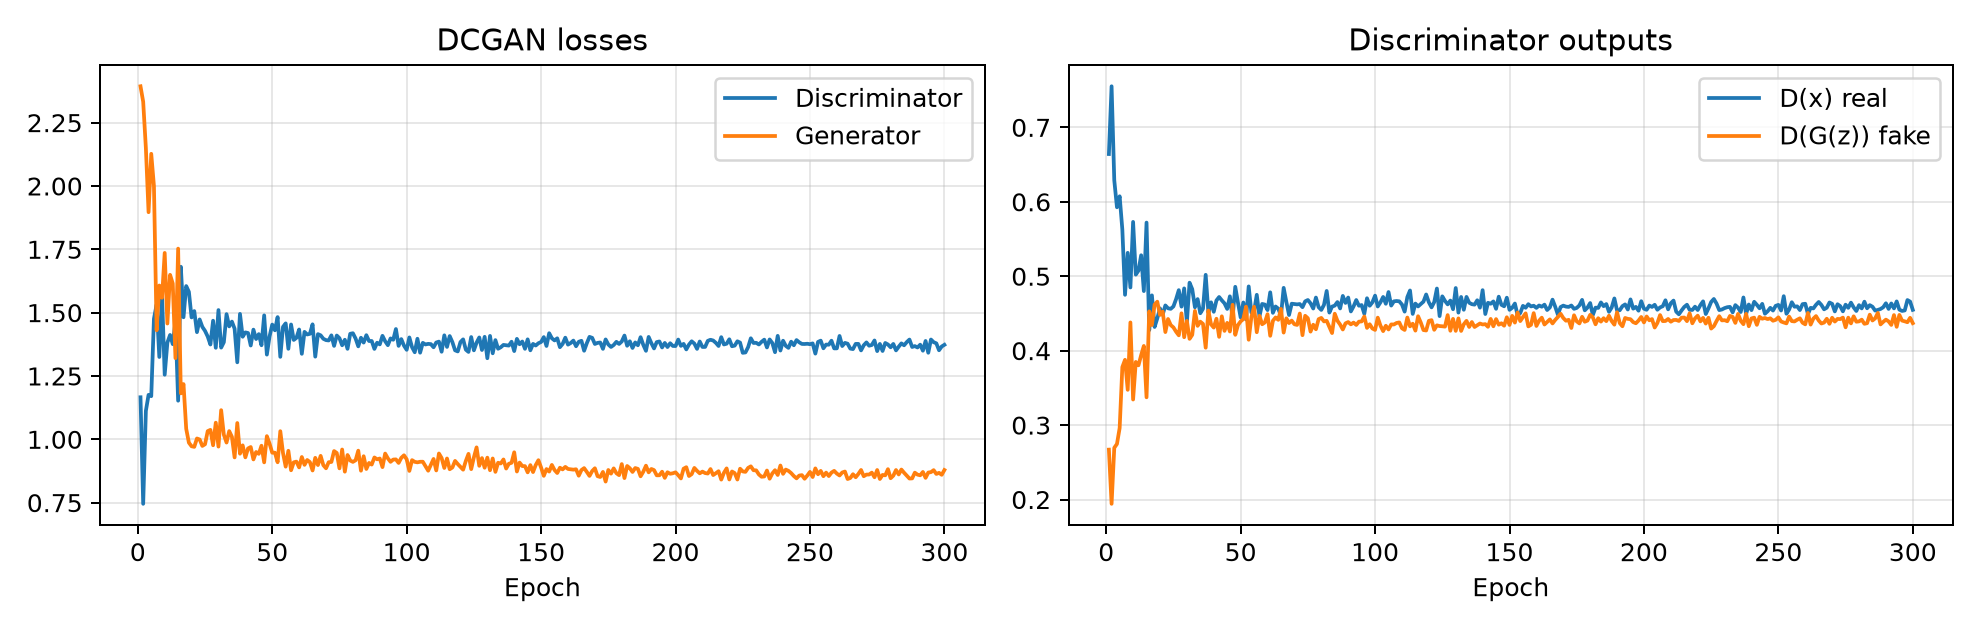
\includegraphics[width=\linewidth]{figures/breast_gan_losses.png}
\caption{DCGAN training on BreastMNIST. Left: losses. Right: mean discriminator output for real ($D(x)$) and generated
($D(G(z))$) images; both stay close to 0.5, i.e.\ a balanced adversarial game. Source: \texttt{results/breastmnist/report\_run/gan\_losses.csv} (run~1).}
\label{fig:losses}
\end{figure}

\textbf{Visual quality.} Figure~\ref{fig:samples} compares real images with samples from both generators. After 30 epochs
the generator only reproduces the global layout (bright tissue at the top, dark region at the bottom) with heavy noise.
After 300 epochs the samples contain lesion-like dark regions and ultrasound speckle texture; synthetic \emph{malignant}
images tend to show larger, darker, irregular masses, matching the real malignant row. Small checkerboard artefacts from
the transposed convolutions remain.

\begin{figure}[htbp]
\centering
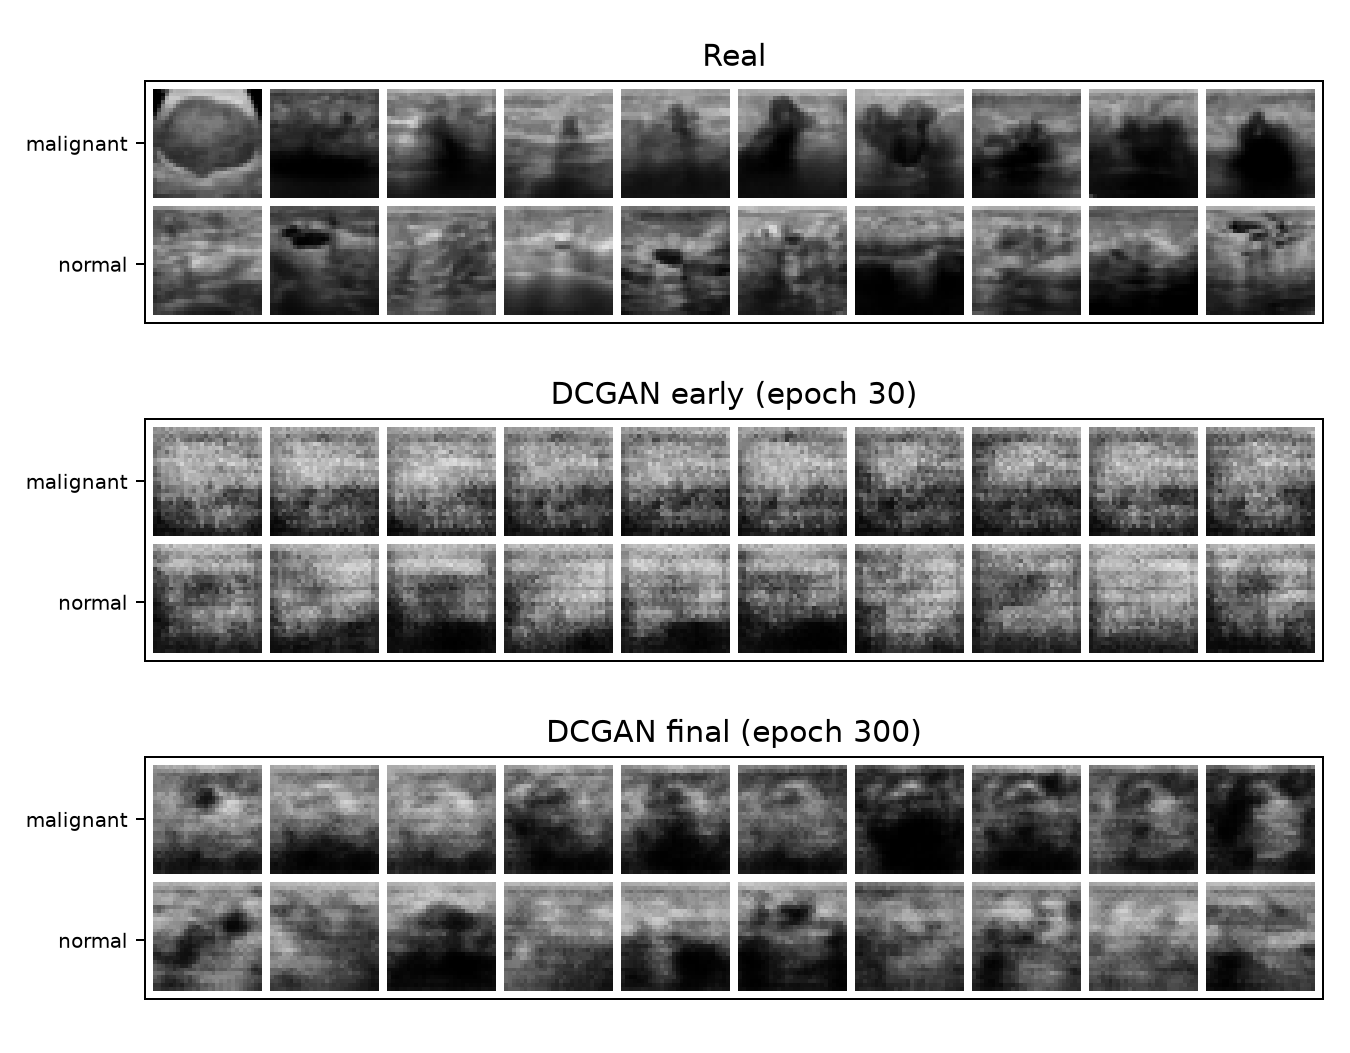
\includegraphics[width=0.9\linewidth]{figures/breast_real_vs_synthetic.png}
\caption{BreastMNIST: real training images (top), early generator after 30 epochs (middle) and final generator after 300
epochs (bottom); one row per class.}
\label{fig:samples}
\end{figure}

\textbf{FID and KID.} Table~\ref{tab:fid} quantifies the quality difference. The final generator reduces FID from 134.9 to
86.4 and KID by about half, but a gap to the real-vs-real reference (59.1) remains: the synthetic distribution is
clearly closer to the real one, yet not identical.

\begin{table}[htbp]
\centering
\caption{Image quality on BreastMNIST (546 images per set; lower is better). Source: \texttt{results/breastmnist/fid.json}.}
\label{tab:fid}
\small
\begin{tabular}{lrr}
\toprule
Compared with real training images & FID & KID \\
\midrule
Real test images (reference floor)   & 59.1  & 0.0004 \\
Early generator (epoch 30)           & 134.9 & 0.1220 \\
Final generator (epoch 300)          & 86.4  & 0.0670 \\
\bottomrule
\end{tabular}
\end{table}

\textbf{No memorisation.} The median distance from a generated image to its nearest training image is 6.33 (final) and
6.96 (early), larger than the 5.52 measured for real test images, and \emph{none} of the generated images is closer to a
training image than the closest 5\% of real test images (fraction 0.00 for both generators). Figure~\ref{fig:nn} shows
generated images next to their nearest training images: they share style but are not copies. The same figure also
shows a weakness: the first two generated images are almost identical to each other, a sign of \emph{limited diversity}
(partial mode collapse) -- the generator does not copy training images, but it also covers fewer distinct variations
than the real data. The latent interpolation in
Figure~\ref{fig:interp} changes smoothly from one image to another, which indicates that the generator learned a continuous
image distribution rather than a lookup table of training images.

\begin{figure}[htbp]
\centering
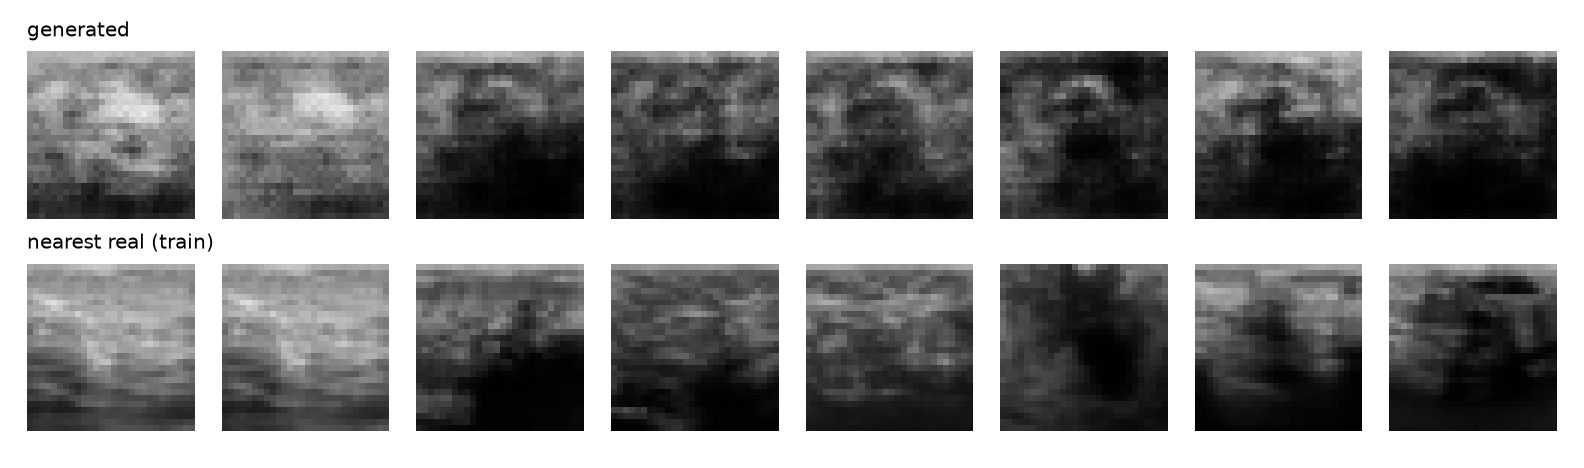
\includegraphics[width=\linewidth]{figures/breast_nearest_neighbours.png}
\caption{Top: images from the final generator. Bottom: the closest real training image to each (pixel $L_2$). Similar
style, different content: the generator does not copy training images. The first two samples are near-duplicates of
each other, showing limited sample diversity.}
\label{fig:nn}
\end{figure}

\begin{figure}[htbp]
\centering
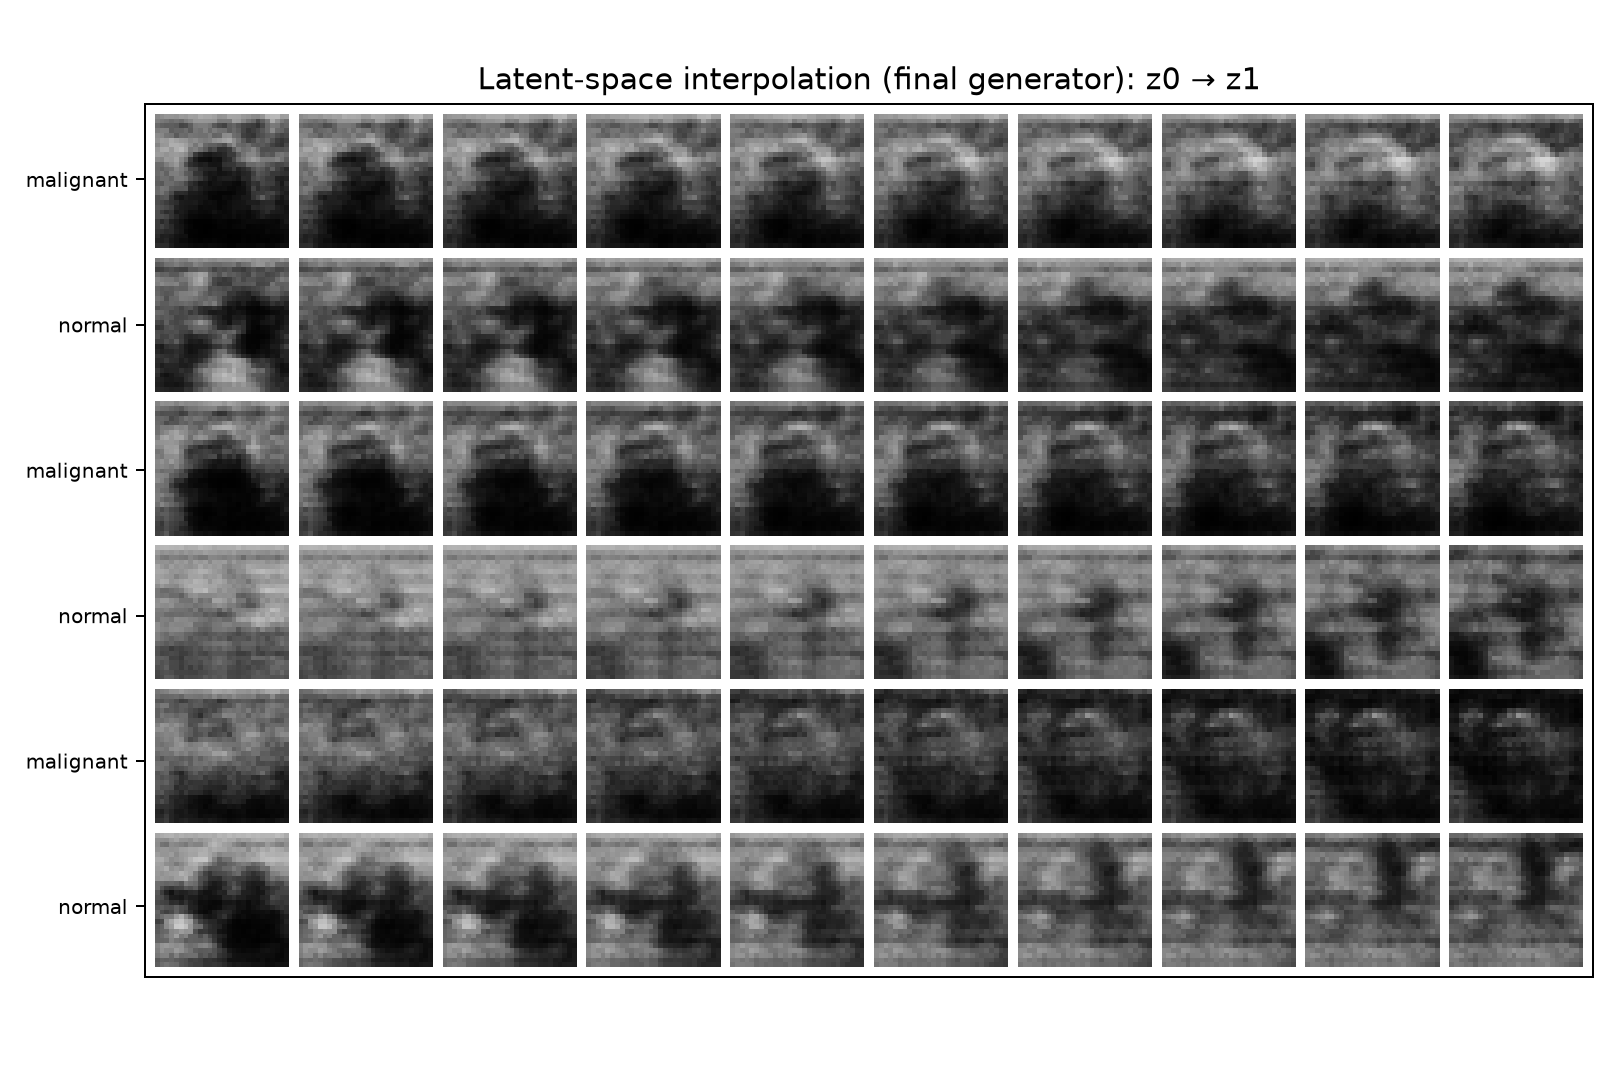
\includegraphics[width=0.85\linewidth]{figures/breast_interpolation.png}
\caption{Linear interpolation between two noise vectors $z_0\to z_1$ (final generator, class fixed per row). Smooth
transitions indicate a continuous learned distribution.}
\label{fig:interp}
\end{figure}

% -------------------------------------------------------------------------------------
\subsection{Does synthetic data help the classifier? (BreastMNIST)}
Table~\ref{tab:breast} and Figure~\ref{fig:ratio} give the main result; Table~\ref{tab:recall} breaks recall down by class.
Our real-only baseline (accuracy 0.856, AUC 0.911) matches the ResNet-18 reference of MedMNIST v2 (0.863 / 0.901), so the
comparison starts from a sound baseline.

\begin{table}[htbp]
\centering
\caption{BreastMNIST, real test set (156 images), mean $\pm$ std over 5 seeds. $\Delta$F1: change in mean macro F1 vs.\
real only; $p$: Welch's $t$-test on per-seed F1 vs.\ real only. Source: \texttt{results/breastmnist/results\_table.md}.}
\label{tab:breast}
\resizebox{\linewidth}{!}{%
\begin{tabular}{lccccccc}
\toprule
Setting & Accuracy & Precision & Recall & Macro F1 & AUC & $\Delta$F1 & $p$ \\
\midrule
Real only (0\%)      & 0.856 $\pm$ 0.013 & 0.829 $\pm$ 0.028 & 0.806 $\pm$ 0.023 & 0.812 $\pm$ 0.012 & 0.911 $\pm$ 0.014 & --     & --    \\
Real + flip/shift    & 0.868 $\pm$ 0.024 & 0.835 $\pm$ 0.031 & 0.837 $\pm$ 0.028 & \textbf{0.834 $\pm$ 0.026} & 0.914 $\pm$ 0.010 & +0.022 & 0.150 \\
\midrule
+50\% GAN (final)    & 0.831 $\pm$ 0.083 & 0.827 $\pm$ 0.059 & 0.794 $\pm$ 0.045 & 0.788 $\pm$ 0.070 & 0.914 $\pm$ 0.016 & $-$0.024 & 0.491 \\
+100\% GAN (final)   & 0.819 $\pm$ 0.046 & 0.816 $\pm$ 0.063 & 0.770 $\pm$ 0.089 & 0.758 $\pm$ 0.080 & 0.908 $\pm$ 0.017 & $-$0.054 & 0.206 \\
+200\% GAN (final)   & 0.858 $\pm$ 0.012 & 0.840 $\pm$ 0.024 & 0.788 $\pm$ 0.040 & 0.805 $\pm$ 0.027 & \textbf{0.922 $\pm$ 0.014} & $-$0.008 & 0.592 \\
\midrule
+50\% GAN (early)    & 0.833 $\pm$ 0.030 & 0.830 $\pm$ 0.046 & 0.758 $\pm$ 0.085 & 0.763 $\pm$ 0.077 & 0.904 $\pm$ 0.012 & $-$0.050 & 0.225 \\
+100\% GAN (early)   & 0.828 $\pm$ 0.042 & 0.792 $\pm$ 0.032 & 0.822 $\pm$ 0.021 & 0.797 $\pm$ 0.036 & 0.898 $\pm$ 0.020 & $-$0.015 & 0.417 \\
+200\% GAN (early)   & 0.847 $\pm$ 0.036 & 0.842 $\pm$ 0.031 & 0.775 $\pm$ 0.097 & 0.780 $\pm$ 0.095 & 0.906 $\pm$ 0.010 & $-$0.032 & 0.490 \\
\midrule
GAN class balancing  & 0.864 $\pm$ 0.019 & 0.838 $\pm$ 0.013 & 0.811 $\pm$ 0.051 & 0.819 $\pm$ 0.039 & 0.916 $\pm$ 0.018 & +0.006 & 0.742 \\
\bottomrule
\end{tabular}}
\end{table}

\begin{figure}[htbp]
\centering
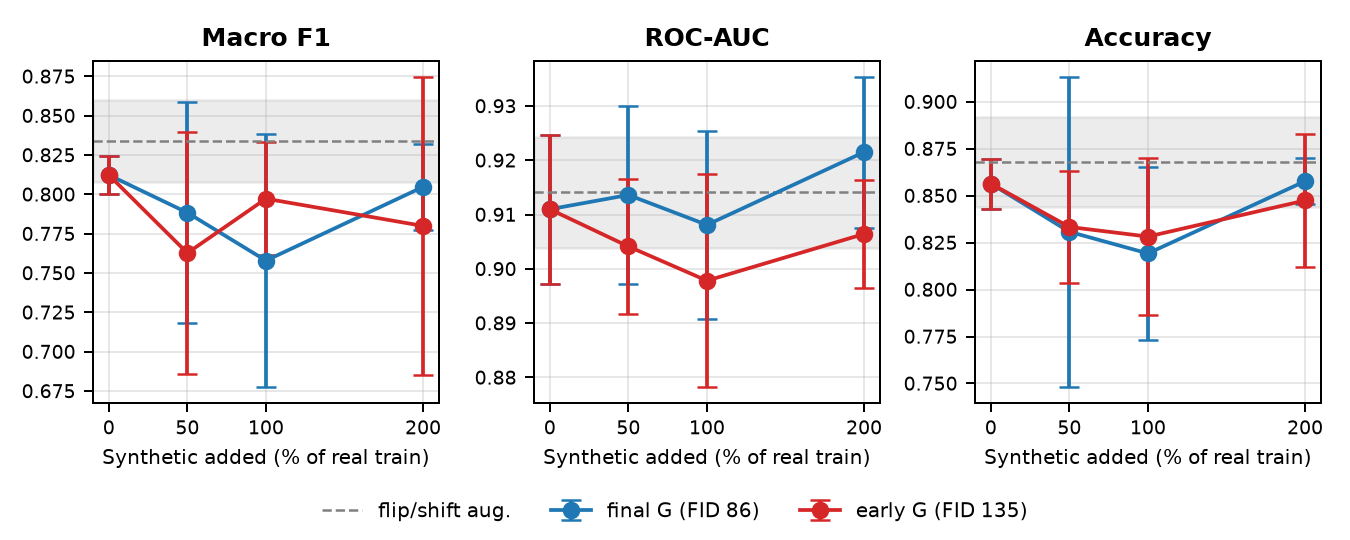
\includegraphics[width=\linewidth]{figures/breast_metrics_vs_ratio.png}
\caption{BreastMNIST: macro F1, ROC-AUC and accuracy against the amount of synthetic data (0\% = real only), for the
final (blue, FID 86) and early (red, FID 135) generator. Error bars: std over 5 seeds. Grey dashed line and band:
classical flip/shift augmentation (mean $\pm$ std).}
\label{fig:ratio}
\end{figure}

\begin{table}[htbp]
\centering
\caption{BreastMNIST per-class recall (mean over 5 seeds; from \texttt{confusion\_matrices.json}). The malignant class is
the clinically important minority class (42 test images).}
\label{tab:recall}
\small
\begin{tabular}{lcc}
\toprule
Setting & Malignant recall & Benign recall \\
\midrule
Real only           & 0.695 $\pm$ 0.085 & 0.916 \\
Real + flip/shift   & \textbf{0.771 $\pm$ 0.069} & 0.904 \\
+50\% GAN (final)   & 0.714 $\pm$ 0.181 & 0.874 \\
+100\% GAN (final)  & 0.662 $\pm$ 0.263 & 0.877 \\
+200\% GAN (final)  & 0.638 $\pm$ 0.106 & 0.939 \\
+100\% GAN (early)  & 0.810 $\pm$ 0.087 & 0.835 \\
GAN class balancing & 0.695 $\pm$ 0.124 & 0.926 \\
\bottomrule
\end{tabular}
\end{table}

\begin{figure}[htbp]
\centering
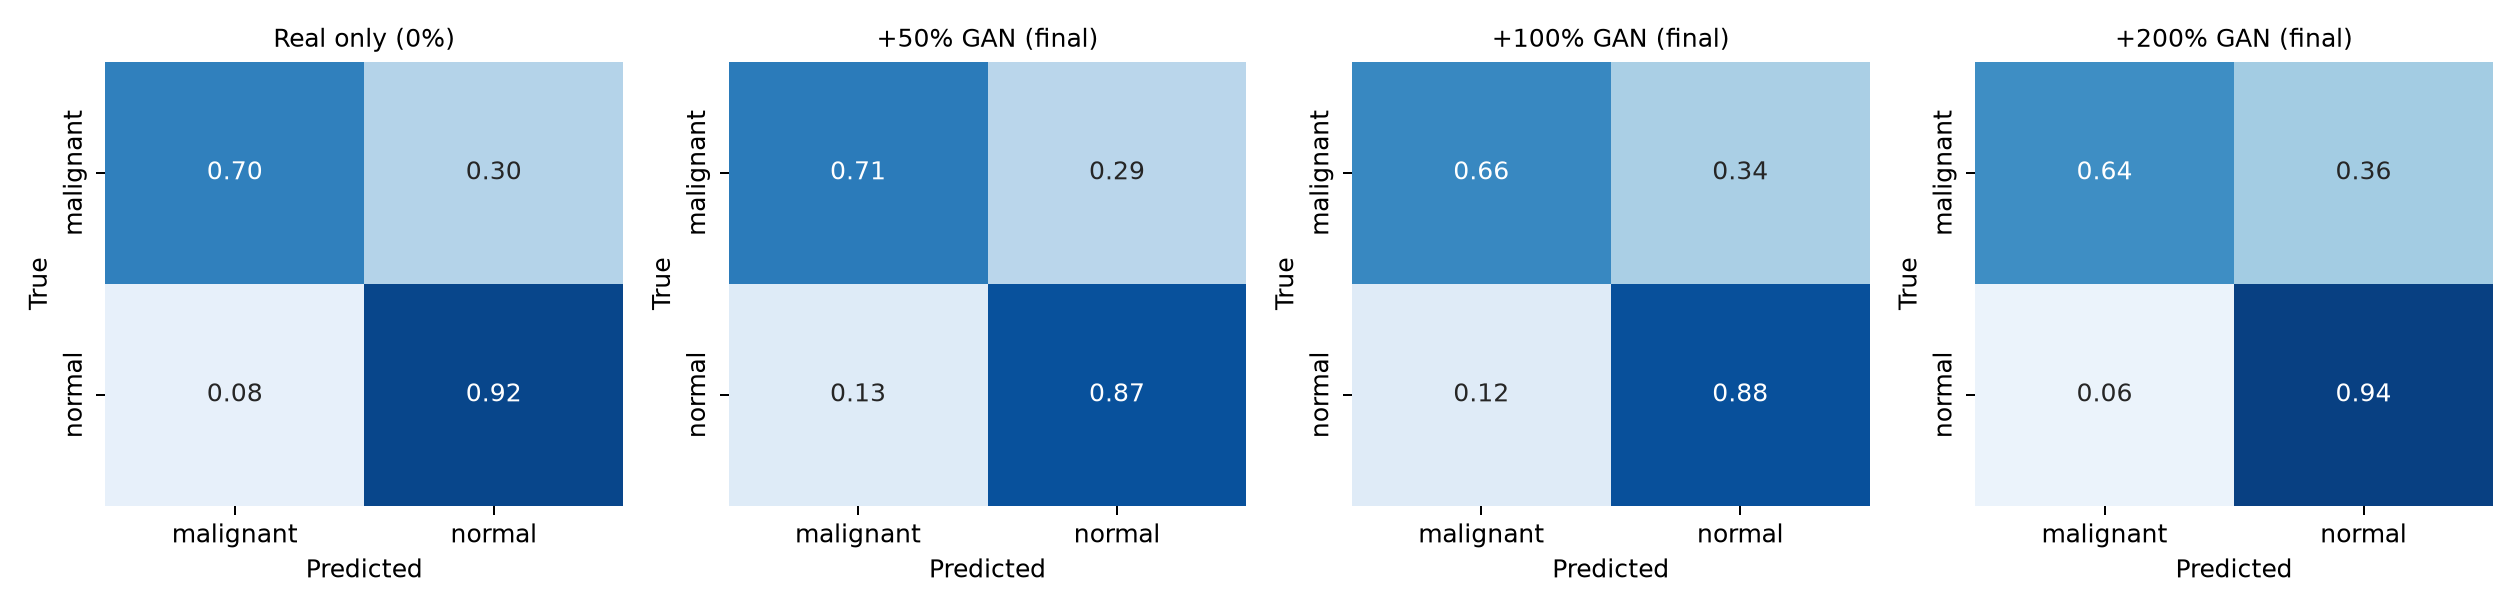
\includegraphics[width=\linewidth]{figures/breast_confusion.png}
\caption{BreastMNIST confusion matrices summed over 5 seeds and normalised per true class (diagonal = per-class recall)
for 0, 50, 100 and 200\% synthetic data from the final generator.}
\label{fig:confusion}
\end{figure}

\noindent The main observations are:
\begin{enumerate}
  \item \textbf{No GAN setting improves macro F1 over real-only training.} Mean F1 changes by between $-0.054$ and
        $+0.006$, and no difference is statistically significant (all $p>0.2$). Accuracy also does not improve
        (best: 0.864 with class balancing vs.\ 0.856).
  \item \textbf{Synthetic data makes training less stable.} The standard deviation of F1 over seeds grows from 0.012
        (real only) to as much as 0.095. With synthetic images in the training set the result depends much more on the
        random seed; e.g.\ one seed of +50\% (final) reached only 0.686 accuracy.
  \item \textbf{Quantity: the effect is not monotonic.} With the final generator, F1 first drops (50\%, 100\%) and then
        recovers almost to the baseline at 200\% (0.805). The +200\% setting gives the \emph{highest AUC} of all
        settings (0.922 vs.\ 0.911), i.e.\ slightly better ranking of cases, but it predicts ``benign'' more often:
        malignant recall falls to 0.638 while benign recall rises to 0.939 (Table~\ref{tab:recall}).
  \item \textbf{Quality matters for AUC.} At every ratio the better generator gives a higher AUC than the early one
        (0.914 vs.\ 0.904, 0.908 vs.\ 0.898, 0.922 vs.\ 0.906). Low-quality images (FID 135) lower AUC below the real-only
        baseline at every ratio. For F1 the picture is mixed and within the seed noise.
  \item \textbf{Classical augmentation is the strongest method.} Random flips and shifts give the best F1 (0.834,
        $+0.022$), the best accuracy (0.868) and raise malignant recall from 0.695 to 0.771 -- at no extra cost and with
        no generator. The difference is not significant at 5 seeds ($p=0.15$), but it is the only consistent positive trend.
  \item \textbf{GAN class balancing is neutral.} Adding 252 synthetic malignant images (to 399 vs.\ 399) leaves F1
        (0.819) and malignant recall (0.695) essentially unchanged: the synthetic minority images did not teach the
        classifier anything about malignant lesions that the 147 real ones did not.
\end{enumerate}

\FloatBarrier
\subsection{Second dataset: PneumoniaMNIST}
PneumoniaMNIST has nine times more real training images (4{,}708). Here the conditional DCGAN produces convincing chest
X-rays (Figure~\ref{fig:pneu_samples}): synthetic \emph{normal} images show clear lung fields and synthetic
\emph{pneumonia} images show hazy, opaque lungs, i.e.\ the class condition is respected. FID against 2{,}000 real training
images is 108.1 for the final and 193.3 for the early generator (real-vs-real reference: 25.3), and only
1.9\% of the generated images are closer to a training image than the closest 5\% of real test images -- fewer than
the 5\% expected for unseen real images, so again there is no memorisation. The quality gap is larger than on
BreastMNIST relative to the reference (108.1 vs.\ 25.3), even though the samples look convincing to the eye.

\begin{figure}[htbp]
\centering
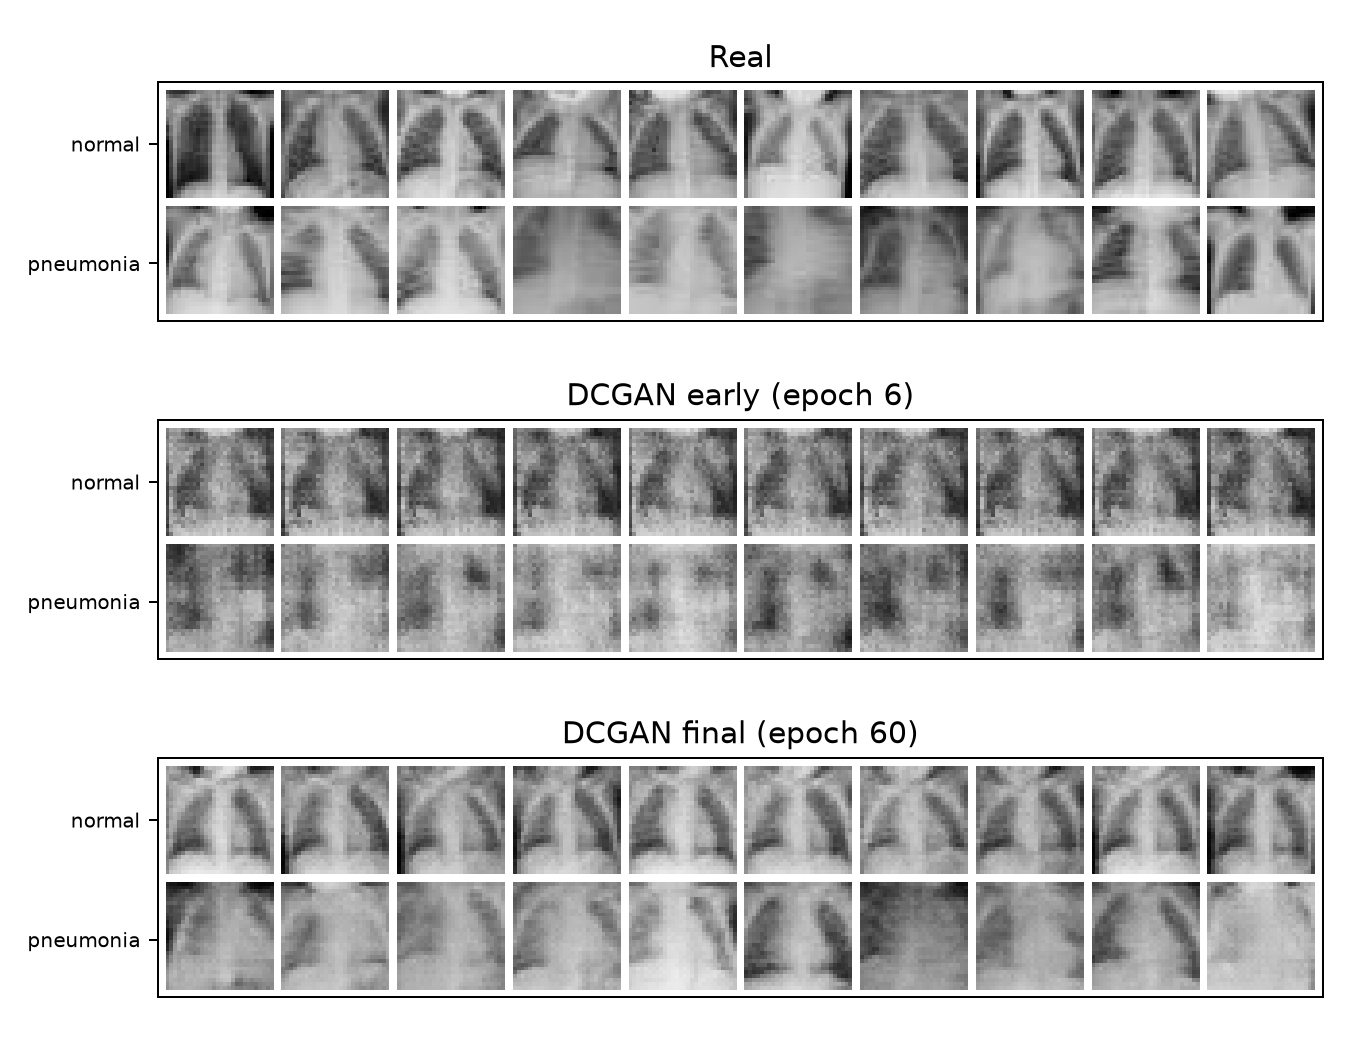
\includegraphics[width=0.9\linewidth]{figures/pneumonia_real_vs_synthetic.png}
\caption{PneumoniaMNIST: real training images (top), early generator after 6 epochs (middle), final generator after 60
epochs (bottom); one row per class.}
\label{fig:pneu_samples}
\end{figure}

\begin{table}[htbp]
\centering
\caption{PneumoniaMNIST, real test set (624 images), mean $\pm$ std over 3 seeds, 15 classifier epochs. $p$: Welch's
$t$-test on per-seed macro F1 vs.\ real only. Normal recall = recall of the minority class \emph{normal}.
Source: \texttt{results/pneumoniamnist/}.}
\label{tab:pneu}
\resizebox{\linewidth}{!}{%
\begin{tabular}{lcccccc}
\toprule
Setting & Accuracy & Macro F1 & AUC & Normal recall & $\Delta$F1 & $p$ \\
\midrule
Real only (0\%)     & \textbf{0.880 $\pm$ 0.017} & \textbf{0.861 $\pm$ 0.021} & 0.973 $\pm$ 0.006 & \textbf{0.691} & --       & --    \\
Real + flip/shift   & 0.808 $\pm$ 0.069 & 0.755 $\pm$ 0.104 & 0.972 $\pm$ 0.010 & 0.489 & $-$0.106 & 0.215 \\
\midrule
+50\% GAN (final)   & 0.860 $\pm$ 0.026 & 0.834 $\pm$ 0.035 & 0.973 $\pm$ 0.005 & 0.634 & $-$0.027 & 0.334 \\
+100\% GAN (final)  & 0.873 $\pm$ 0.006 & 0.853 $\pm$ 0.008 & 0.975 $\pm$ 0.002 & 0.668 & $-$0.008 & 0.573 \\
+200\% GAN (final)  & 0.875 $\pm$ 0.003 & 0.855 $\pm$ 0.004 & \textbf{0.976 $\pm$ 0.002} & 0.671 & $-$0.006 & 0.652 \\
+100\% GAN (early)  & 0.868 $\pm$ 0.005 & 0.845 $\pm$ 0.006 & 0.973 $\pm$ 0.001 & 0.651 & $-$0.016 & 0.317 \\
GAN class balancing & 0.863 $\pm$ 0.015 & 0.838 $\pm$ 0.019 & 0.973 $\pm$ 0.002 & 0.635 & $-$0.023 & 0.240 \\
\bottomrule
\end{tabular}}
\end{table}

\begin{figure}[htbp]
\centering
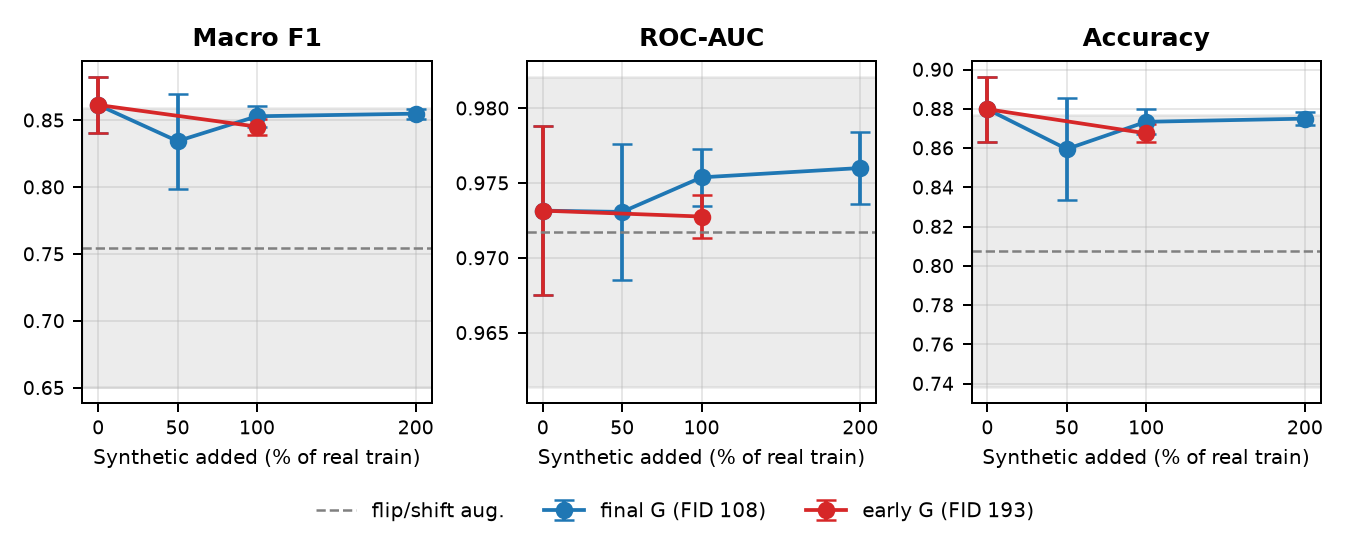
\includegraphics[width=\linewidth]{figures/pneumonia_metrics_vs_ratio.png}
\caption{PneumoniaMNIST: metrics against the amount of synthetic data. Note how the error bars shrink as more synthetic
images are added, while the means stay at the real-only level.}
\label{fig:pneu_ratio}
\end{figure}

\noindent Table~\ref{tab:pneu} and Figure~\ref{fig:pneu_ratio} show the same overall answer as on BreastMNIST, with two
instructive differences:
\begin{enumerate}
  \item \textbf{Again, no F1 gain.} No GAN setting beats the real-only baseline (F1 0.861); differences range from
        $-0.027$ to $-0.006$ and none is significant (all $p>0.2$). The real-only baseline (accuracy 0.880, AUC 0.973)
        is above the MedMNIST v2 ResNet-18 reference (0.854 / 0.944).
  \item \textbf{Synthetic data stabilises training here.} The seed-to-seed standard deviation of F1 falls from 0.021
        (real only) to 0.008 (+100\%) and 0.004 (+200\%), and the +200\% setting has the highest AUC (0.976). With a
        larger real set, the GAN is a better model of the data and its images act as a mild regulariser.
  \item \textbf{Quality still matters.} At +100\%, the final generator beats the early one on every metric (F1 0.853
        vs.\ 0.845, AUC 0.975 vs.\ 0.973, normal recall 0.668 vs.\ 0.651).
  \item \textbf{Classical augmentation hurts on chest X-rays.} Horizontal flipping drops F1 to 0.755 and normal recall to
        0.489. A mirrored chest X-ray puts the heart on the wrong side -- an anatomically impossible image -- whereas a
        mirrored breast ultrasound is still realistic. Augmentation must respect the anatomy of the modality.
  \item \textbf{All models under-detect the normal class.} Pneumonia recall is above 0.99 in every setting, but normal
        recall is only 0.49--0.69, so most errors are normal patients predicted as pneumonia. Neither proportional
        augmentation nor GAN class balancing (normal recall 0.635) fixed this.
\end{enumerate}

% -------------------------------------------------------------------------------------
\FloatBarrier
\section{Discussion}
\textbf{Answer to the research question.} In our setting, adding DCGAN-generated images did \emph{not} improve a CNN
classifier on real test images, on either dataset, at any amount (50--200\%) or quality (FID 86 vs.\ 135). This
differs from the improvement reported by Frid-Adar et al.~\cite{fridadar2018gan}, and we see four reasons in our results.

\begin{enumerate}
  \item \textbf{A GAN cannot add information it never saw.} The generator is trained on the same 546 (or 4{,}708)
        images as the classifier. Our memorisation check shows that it does not copy them, but the samples are
        variations of the same visual content -- with limited diversity (near-duplicate samples, Figure~\ref{fig:nn}).
        New \emph{information} about rare cases (e.g.\ unusual malignant lesions) can only come from new real data.
  \item \textbf{The quality gap acts like label noise.} With FID 86 against a real-vs-real floor of 59, part of the
        synthetic images are not clearly typical of their class. When such images make up a third to two thirds of the
        training set, the classifier partly learns GAN artefacts and ambiguous class boundaries; on BreastMNIST this
        shows up as a lower and less stable F1 at 50--100\%.
  \item \textbf{Quantity helps ranking more than decisions.} At 200\%, AUC is the best of all settings on both datasets
        (0.922 and 0.976), so synthetic images seem to regularise the learned features; but the decision threshold
        shifts towards the majority class (malignant recall 0.638). A threshold tuned on validation data might
        turn this AUC gain into an F1 gain -- a cheap follow-up experiment.
  \item \textbf{Better images help, but not enough.} The final generator beats the early one in AUC at every BreastMNIST
        ratio and on every PneumoniaMNIST metric, so quality clearly matters; the trend suggests that a stronger
        generator (StyleGAN2-ADA, diffusion) is a prerequisite for gains, not an option.
\end{enumerate}

\textbf{Dataset size changes the role of synthetic data.} With 546 images, synthetic data mainly added variance; with
4{,}708 images it reduced variance (std of F1 from 0.021 to 0.004). A GAN trained on more data is a better model of
that data, and its samples then behave like a smooth regulariser rather than noise.

\textbf{Classical augmentation must match the modality.} Simple flips and shifts were the best method for breast
ultrasound (F1 +0.022, malignant recall +0.076) but the worst for chest X-rays (F1 $-0.106$), because a mirrored chest is
anatomically wrong. Domain knowledge matters more than the sophistication of the augmentation method.

\textbf{Why multiple seeds were essential.} With a single seed we could have reported almost any conclusion: individual
BreastMNIST runs of +50\% GAN range from accuracy 0.686 to 0.891. Only the mean over seeds, the standard deviation and the
$t$-test reveal that none of the differences is reliable -- a methodological point that much of the GAN-augmentation
literature does not address.

\textbf{Practical recommendation.} For a small medical dataset, first use modality-appropriate classical augmentation and
report results over several seeds; consider GAN augmentation only with a generator whose FID is close to the real-vs-real
floor, check it for memorisation, and evaluate it against the classical baseline as done here.

\section{Limitations and Future Work}
\begin{itemize}
  \item \textbf{Resolution.} We used 28$\times$28 images to fit a CPU budget; fine lesion details are lost. MedMNIST+ offers
        64--224\,px versions on which both the GAN and the classifier could behave differently.
  \item \textbf{Generator family.} DCGAN is a 2016 architecture. StyleGAN2-ADA or diffusion models produce markedly better
        samples on small datasets and may change the conclusion.
  \item \textbf{Metric mismatch.} FID relies on ImageNet features that are poorly suited to grayscale ultrasound; a
        medical-domain feature extractor would give a more meaningful quality score.
  \item \textbf{Statistics.} Five (three) seeds give a rough estimate of variance; the BreastMNIST test set has only
        42 malignant images, so a single changed prediction moves recall by 2.4 points.
  \item \textbf{Single classifier.} We used one small CNN; a larger or pretrained model may benefit differently from
        synthetic data.
  \item \textbf{No clinical validation.} Synthetic images were not reviewed by radiologists; the system is a research
        prototype, not a diagnostic tool.
\end{itemize}

\section{Conclusion}
We built a complete, reproducible pipeline to test whether GAN-generated images help a classifier trained on a small
medical dataset. A class-conditional DCGAN with DiffAugment-style translation learned realistic-looking breast ultrasound
and chest X-ray images without memorising its training data, and a better generator (lower FID) consistently gave better
classifiers than a worse one. Nevertheless, adding 50--200\% synthetic images did not improve macro F1 on real test
images for either dataset, and no difference was statistically significant over 5 (3) seeds. Synthetic data raised AUC
slightly at 200\% and, on the larger dataset, made training much more stable, while simple flip/shift augmentation was the
best method for ultrasound but harmful for chest X-rays. The answer to ``does synthetic data help?'' is therefore:
\emph{not by itself with a DCGAN at this scale -- quality, dataset size and the choice of baseline decide}.
Future work: higher resolution (MedMNIST+), stronger generators (StyleGAN2-ADA, diffusion), threshold tuning, and
filtering synthetic images by classifier confidence before adding them.

\section*{Code Availability and Demo}
Code, results and instructions: \url{https://github.com/Bhagwati23/GAN-medicalAugmentation}. The package \texttt{ganaug}
contains one module per stage (data, DCGAN, GAN training, augmentation, classifier, FID, experiments, report figures);
\texttt{tests/} checks shapes, determinism and that synthetic images never reach the validation or test sets; a GitHub
Actions workflow runs these tests on every pull request. \texttt{app.py} is a Gradio web app that generates synthetic images
for a chosen class and generator checkpoint, classifies an uploaded or real test image with both the real-only and the
GAN-augmented classifier side by side, and shows the result tables.

\section*{Individual Contributions}
\begin{itemize}
  \item \textbf{Arjun Kadam} (su-24022@sitare.org): synthetic-data augmentation pipeline (issue \#5), integration, testing,
        CI and reproducibility (\#8), demo application, project report (\#9).
  \item \textbf{Bhagwati} (su-24032@sitare.org): conditional DCGAN architecture (\#3), GAN training, checkpoints and samples (\#4), independent re-run of GAN training (reproducibility check);
        repository set-up, issue planning, team workflow, and PR review and merge coordination.
  \item \textbf{Maneesh Sakhwar} (su-24068@sitare.org): dataset selection, loading, exploration notebook and data-leakage tests (\#1); FID/KID evaluation
        and memorisation check (\#6).
  \item \textbf{Anand Singh} (su-24014@sitare.org): CNN baseline (\#2); experiment runs, comparison tables and figures (\#7).
\end{itemize}

.
% Every number comes from results/ in the repository (see the table/figure captions).
% =====================================================================================

\begin{abstract}
Medical image datasets are often small and class-imbalanced, which limits how well deep classifiers can be trained.
We study whether images generated by a Generative Adversarial Network (GAN) can make up for this.
We train a class-conditional DCGAN on the training split of BreastMNIST (546 breast ultrasound images, 27\% malignant)
and add 0, 50, 100 or 200\% synthetic images to the training set of a CNN classifier, which is always evaluated on the
same held-out set of \emph{real} test images. To separate the effect of the \emph{amount} of synthetic data from its
\emph{quality}, we repeat every experiment with an early generator checkpoint (FID 134.9) and the fully trained
generator (FID 86.4; the real-vs-real reference is 59.1), compare against classical flip/shift augmentation and
against GAN-based class balancing, run five random seeds per setting, and test significance with Welch's $t$-test.
The generator learns realistic images without memorising the training set, and the better generator consistently beats
the worse one. Yet no amount of synthetic data improves macro F1 over real-only training (0.812; changes from $-0.054$ to
$+0.006$, none significant), while simple flip/shift augmentation gives the best F1 (0.834). Adding 200\% synthetic images
yields the highest AUC (0.922 vs.\ 0.911) but lowers malignant recall.
A second, nine times larger dataset (PneumoniaMNIST) is used to check whether the conclusion depends on dataset size.
All code, results and an interactive demo are available at \url{https://github.com/Bhagwati23/GAN-medicalAugmentation}.

\vspace{0.5cm}
\noindent
{\em Key Words}: Generative Adversarial Networks, DCGAN, Data Augmentation, Medical Image Classification,
Synthetic Data, MedMNIST, FID.
\end{abstract}
\hrulefill

% -------------------------------------------------------------------------------------
\section{Introduction}
Deep convolutional networks need many labelled examples, but labelled medical images are expensive: they require
expert annotation, are protected by privacy rules, and positive (disease) cases are rare. The usual remedy is
\emph{data augmentation}: creating new training examples from existing ones. Classical augmentation applies simple
geometric or photometric transforms (flips, shifts, rotations, contrast changes)~\cite{shorten2019survey}. Generative
Adversarial Networks (GANs)~\cite{goodfellow2014gan} offer a more ambitious option: learn the distribution of the
training images and sample entirely new ones. Frid-Adar et al.~\cite{fridadar2018gan} reported that GAN-generated
liver-lesion images raised CNN sensitivity and specificity, which made GAN augmentation popular in medical
imaging~\cite{yi2019ganmedical}.

However, a GAN trained on a small dataset only sees the same few hundred images as the classifier. It is therefore not
obvious that its samples add \emph{new information}; they may only add noise, or copies of the training images.
This project asks a precise question:

\begin{quote}
\emph{When a classifier is trained on a small medical dataset, does adding GAN-generated images improve its performance
on real, unseen images -- and how does the gain depend on the amount and on the quality of the synthetic data?}
\end{quote}

\noindent\textbf{Contributions.}
\begin{itemize}
  \item A reproducible pipeline (MedMNIST v2 data, class-conditional DCGAN, augmentation at 0/\allowbreak 50/\allowbreak 100/\allowbreak 200\%, CNN
        classifier, FID/KID evaluation) with strict separation of training, validation and test data.
  \item A two-axis study: \emph{quantity} (four synthetic ratios) $\times$ \emph{quality} (early vs.\ final generator,
        measured by FID and KID), plus two reference points: classical flip/shift augmentation and GAN class balancing.
  \item Statistical care: five seeds per setting, mean $\pm$ standard deviation, Welch's $t$-test against the real-only baseline.
  \item Checks that the generator does not simply memorise the training set (nearest-neighbour distances and latent
        interpolation).
  \item A replication on a second, larger dataset (PneumoniaMNIST) and an interactive web demo.
\end{itemize}

\begin{keybox}{Key findings at a glance}
\begin{itemize}
  \item \textbf{No F1 gain from GAN images} on either dataset at 50, 100 or 200\% synthetic data (BreastMNIST real-only
        F1 0.812 vs.\ 0.758--0.819 with GAN data; none significant, all $p>0.2$).
  \item \textbf{Quality matters:} the better generator (FID 86) beats the early one (FID 135) in AUC at every ratio.
  \item \textbf{200\% synthetic gives the best AUC} on both datasets (0.922 and 0.976) and, on the larger dataset,
        cuts seed-to-seed variance five-fold.
  \item \textbf{No memorisation:} no generated image is closer to a training image than typical unseen real images.
  \item \textbf{Classical augmentation depends on anatomy:} best for breast ultrasound (F1 0.834), harmful for chest
        X-rays (F1 0.755) because mirrored chests are anatomically wrong.
\end{itemize}
\end{keybox}

% -------------------------------------------------------------------------------------
\section{Related Work}
\textbf{GANs and DCGAN.} A GAN~\cite{goodfellow2014gan} trains a generator $G$ to map random noise $z$ to images and a
discriminator $D$ to tell real from generated images; the two are trained against each other. DCGAN~\cite{radford2016dcgan}
gave architectural rules that make this training stable for images: strided (transposed) convolutions instead of pooling,
batch normalisation, ReLU in $G$, LeakyReLU in $D$, Adam with learning rate $2\times10^{-4}$ and $\beta_1=0.5$.
Conditional GANs~\cite{mirza2014cgan} feed the class label to both networks so that images of a chosen class can be requested.

\textbf{GANs with little data.} With few training images the discriminator quickly memorises them and stops giving
useful gradients. DiffAugment~\cite{zhao2020diffaugment} applies the same random, differentiable augmentation to real and
generated images before the discriminator, which strongly improves GANs trained on a few hundred images.

\textbf{GAN augmentation in medical imaging.} Frid-Adar et al.~\cite{fridadar2018gan} generated liver-lesion CT patches
with DCGAN and improved classification from 78.6\% to 85.7\% sensitivity. Reviews~\cite{yi2019ganmedical} report
mixed results in later work, often without multiple seeds or a comparison with classical augmentation -- gaps this
project addresses.

\textbf{Evaluating generated images.} The Fr\'echet Inception Distance (FID)~\cite{heusel2017fid} compares Inception-v3
feature statistics of real and generated images; the Kernel Inception Distance (KID)~\cite{binkowski2018kid} is an
unbiased alternative better suited to small samples. Ravuri and Vinyals~\cite{ravuri2019cas} showed that such scores do not
fully predict how useful samples are for training a classifier -- which is exactly what our classifier experiments measure.

\textbf{MedMNIST.} MedMNIST v2~\cite{yang2023medmnist} provides standardised, pre-split 28$\times$28 biomedical datasets with
benchmark results, which makes our numbers comparable and reproducible.

% -------------------------------------------------------------------------------------
\section{Datasets}
We use two binary datasets from MedMNIST v2~\cite{yang2023medmnist} at their default 28$\times$28 grayscale resolution and
keep the \emph{official} train/validation/test splits (Table~\ref{tab:data}, Fig.~\ref{fig:data}).

\textbf{BreastMNIST} (main dataset) is derived from a breast ultrasound dataset~\cite{aldhabyani2020busi}; the label is
\emph{malignant} (class 0) or \emph{normal/benign} (class 1). With only 546 training images and 27\% malignant cases it is
exactly the small, imbalanced setting in which synthetic data is supposed to help.

\textbf{PneumoniaMNIST} (second dataset) is derived from paediatric chest X-rays~\cite{kermany2018pneumonia}: \emph{normal}
(class 0) vs.\ \emph{pneumonia} (class 1), with 4{,}708 training images (about nine times more). It tells us whether a
conclusion drawn on BreastMNIST changes when real data is more plentiful.

\begin{table}[htbp]
\centering
\caption{Official MedMNIST v2 splits (images per class). Source: \texttt{results/dataset\_stats.json}.}
\label{tab:data}
\begin{tabular}{llrrr}
\toprule
Dataset & Class & Train & Val & Test \\
\midrule
BreastMNIST    & malignant      & 147   & 21  & 42  \\
               & normal/benign  & 399   & 57  & 114 \\
               & \emph{total}   & 546   & 78  & 156 \\
\midrule
PneumoniaMNIST & normal         & 1{,}214 & 135 & 234 \\
               & pneumonia      & 3{,}494 & 389 & 390 \\
               & \emph{total}   & 4{,}708 & 524 & 624 \\
\bottomrule
\end{tabular}
\end{table}

\begin{figure}[htbp]
\centering
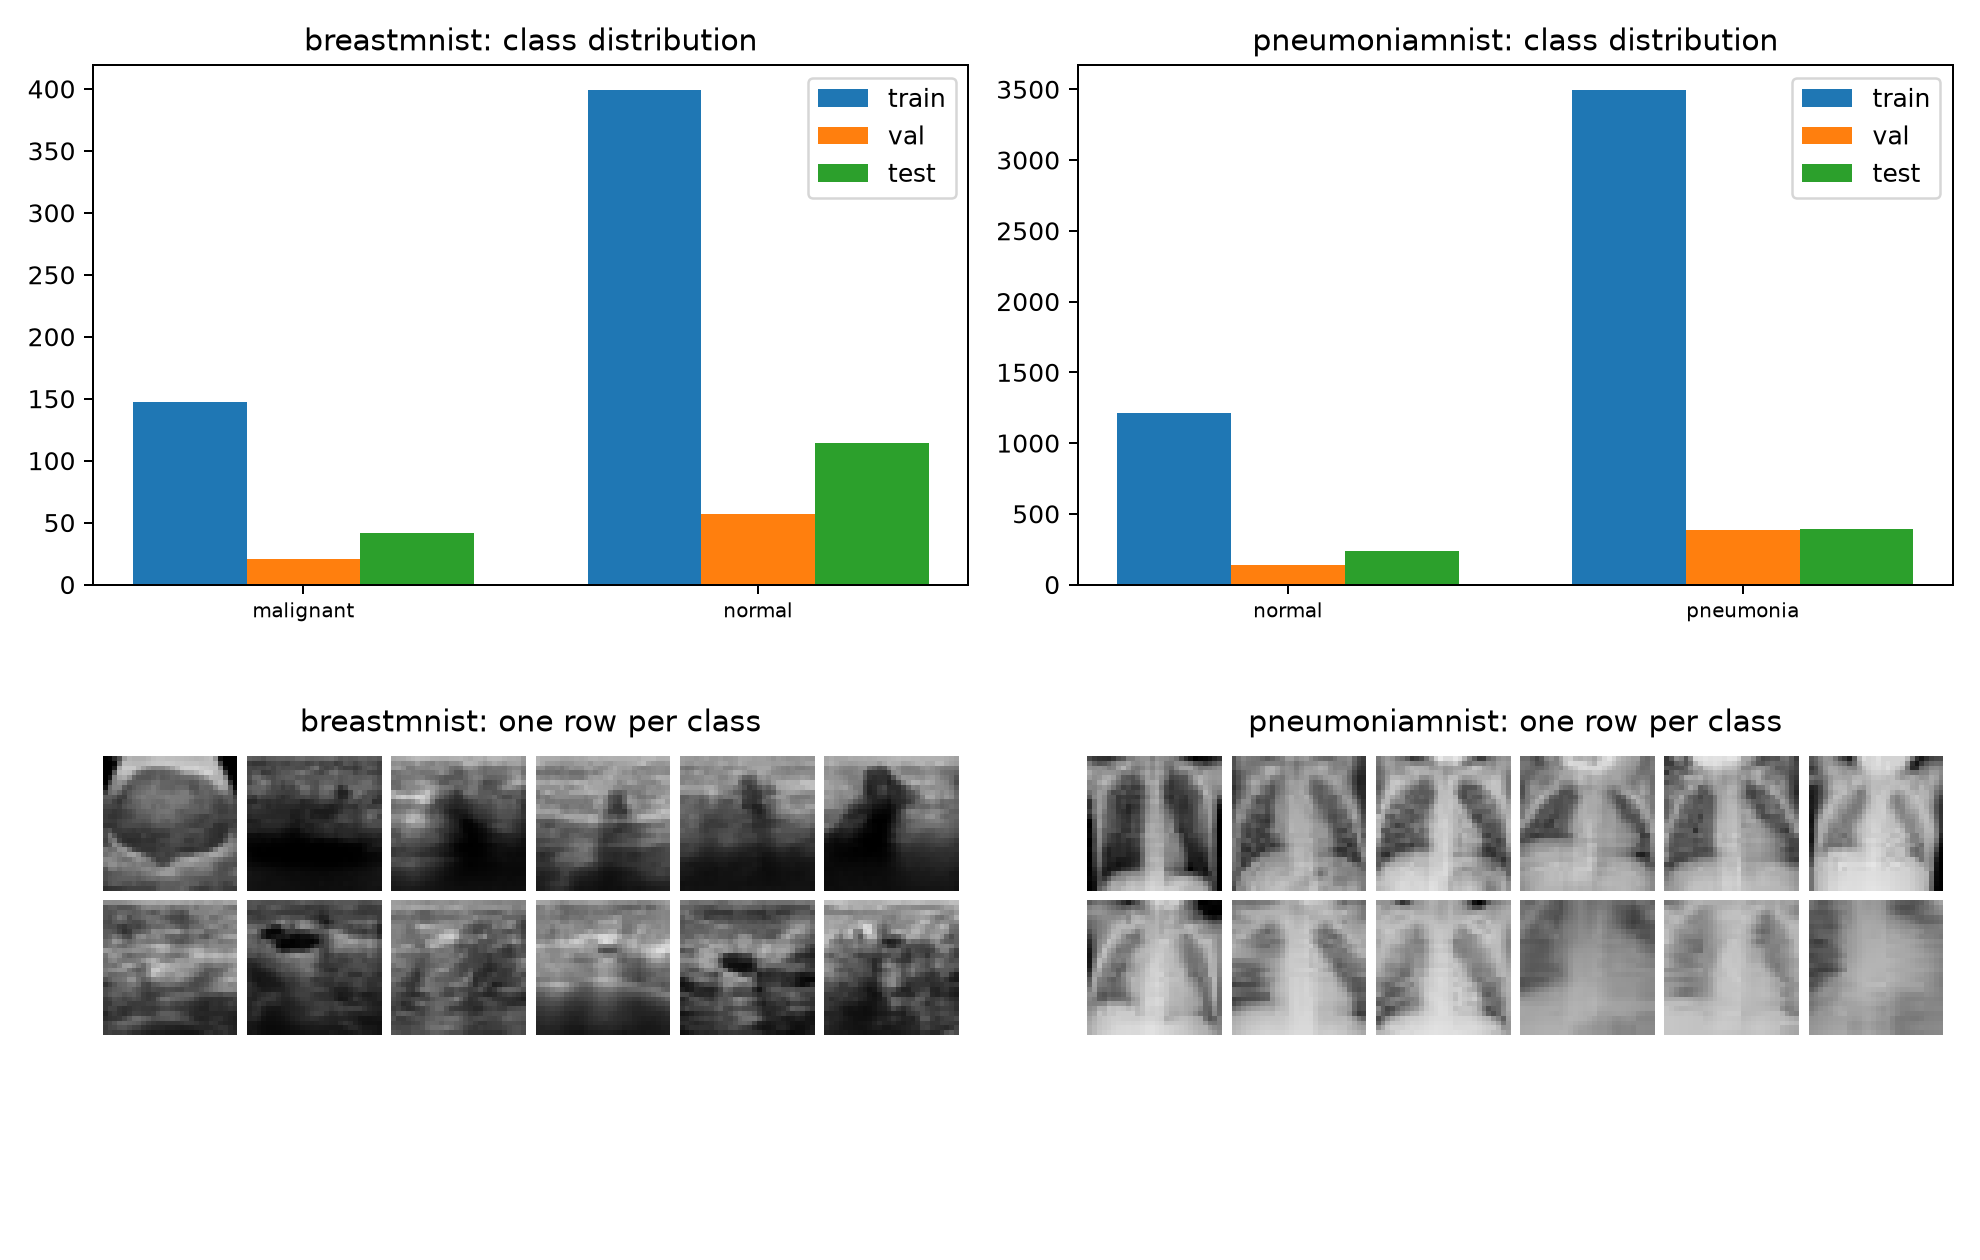
\includegraphics[width=\linewidth]{figures/dataset_overview.png}
\caption{Class distribution per split (top) and training images, one row per class (bottom). Both datasets are imbalanced
(minority class: malignant in BreastMNIST, normal in PneumoniaMNIST).}
\label{fig:data}
\end{figure}

\textbf{Preprocessing and leakage control.} Pixel values are scaled from $[0,255]$ to $[-1,1]$, the output range of the
generator's $\tanh$. The GAN is trained \emph{only} on the training split. Synthetic images are added \emph{only} to the
training split. Validation (used to choose the best epoch) and test (used once, for the final numbers) contain only real
images and are identical in every experiment. These rules are enforced in code and checked by unit tests.

% -------------------------------------------------------------------------------------
\section{Method}

\subsection{Pipeline}
\begin{enumerate}
  \item Train a class-conditional DCGAN on the real training images; save an \emph{early} checkpoint (after 10\% of
        training) and the \emph{final} one.
  \item Score both generators with FID and KID against the real training images, and check for memorisation.
  \item For each setting (Section~\ref{sec:settings}), build a training set of real images plus a controlled number of
        synthetic images, train the CNN classifier with five seeds, and evaluate on the real test set.
  \item Compare every setting with the real-only baseline (mean, standard deviation, Welch's $t$-test).
\end{enumerate}

\subsection{Class-conditional DCGAN}
Table~\ref{tab:gan} lists the architecture. The generator concatenates a 100-dimensional Gaussian noise vector $z$ with a
learned 50-dimensional embedding of the class label $y$, projects it to a $256\times7\times7$ tensor and upsamples it with
two stride-2 transposed convolutions to $28\times28$. The discriminator receives the image together with a learned
$28\times28$ ``label map'' as a second channel, so it judges whether the image is realistic \emph{for that class}.
Following DCGAN~\cite{radford2016dcgan}, weights are initialised from $\mathcal{N}(0,0.02)$, $G$ uses BatchNorm + ReLU and
$D$ uses LeakyReLU(0.2), no pooling layers.

\begin{table}[htbp]
\centering
\caption{Conditional DCGAN architecture (\texttt{ganaug/dcgan.py}). ConvT = transposed convolution, k = kernel, s = stride.}
\label{tab:gan}
\small
\begin{tabular}{ll}
\toprule
\multicolumn{2}{l}{\textbf{Generator} (2.56\,M parameters)} \\
Input & $z\in\mathbb{R}^{100}$ $\oplus$ Embedding$(y)\in\mathbb{R}^{50}$ \\
Linear + BN + ReLU & $150 \rightarrow 256\times7\times7$ \\
ConvT k4 s2 + BN + ReLU & $\rightarrow 128\times14\times14$ \\
ConvT k4 s2 + BN + ReLU & $\rightarrow 64\times28\times28$ \\
Conv k3 s1 + $\tanh$ & $\rightarrow 1\times28\times28$, values in $[-1,1]$ \\
\midrule
\multicolumn{2}{l}{\textbf{Discriminator} (0.43\,M parameters)} \\
Input & image $\oplus$ label map $\rightarrow 2\times28\times28$ \\
Conv k4 s2 + LeakyReLU & $\rightarrow 64\times14\times14$ \\
Conv k4 s2 + BN + LeakyReLU & $\rightarrow 128\times7\times7$ \\
Conv k3 s2 + BN + LeakyReLU & $\rightarrow 256\times4\times4$ \\
Dropout(0.3) + Linear & $\rightarrow$ 1 logit (real/fake) \\
\bottomrule
\end{tabular}
\end{table}

\textbf{Training objective.} With $\sigma$ the sigmoid and $\tilde{x}=T(x)$ a random translation (below), $D$ minimises
\begin{equation}
\mathcal{L}_D = -\,\mathbb{E}_{x,y}\big[\,0.9\log\sigma(D(\tilde{x},y))\big] - \mathbb{E}_{z,y}\big[\log\big(1-\sigma(D(\widetilde{G(z,y)},y))\big)\big],
\end{equation}
and $G$ minimises the non-saturating loss $\mathcal{L}_G = -\,\mathbb{E}_{z,y}\big[\log\sigma(D(\widetilde{G(z,y)},y))\big]$.
Two additions help with only 546 training images:
(i) \emph{one-sided label smoothing}: the target for real images is 0.9 instead of 1, so $D$ does not become over-confident;
(ii) \emph{DiffAugment-style translation}~\cite{zhao2020diffaugment}: every real and generated image is shifted by a random
$-2\ldots2$ pixels (edge-replicate padding) before it is shown to $D$, which keeps $D$ from memorising the training images.
Both networks use Adam ($2\times10^{-4}$, $\beta=(0.5,0.999)$), batch size 64.

\subsection{Augmentation protocol}
\label{sec:aug}
For a ratio $r\in\{0, 0.5, 1, 2\}$ we add $\mathrm{round}(r\cdot n_c)$ synthetic images of each class $c$, where $n_c$ is
the number of real training images of class $c$. This keeps the real class ratio (for BreastMNIST: $+50\%$ = 274,
$+100\%$ = 546, $+200\%$ = 1{,}092 synthetic images). For each generator we sample one fixed pool of synthetic images
(fixed seed) and every ratio takes the first $k$ images of each class, so the sets are \emph{nested}
($50\% \subset 100\% \subset 200\%$): differences between ratios come from the amount of data, not from a luckier draw.
In the \emph{class-balancing} setting we instead add only minority-class images until both classes have the same size
(BreastMNIST: 252 synthetic malignant images, giving 399 vs.\ 399).

\subsection{Classifier}
All settings use the same CNN (\texttt{ganaug/cnn.py}, 0.29\,M parameters): three blocks of
[Conv3$\times$3--BN--ReLU]$\times$2 + MaxPool with 32, 64 and 128 channels ($28\to14\to7\to3$), global average pooling,
dropout 0.3 and a linear layer. It is trained with cross-entropy, AdamW (learning rate $10^{-3}$, weight decay $10^{-4}$),
a cosine learning-rate schedule and batch size 64. After each epoch we compute the validation ROC-AUC and keep the weights
with the best value (model selection on validation, never on test). The model is deliberately small: the dataset is tiny
and all experiments ran on a CPU. Our real-only baseline (Section~\ref{sec:results}) is in line with the ResNet-18 results
reported by MedMNIST v2~\cite{yang2023medmnist} (BreastMNIST, 28$\times$28: accuracy 0.863, AUC 0.901).

\subsection{Evaluation}
\textbf{Classifier metrics} (real test set): accuracy; \emph{macro} precision, recall and F1 (each class weighted
equally, so missing the minority class is penalised; macro recall equals balanced accuracy); ROC-AUC (threshold-free
ranking quality); and confusion matrices. Macro F1 is our main metric because accuracy can look good on imbalanced data
by mostly predicting the majority class.

\textbf{Image quality.} FID and KID are computed with \texttt{torch-fidelity} between the real training images and the
same number of generated images with the same class ratio (images converted to 3-channel uint8 and resized to
299$\times$299 for Inception-v3). Because 28$\times$28 grayscale ultrasound images are very different from ImageNet photos,
absolute FID values are not comparable to natural-image papers; we therefore also report FID between the real training and
real test images as a \emph{reference floor}.

\textbf{Memorisation check.} For every generated image we find the closest real training image (pixel $L_2$ distance) and
compare these distances with the same distances for real \emph{test} images, which are realistic but unseen. A generator
that copies training images would produce many samples closer to the training set than almost any real test image; we
report the fraction of generated images closer than the 5th percentile of the test distances (about 0.05 is expected if
there is no copying).

\textbf{Statistics.} Each setting is trained with seeds 0--4 (BreastMNIST) or 0--2 (PneumoniaMNIST); we report mean
$\pm$ standard deviation and a two-sided Welch's $t$-test of the per-seed macro F1 against the real-only baseline.

% -------------------------------------------------------------------------------------
\section{Experimental Setup}
\label{sec:settings}
\begin{table}[htbp]
\centering
\caption{Experiment settings. Only the training set changes; the CNN, its hyper-parameters, and the validation and test
sets are identical everywhere.}
\label{tab:settings}
\small
\begin{tabular}{lp{5.2cm}}
\toprule
Setting & Training data \\
\midrule
Real only (0\%) & real training images (baseline) \\
Real + flip/shift & real images, random horizontal flip and $\pm2$\,px shift on the fly \\
+50/100/200\% GAN (final) & real + synthetic from the final generator \\
+50/100/200\% GAN (early) & real + synthetic from the early generator \\
GAN class balancing & real + synthetic minority-class images until classes are equal \\
\bottomrule
\end{tabular}
\end{table}

\begin{table}[htbp]
\centering
\caption{Training configuration.}
\label{tab:hparams}
\small
\begin{tabular}{lll}
\toprule
 & BreastMNIST & PneumoniaMNIST \\
\midrule
GAN epochs (updates)       & 300 (2{,}400) & 60 (4{,}380) \\
Early checkpoint           & epoch 30      & epoch 6 \\
Classifier epochs          & 40            & 15 \\
Seeds per setting          & 5             & 3 \\
Settings run               & all 9         & 7 (no early 50/200\%) \\
FID sample size            & 546           & 2{,}000 (random subset) \\
\bottomrule
\end{tabular}
\end{table}

All experiments ran on a laptop CPU with PyTorch. Table~\ref{tab:settings} lists the settings and Table~\ref{tab:hparams}
the configuration. Because PneumoniaMNIST is nine times larger, we used fewer classifier epochs, seeds and settings for it.
Everything is reproduced by \texttt{bash run\_all.sh}.

% -------------------------------------------------------------------------------------
\FloatBarrier
\section{Results}
\label{sec:results}

\subsection{Quality of the synthetic images}
\textbf{Training dynamics.} Figure~\ref{fig:losses} shows that GAN training on BreastMNIST stayed balanced for all 300
epochs: the discriminator loss stays close to $2\ln 2\approx1.39$ (the value when $D$ cannot separate real from fake), and
at the end $D$ assigns on average 0.46 to real and 0.44 to generated images. There is no sign of mode collapse (where
$D(G(z))$ would drop to 0 and all samples would look alike) or of $D$ winning outright.

\textbf{Reproducibility of GAN training.} The GAN training was run twice, independently, on two different laptops with
the same code, configuration and seed: run~1 produced the generators used for every experiment in this report, and run~2
(by Bhagwati, committed as the training log in \texttt{results/}) checks that training can be repeated. Averaged over the
last 10\% of epochs, the two runs agree closely: BreastMNIST discriminator loss 1.371 vs.\ 1.377, $D(x)$ 0.459 vs.\ 0.456
and $D(G(z))$ 0.441 vs.\ 0.444; PneumoniaMNIST discriminator loss 1.376 vs.\ 1.377, $D(x)$ 0.455 vs.\ 0.456. Bit-exact
equality is not expected, because CPU floating-point operations are not deterministic across machines and library
versions, but the training reaches the same balanced state.

\begin{figure}[htbp]
\centering
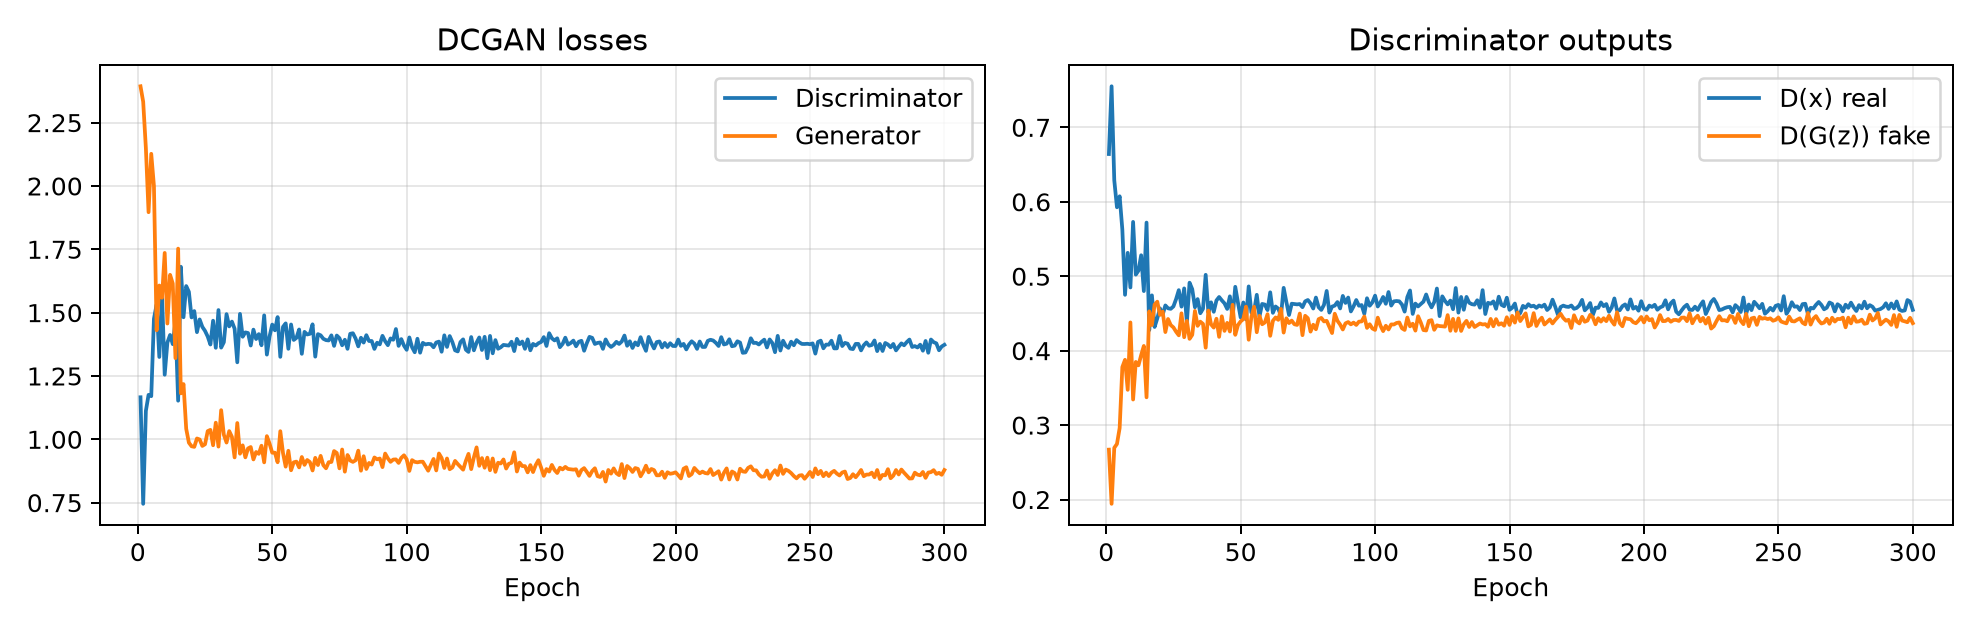
\includegraphics[width=\linewidth]{figures/breast_gan_losses.png}
\caption{DCGAN training on BreastMNIST. Left: losses. Right: mean discriminator output for real ($D(x)$) and generated
($D(G(z))$) images; both stay close to 0.5, i.e.\ a balanced adversarial game. Source: \texttt{results/breastmnist/report\_run/gan\_losses.csv} (run~1).}
\label{fig:losses}
\end{figure}

\textbf{Visual quality.} Figure~\ref{fig:samples} compares real images with samples from both generators. After 30 epochs
the generator only reproduces the global layout (bright tissue at the top, dark region at the bottom) with heavy noise.
After 300 epochs the samples contain lesion-like dark regions and ultrasound speckle texture; synthetic \emph{malignant}
images tend to show larger, darker, irregular masses, matching the real malignant row. Small checkerboard artefacts from
the transposed convolutions remain.

\begin{figure}[htbp]
\centering
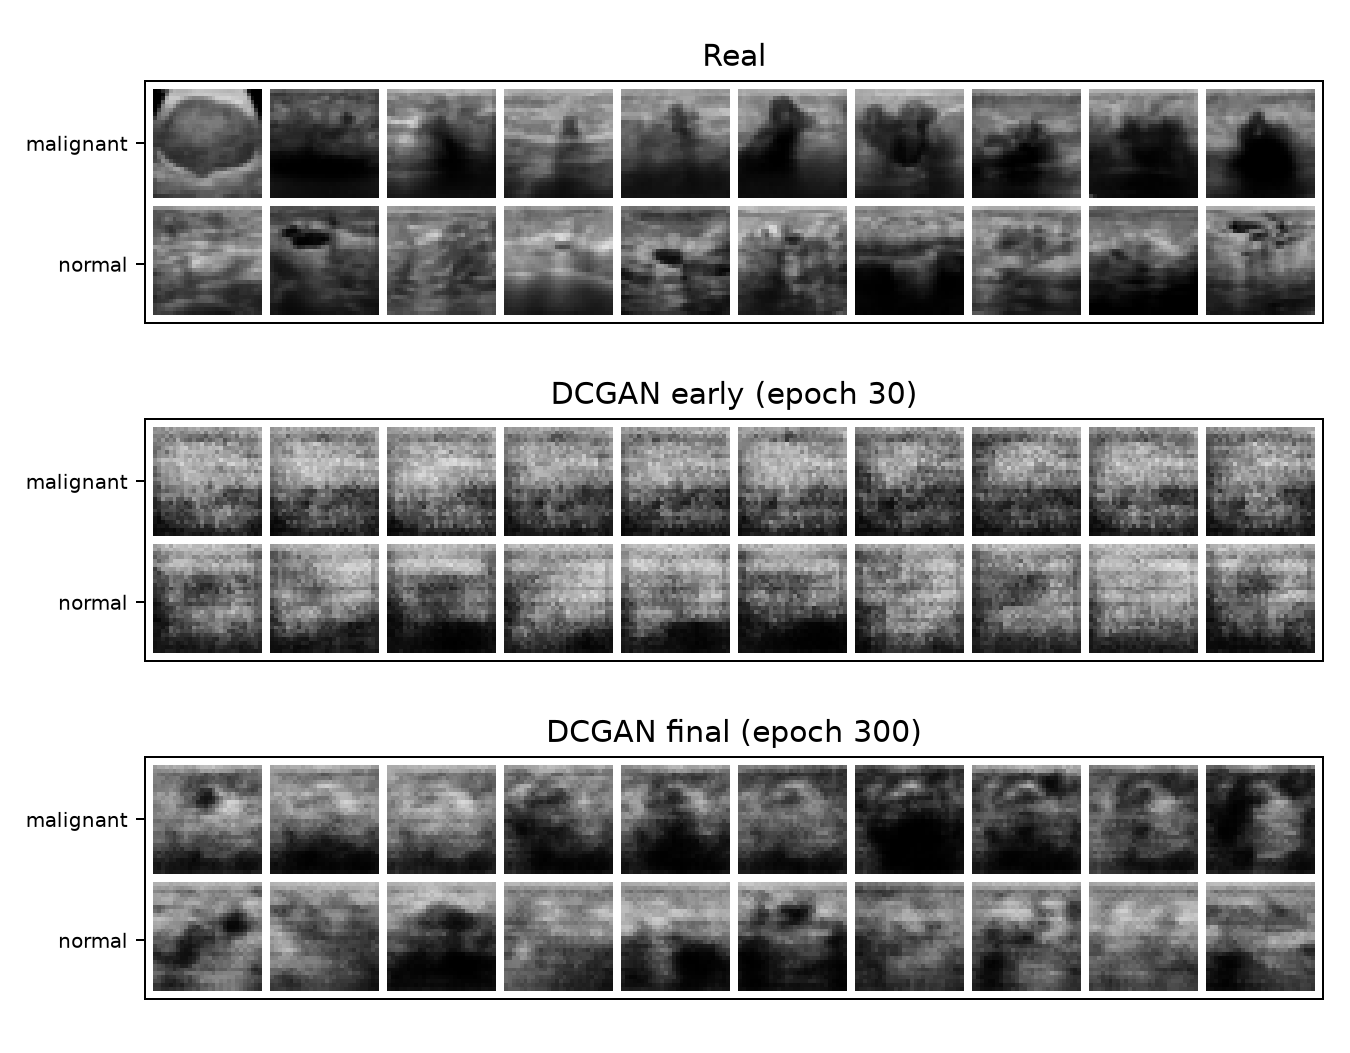
\includegraphics[width=0.9\linewidth]{figures/breast_real_vs_synthetic.png}
\caption{BreastMNIST: real training images (top), early generator after 30 epochs (middle) and final generator after 300
epochs (bottom); one row per class.}
\label{fig:samples}
\end{figure}

\textbf{FID and KID.} Table~\ref{tab:fid} quantifies the quality difference. The final generator reduces FID from 134.9 to
86.4 and KID by about half, but a gap to the real-vs-real reference (59.1) remains: the synthetic distribution is
clearly closer to the real one, yet not identical.

\begin{table}[htbp]
\centering
\caption{Image quality on BreastMNIST (546 images per set; lower is better). Source: \texttt{results/breastmnist/fid.json}.}
\label{tab:fid}
\small
\begin{tabular}{lrr}
\toprule
Compared with real training images & FID & KID \\
\midrule
Real test images (reference floor)   & 59.1  & 0.0004 \\
Early generator (epoch 30)           & 134.9 & 0.1220 \\
Final generator (epoch 300)          & 86.4  & 0.0670 \\
\bottomrule
\end{tabular}
\end{table}

\textbf{No memorisation.} The median distance from a generated image to its nearest training image is 6.33 (final) and
6.96 (early), larger than the 5.52 measured for real test images, and \emph{none} of the generated images is closer to a
training image than the closest 5\% of real test images (fraction 0.00 for both generators). Figure~\ref{fig:nn} shows
generated images next to their nearest training images: they share style but are not copies. The same figure also
shows a weakness: the first two generated images are almost identical to each other, a sign of \emph{limited diversity}
(partial mode collapse) -- the generator does not copy training images, but it also covers fewer distinct variations
than the real data. The latent interpolation in
Figure~\ref{fig:interp} changes smoothly from one image to another, which indicates that the generator learned a continuous
image distribution rather than a lookup table of training images.

\begin{figure}[htbp]
\centering
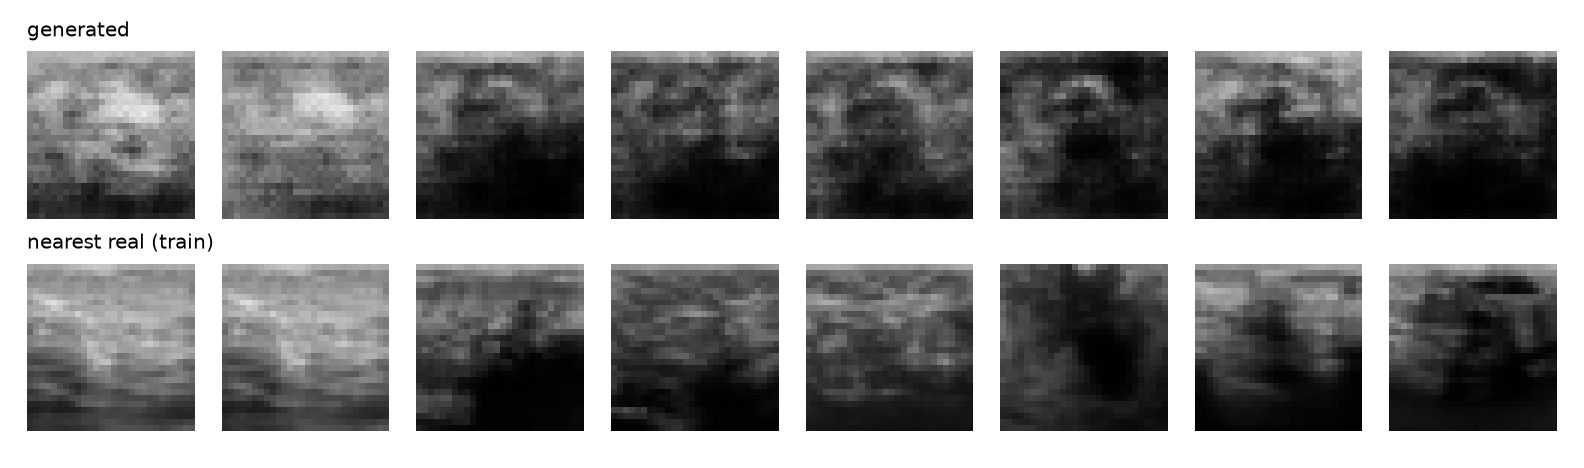
\includegraphics[width=\linewidth]{figures/breast_nearest_neighbours.png}
\caption{Top: images from the final generator. Bottom: the closest real training image to each (pixel $L_2$). Similar
style, different content: the generator does not copy training images. The first two samples are near-duplicates of
each other, showing limited sample diversity.}
\label{fig:nn}
\end{figure}

\begin{figure}[htbp]
\centering
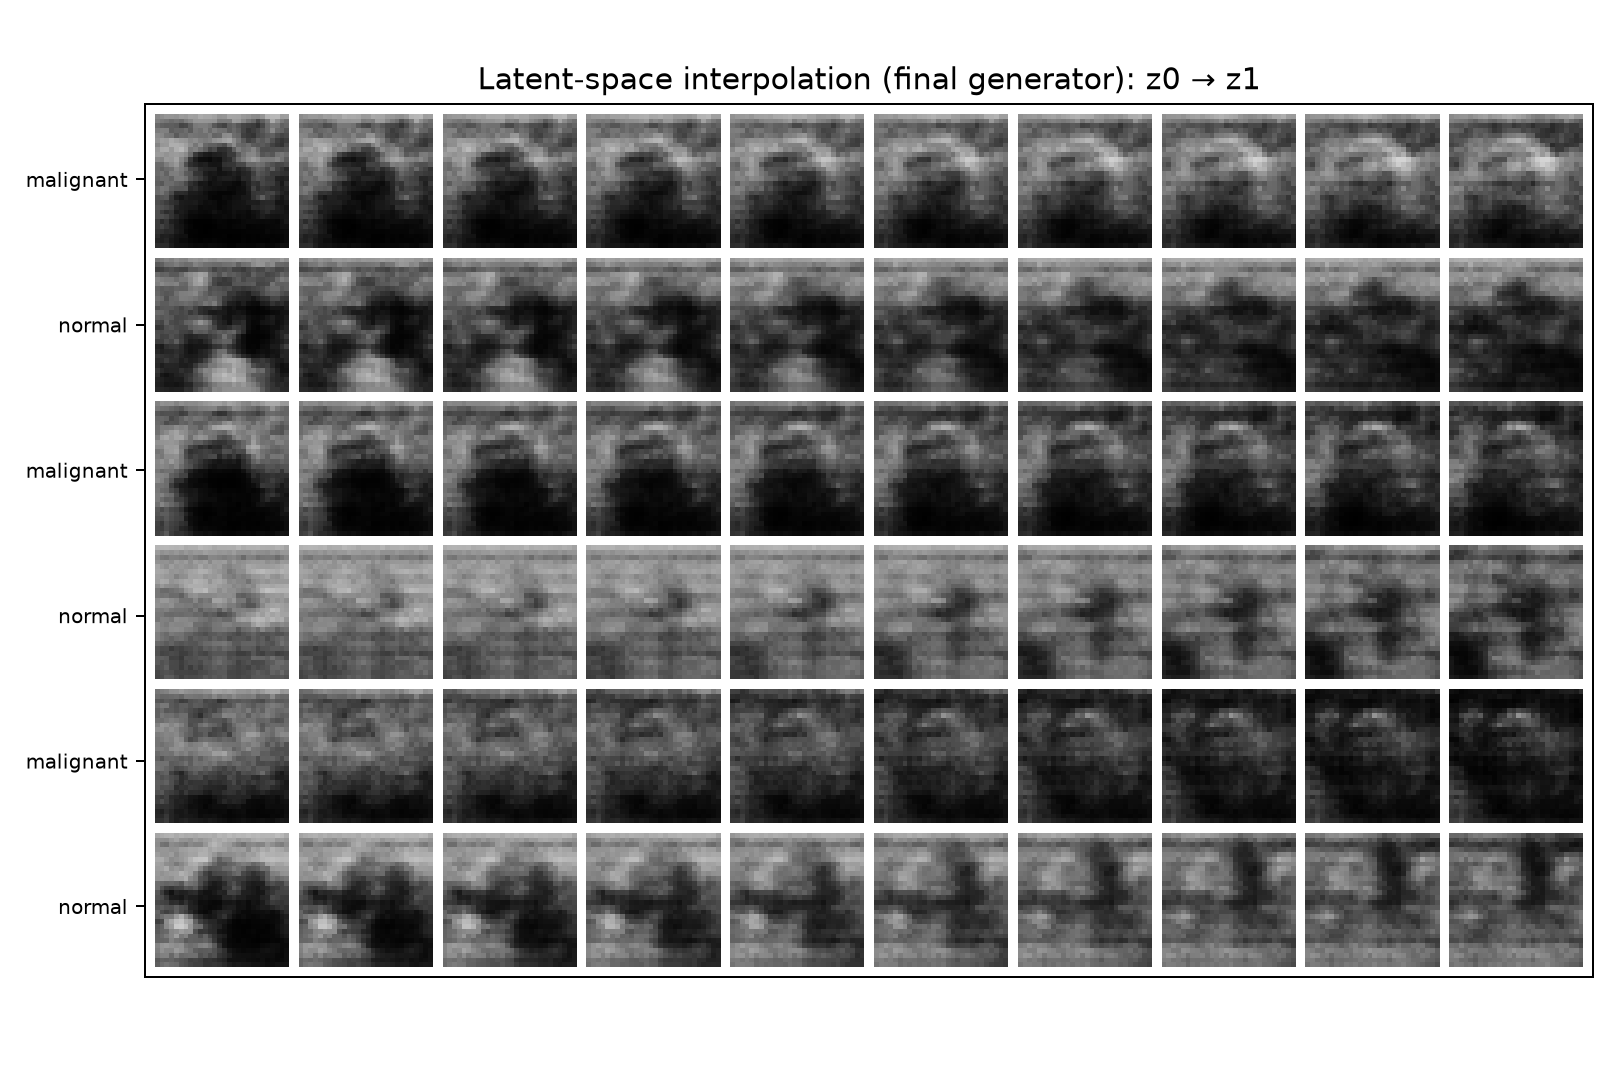
\includegraphics[width=0.85\linewidth]{figures/breast_interpolation.png}
\caption{Linear interpolation between two noise vectors $z_0\to z_1$ (final generator, class fixed per row). Smooth
transitions indicate a continuous learned distribution.}
\label{fig:interp}
\end{figure}

% -------------------------------------------------------------------------------------
\subsection{Does synthetic data help the classifier? (BreastMNIST)}
Table~\ref{tab:breast} and Figure~\ref{fig:ratio} give the main result; Table~\ref{tab:recall} breaks recall down by class.
Our real-only baseline (accuracy 0.856, AUC 0.911) matches the ResNet-18 reference of MedMNIST v2 (0.863 / 0.901), so the
comparison starts from a sound baseline.

\begin{table}[htbp]
\centering
\caption{BreastMNIST, real test set (156 images), mean $\pm$ std over 5 seeds. $\Delta$F1: change in mean macro F1 vs.\
real only; $p$: Welch's $t$-test on per-seed F1 vs.\ real only. Source: \texttt{results/breastmnist/results\_table.md}.}
\label{tab:breast}
\resizebox{\linewidth}{!}{%
\begin{tabular}{lccccccc}
\toprule
Setting & Accuracy & Precision & Recall & Macro F1 & AUC & $\Delta$F1 & $p$ \\
\midrule
Real only (0\%)      & 0.856 $\pm$ 0.013 & 0.829 $\pm$ 0.028 & 0.806 $\pm$ 0.023 & 0.812 $\pm$ 0.012 & 0.911 $\pm$ 0.014 & --     & --    \\
Real + flip/shift    & 0.868 $\pm$ 0.024 & 0.835 $\pm$ 0.031 & 0.837 $\pm$ 0.028 & \textbf{0.834 $\pm$ 0.026} & 0.914 $\pm$ 0.010 & +0.022 & 0.150 \\
\midrule
+50\% GAN (final)    & 0.831 $\pm$ 0.083 & 0.827 $\pm$ 0.059 & 0.794 $\pm$ 0.045 & 0.788 $\pm$ 0.070 & 0.914 $\pm$ 0.016 & $-$0.024 & 0.491 \\
+100\% GAN (final)   & 0.819 $\pm$ 0.046 & 0.816 $\pm$ 0.063 & 0.770 $\pm$ 0.089 & 0.758 $\pm$ 0.080 & 0.908 $\pm$ 0.017 & $-$0.054 & 0.206 \\
+200\% GAN (final)   & 0.858 $\pm$ 0.012 & 0.840 $\pm$ 0.024 & 0.788 $\pm$ 0.040 & 0.805 $\pm$ 0.027 & \textbf{0.922 $\pm$ 0.014} & $-$0.008 & 0.592 \\
\midrule
+50\% GAN (early)    & 0.833 $\pm$ 0.030 & 0.830 $\pm$ 0.046 & 0.758 $\pm$ 0.085 & 0.763 $\pm$ 0.077 & 0.904 $\pm$ 0.012 & $-$0.050 & 0.225 \\
+100\% GAN (early)   & 0.828 $\pm$ 0.042 & 0.792 $\pm$ 0.032 & 0.822 $\pm$ 0.021 & 0.797 $\pm$ 0.036 & 0.898 $\pm$ 0.020 & $-$0.015 & 0.417 \\
+200\% GAN (early)   & 0.847 $\pm$ 0.036 & 0.842 $\pm$ 0.031 & 0.775 $\pm$ 0.097 & 0.780 $\pm$ 0.095 & 0.906 $\pm$ 0.010 & $-$0.032 & 0.490 \\
\midrule
GAN class balancing  & 0.864 $\pm$ 0.019 & 0.838 $\pm$ 0.013 & 0.811 $\pm$ 0.051 & 0.819 $\pm$ 0.039 & 0.916 $\pm$ 0.018 & +0.006 & 0.742 \\
\bottomrule
\end{tabular}}
\end{table}

\begin{figure}[htbp]
\centering
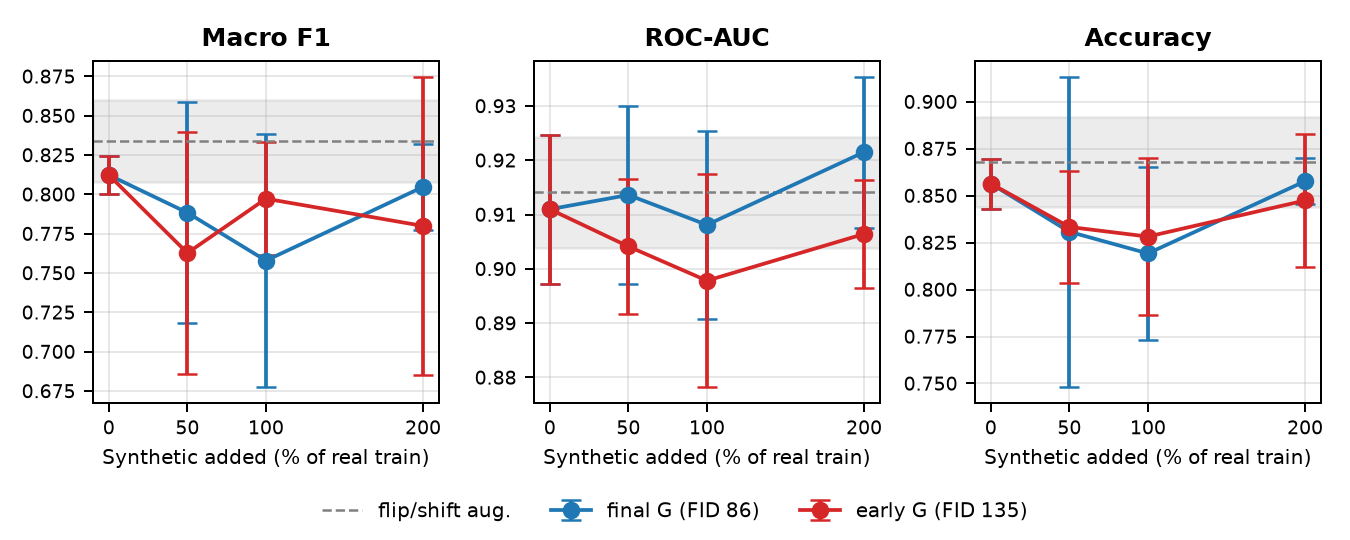
\includegraphics[width=\linewidth]{figures/breast_metrics_vs_ratio.png}
\caption{BreastMNIST: macro F1, ROC-AUC and accuracy against the amount of synthetic data (0\% = real only), for the
final (blue, FID 86) and early (red, FID 135) generator. Error bars: std over 5 seeds. Grey dashed line and band:
classical flip/shift augmentation (mean $\pm$ std).}
\label{fig:ratio}
\end{figure}

\begin{table}[htbp]
\centering
\caption{BreastMNIST per-class recall (mean over 5 seeds; from \texttt{confusion\_matrices.json}). The malignant class is
the clinically important minority class (42 test images).}
\label{tab:recall}
\small
\begin{tabular}{lcc}
\toprule
Setting & Malignant recall & Benign recall \\
\midrule
Real only           & 0.695 $\pm$ 0.085 & 0.916 \\
Real + flip/shift   & \textbf{0.771 $\pm$ 0.069} & 0.904 \\
+50\% GAN (final)   & 0.714 $\pm$ 0.181 & 0.874 \\
+100\% GAN (final)  & 0.662 $\pm$ 0.263 & 0.877 \\
+200\% GAN (final)  & 0.638 $\pm$ 0.106 & 0.939 \\
+100\% GAN (early)  & 0.810 $\pm$ 0.087 & 0.835 \\
GAN class balancing & 0.695 $\pm$ 0.124 & 0.926 \\
\bottomrule
\end{tabular}
\end{table}

\begin{figure}[htbp]
\centering
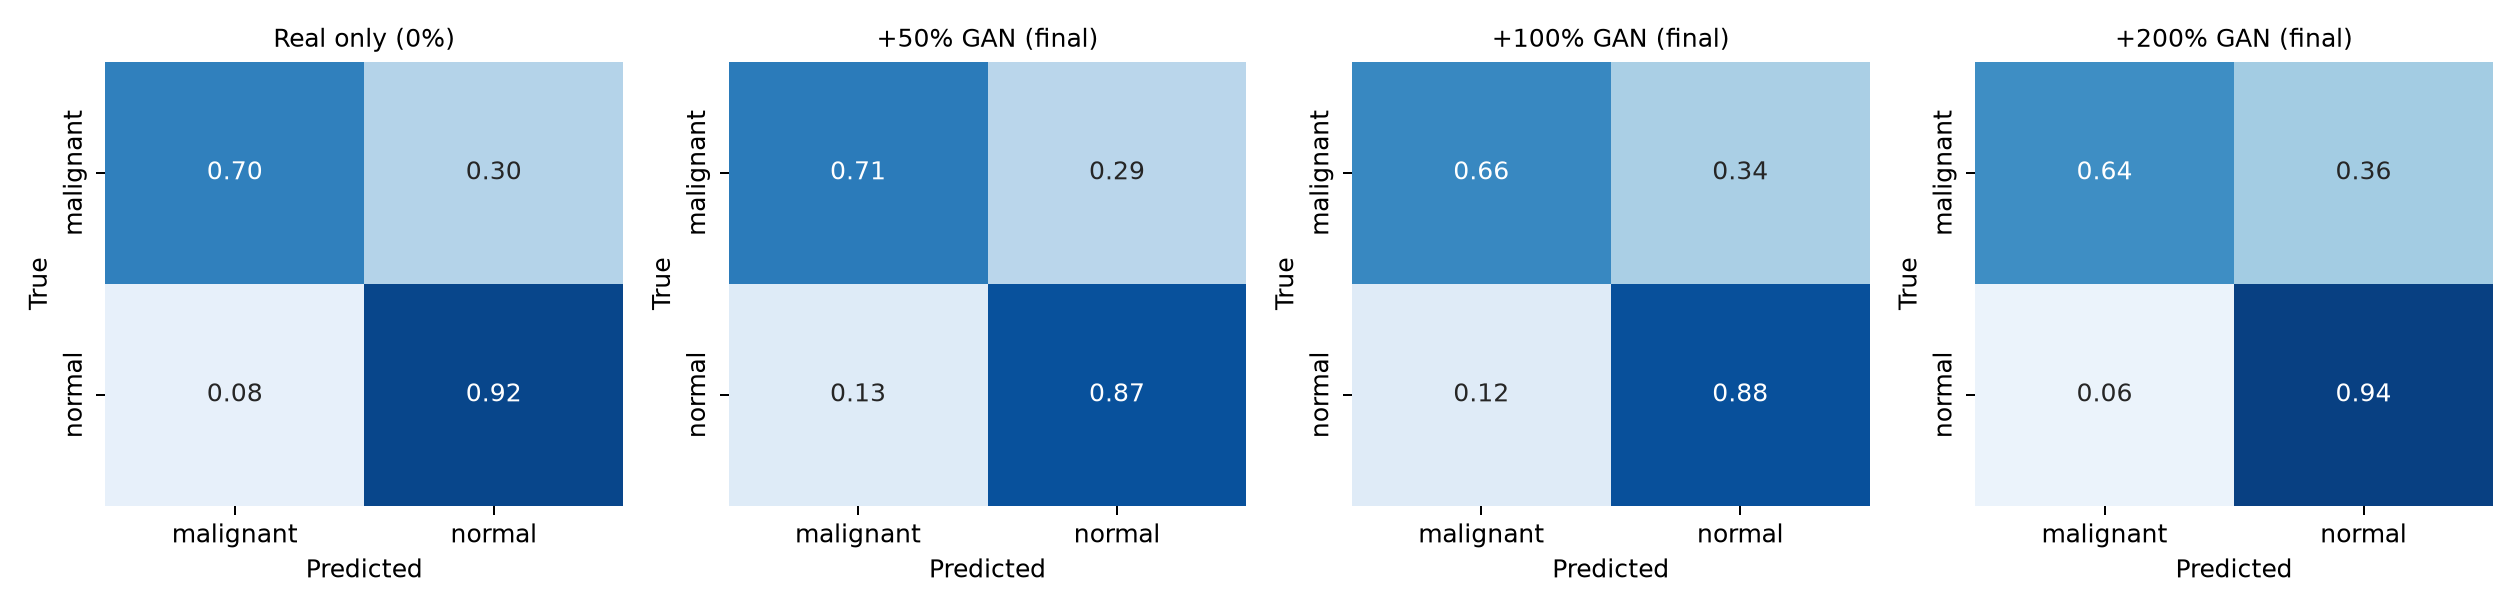
\includegraphics[width=\linewidth]{figures/breast_confusion.png}
\caption{BreastMNIST confusion matrices summed over 5 seeds and normalised per true class (diagonal = per-class recall)
for 0, 50, 100 and 200\% synthetic data from the final generator.}
\label{fig:confusion}
\end{figure}

\noindent The main observations are:
\begin{enumerate}
  \item \textbf{No GAN setting improves macro F1 over real-only training.} Mean F1 changes by between $-0.054$ and
        $+0.006$, and no difference is statistically significant (all $p>0.2$). Accuracy also does not improve
        (best: 0.864 with class balancing vs.\ 0.856).
  \item \textbf{Synthetic data makes training less stable.} The standard deviation of F1 over seeds grows from 0.012
        (real only) to as much as 0.095. With synthetic images in the training set the result depends much more on the
        random seed; e.g.\ one seed of +50\% (final) reached only 0.686 accuracy.
  \item \textbf{Quantity: the effect is not monotonic.} With the final generator, F1 first drops (50\%, 100\%) and then
        recovers almost to the baseline at 200\% (0.805). The +200\% setting gives the \emph{highest AUC} of all
        settings (0.922 vs.\ 0.911), i.e.\ slightly better ranking of cases, but it predicts ``benign'' more often:
        malignant recall falls to 0.638 while benign recall rises to 0.939 (Table~\ref{tab:recall}).
  \item \textbf{Quality matters for AUC.} At every ratio the better generator gives a higher AUC than the early one
        (0.914 vs.\ 0.904, 0.908 vs.\ 0.898, 0.922 vs.\ 0.906). Low-quality images (FID 135) lower AUC below the real-only
        baseline at every ratio. For F1 the picture is mixed and within the seed noise.
  \item \textbf{Classical augmentation is the strongest method.} Random flips and shifts give the best F1 (0.834,
        $+0.022$), the best accuracy (0.868) and raise malignant recall from 0.695 to 0.771 -- at no extra cost and with
        no generator. The difference is not significant at 5 seeds ($p=0.15$), but it is the only consistent positive trend.
  \item \textbf{GAN class balancing is neutral.} Adding 252 synthetic malignant images (to 399 vs.\ 399) leaves F1
        (0.819) and malignant recall (0.695) essentially unchanged: the synthetic minority images did not teach the
        classifier anything about malignant lesions that the 147 real ones did not.
\end{enumerate}

\FloatBarrier
\subsection{Second dataset: PneumoniaMNIST}
PneumoniaMNIST has nine times more real training images (4{,}708). Here the conditional DCGAN produces convincing chest
X-rays (Figure~\ref{fig:pneu_samples}): synthetic \emph{normal} images show clear lung fields and synthetic
\emph{pneumonia} images show hazy, opaque lungs, i.e.\ the class condition is respected. FID against 2{,}000 real training
images is 108.1 for the final and 193.3 for the early generator (real-vs-real reference: 25.3), and only
1.9\% of the generated images are closer to a training image than the closest 5\% of real test images -- fewer than
the 5\% expected for unseen real images, so again there is no memorisation. The quality gap is larger than on
BreastMNIST relative to the reference (108.1 vs.\ 25.3), even though the samples look convincing to the eye.

\begin{figure}[htbp]
\centering
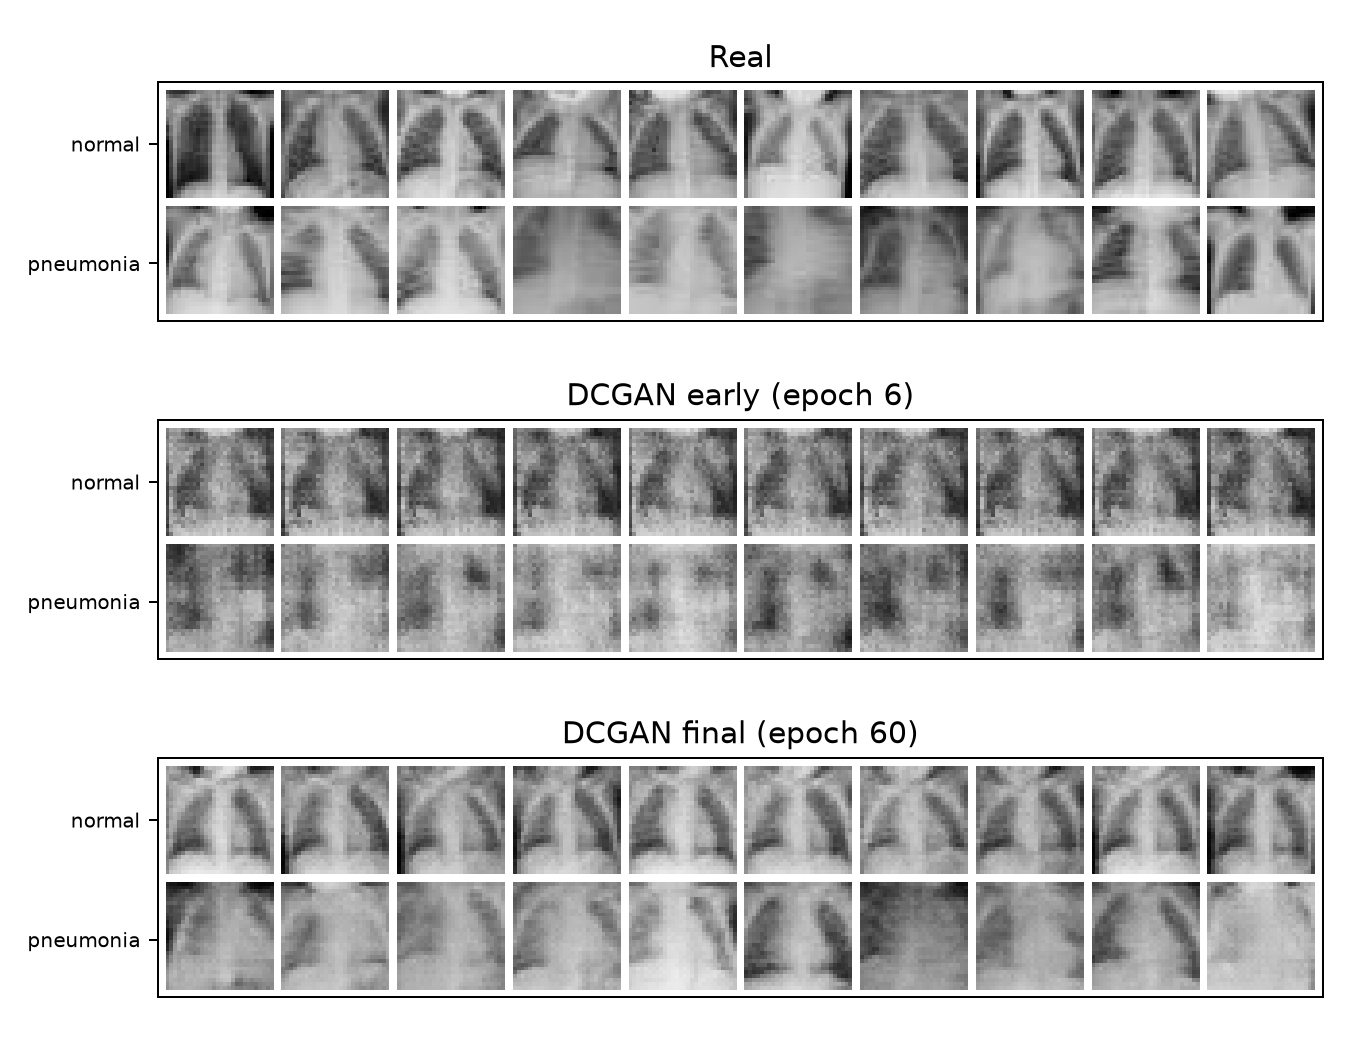
\includegraphics[width=0.9\linewidth]{figures/pneumonia_real_vs_synthetic.png}
\caption{PneumoniaMNIST: real training images (top), early generator after 6 epochs (middle), final generator after 60
epochs (bottom); one row per class.}
\label{fig:pneu_samples}
\end{figure}

\begin{table}[htbp]
\centering
\caption{PneumoniaMNIST, real test set (624 images), mean $\pm$ std over 3 seeds, 15 classifier epochs. $p$: Welch's
$t$-test on per-seed macro F1 vs.\ real only. Normal recall = recall of the minority class \emph{normal}.
Source: \texttt{results/pneumoniamnist/}.}
\label{tab:pneu}
\resizebox{\linewidth}{!}{%
\begin{tabular}{lcccccc}
\toprule
Setting & Accuracy & Macro F1 & AUC & Normal recall & $\Delta$F1 & $p$ \\
\midrule
Real only (0\%)     & \textbf{0.880 $\pm$ 0.017} & \textbf{0.861 $\pm$ 0.021} & 0.973 $\pm$ 0.006 & \textbf{0.691} & --       & --    \\
Real + flip/shift   & 0.808 $\pm$ 0.069 & 0.755 $\pm$ 0.104 & 0.972 $\pm$ 0.010 & 0.489 & $-$0.106 & 0.215 \\
\midrule
+50\% GAN (final)   & 0.860 $\pm$ 0.026 & 0.834 $\pm$ 0.035 & 0.973 $\pm$ 0.005 & 0.634 & $-$0.027 & 0.334 \\
+100\% GAN (final)  & 0.873 $\pm$ 0.006 & 0.853 $\pm$ 0.008 & 0.975 $\pm$ 0.002 & 0.668 & $-$0.008 & 0.573 \\
+200\% GAN (final)  & 0.875 $\pm$ 0.003 & 0.855 $\pm$ 0.004 & \textbf{0.976 $\pm$ 0.002} & 0.671 & $-$0.006 & 0.652 \\
+100\% GAN (early)  & 0.868 $\pm$ 0.005 & 0.845 $\pm$ 0.006 & 0.973 $\pm$ 0.001 & 0.651 & $-$0.016 & 0.317 \\
GAN class balancing & 0.863 $\pm$ 0.015 & 0.838 $\pm$ 0.019 & 0.973 $\pm$ 0.002 & 0.635 & $-$0.023 & 0.240 \\
\bottomrule
\end{tabular}}
\end{table}

\begin{figure}[htbp]
\centering
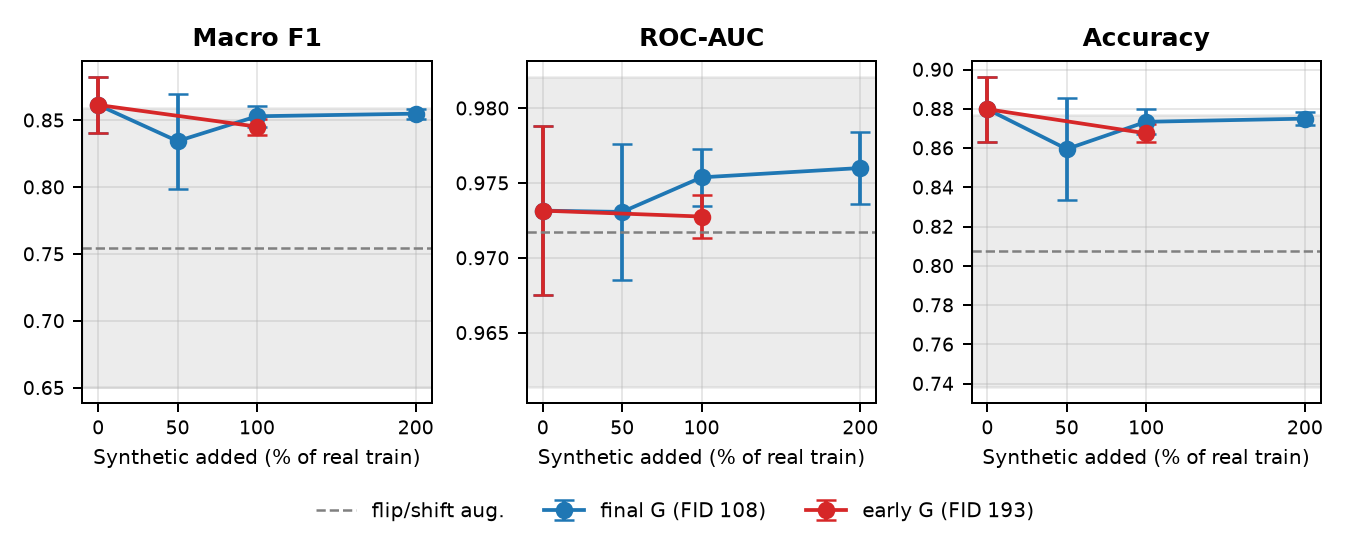
\includegraphics[width=\linewidth]{figures/pneumonia_metrics_vs_ratio.png}
\caption{PneumoniaMNIST: metrics against the amount of synthetic data. Note how the error bars shrink as more synthetic
images are added, while the means stay at the real-only level.}
\label{fig:pneu_ratio}
\end{figure}

\noindent Table~\ref{tab:pneu} and Figure~\ref{fig:pneu_ratio} show the same overall answer as on BreastMNIST, with two
instructive differences:
\begin{enumerate}
  \item \textbf{Again, no F1 gain.} No GAN setting beats the real-only baseline (F1 0.861); differences range from
        $-0.027$ to $-0.006$ and none is significant (all $p>0.2$). The real-only baseline (accuracy 0.880, AUC 0.973)
        is above the MedMNIST v2 ResNet-18 reference (0.854 / 0.944).
  \item \textbf{Synthetic data stabilises training here.} The seed-to-seed standard deviation of F1 falls from 0.021
        (real only) to 0.008 (+100\%) and 0.004 (+200\%), and the +200\% setting has the highest AUC (0.976). With a
        larger real set, the GAN is a better model of the data and its images act as a mild regulariser.
  \item \textbf{Quality still matters.} At +100\%, the final generator beats the early one on every metric (F1 0.853
        vs.\ 0.845, AUC 0.975 vs.\ 0.973, normal recall 0.668 vs.\ 0.651).
  \item \textbf{Classical augmentation hurts on chest X-rays.} Horizontal flipping drops F1 to 0.755 and normal recall to
        0.489. A mirrored chest X-ray puts the heart on the wrong side -- an anatomically impossible image -- whereas a
        mirrored breast ultrasound is still realistic. Augmentation must respect the anatomy of the modality.
  \item \textbf{All models under-detect the normal class.} Pneumonia recall is above 0.99 in every setting, but normal
        recall is only 0.49--0.69, so most errors are normal patients predicted as pneumonia. Neither proportional
        augmentation nor GAN class balancing (normal recall 0.635) fixed this.
\end{enumerate}

% -------------------------------------------------------------------------------------
\FloatBarrier
\section{Discussion}
\textbf{Answer to the research question.} In our setting, adding DCGAN-generated images did \emph{not} improve a CNN
classifier on real test images, on either dataset, at any amount (50--200\%) or quality (FID 86 vs.\ 135). This
differs from the improvement reported by Frid-Adar et al.~\cite{fridadar2018gan}, and we see four reasons in our results.

\begin{enumerate}
  \item \textbf{A GAN cannot add information it never saw.} The generator is trained on the same 546 (or 4{,}708)
        images as the classifier. Our memorisation check shows that it does not copy them, but the samples are
        variations of the same visual content -- with limited diversity (near-duplicate samples, Figure~\ref{fig:nn}).
        New \emph{information} about rare cases (e.g.\ unusual malignant lesions) can only come from new real data.
  \item \textbf{The quality gap acts like label noise.} With FID 86 against a real-vs-real floor of 59, part of the
        synthetic images are not clearly typical of their class. When such images make up a third to two thirds of the
        training set, the classifier partly learns GAN artefacts and ambiguous class boundaries; on BreastMNIST this
        shows up as a lower and less stable F1 at 50--100\%.
  \item \textbf{Quantity helps ranking more than decisions.} At 200\%, AUC is the best of all settings on both datasets
        (0.922 and 0.976), so synthetic images seem to regularise the learned features; but the decision threshold
        shifts towards the majority class (malignant recall 0.638). A threshold tuned on validation data might
        turn this AUC gain into an F1 gain -- a cheap follow-up experiment.
  \item \textbf{Better images help, but not enough.} The final generator beats the early one in AUC at every BreastMNIST
        ratio and on every PneumoniaMNIST metric, so quality clearly matters; the trend suggests that a stronger
        generator (StyleGAN2-ADA, diffusion) is a prerequisite for gains, not an option.
\end{enumerate}

\textbf{Dataset size changes the role of synthetic data.} With 546 images, synthetic data mainly added variance; with
4{,}708 images it reduced variance (std of F1 from 0.021 to 0.004). A GAN trained on more data is a better model of
that data, and its samples then behave like a smooth regulariser rather than noise.

\textbf{Classical augmentation must match the modality.} Simple flips and shifts were the best method for breast
ultrasound (F1 +0.022, malignant recall +0.076) but the worst for chest X-rays (F1 $-0.106$), because a mirrored chest is
anatomically wrong. Domain knowledge matters more than the sophistication of the augmentation method.

\textbf{Why multiple seeds were essential.} With a single seed we could have reported almost any conclusion: individual
BreastMNIST runs of +50\% GAN range from accuracy 0.686 to 0.891. Only the mean over seeds, the standard deviation and the
$t$-test reveal that none of the differences is reliable -- a methodological point that much of the GAN-augmentation
literature does not address.

\textbf{Practical recommendation.} For a small medical dataset, first use modality-appropriate classical augmentation and
report results over several seeds; consider GAN augmentation only with a generator whose FID is close to the real-vs-real
floor, check it for memorisation, and evaluate it against the classical baseline as done here.

\section{Limitations and Future Work}
\begin{itemize}
  \item \textbf{Resolution.} We used 28$\times$28 images to fit a CPU budget; fine lesion details are lost. MedMNIST+ offers
        64--224\,px versions on which both the GAN and the classifier could behave differently.
  \item \textbf{Generator family.} DCGAN is a 2016 architecture. StyleGAN2-ADA or diffusion models produce markedly better
        samples on small datasets and may change the conclusion.
  \item \textbf{Metric mismatch.} FID relies on ImageNet features that are poorly suited to grayscale ultrasound; a
        medical-domain feature extractor would give a more meaningful quality score.
  \item \textbf{Statistics.} Five (three) seeds give a rough estimate of variance; the BreastMNIST test set has only
        42 malignant images, so a single changed prediction moves recall by 2.4 points.
  \item \textbf{Single classifier.} We used one small CNN; a larger or pretrained model may benefit differently from
        synthetic data.
  \item \textbf{No clinical validation.} Synthetic images were not reviewed by radiologists; the system is a research
        prototype, not a diagnostic tool.
\end{itemize}

\section{Conclusion}
We built a complete, reproducible pipeline to test whether GAN-generated images help a classifier trained on a small
medical dataset. A class-conditional DCGAN with DiffAugment-style translation learned realistic-looking breast ultrasound
and chest X-ray images without memorising its training data, and a better generator (lower FID) consistently gave better
classifiers than a worse one. Nevertheless, adding 50--200\% synthetic images did not improve macro F1 on real test
images for either dataset, and no difference was statistically significant over 5 (3) seeds. Synthetic data raised AUC
slightly at 200\% and, on the larger dataset, made training much more stable, while simple flip/shift augmentation was the
best method for ultrasound but harmful for chest X-rays. The answer to ``does synthetic data help?'' is therefore:
\emph{not by itself with a DCGAN at this scale -- quality, dataset size and the choice of baseline decide}.
Future work: higher resolution (MedMNIST+), stronger generators (StyleGAN2-ADA, diffusion), threshold tuning, and
filtering synthetic images by classifier confidence before adding them.

\section*{Code Availability and Demo}
Code, results and instructions: \url{https://github.com/Bhagwati23/GAN-medicalAugmentation}. The package \texttt{ganaug}
contains one module per stage (data, DCGAN, GAN training, augmentation, classifier, FID, experiments, report figures);
\texttt{tests/} checks shapes, determinism and that synthetic images never reach the validation or test sets; a GitHub
Actions workflow runs these tests on every pull request. \texttt{app.py} is a Gradio web app that generates synthetic images
for a chosen class and generator checkpoint, classifies an uploaded or real test image with both the real-only and the
GAN-augmented classifier side by side, and shows the result tables.

\section*{Individual Contributions}
\begin{itemize}
  \item \textbf{Arjun Kadam} (su-24022@sitare.org): synthetic-data augmentation pipeline (issue \#5), integration, testing,
        CI and reproducibility (\#8), demo application, project report (\#9).
  \item \textbf{Bhagwati} (su-24032@sitare.org): conditional DCGAN architecture (\#3), GAN training, checkpoints and samples (\#4), independent re-run of GAN training (reproducibility check);
        repository set-up, issue planning, team workflow, and PR review and merge coordination.
  \item \textbf{Maneesh Sakhwar} (su-24068@sitare.org): dataset selection, loading, exploration notebook and data-leakage tests (\#1); FID/KID evaluation
        and memorisation check (\#6).
  \item \textbf{Anand Singh} (su-24014@sitare.org): CNN baseline (\#2); experiment runs, comparison tables and figures (\#7).
\end{itemize}

